\documentclass[11pt,a4paper]{article}
\usepackage[a4paper, total={6in, 9in}]{geometry}
\usepackage[utf8]{inputenc}
\usepackage[german]{babel}
\usepackage[T1]{fontenc}
\usepackage{amsmath}
\usepackage{amsfonts}
\usepackage{amssymb}
\usepackage{graphicx}
\usepackage{listings}
\usepackage{color}
\usepackage{float}  % for 'H' in picture placement
\usepackage{tabularx} % for automatic linebreak in tables
\usepackage[backend=biber,
style=authoryear, % Zitierstil 
natbib=true, 
hyperref=true, % hyperref-Paket für Links
maxbibnames=9, 
firstinits=true,
]{biblatex}

\usepackage{helvet}
\renewcommand{\familydefault}{\sfdefault}

% DEFINES
\newcommand{\guiplotsize}{0.75}
\newcommand{\resultplotsize}{0.9}
\newcommand{\guiversion}{1.0}
\newcommand{\literatureListPadding}{0.1cm}

\addbibresource{literature.bib}


\title{Seminararbeit}
\usepackage[onehalfspacing]{setspace}
\author{Manuel Theurl}
%\usepackage{scrpage2}
\usepackage{scrpage2}

\pagestyle{scrheadings}
\clearscrheadfoot
\setlength{\parindent}{0em} 
%\setfootsepline{0.2pt}

\begin{document}


%\ifoot{{\small Manuel Theurl}}
%\cfoot{{\small \today}}
%\ofoot{{\small \pagemark}}

%Titelseite:
\begin{titlepage}

\vspace{5cm}



\includegraphics[width=0.18\textwidth]{pictures/logo_uni_graz.jpg}
\hfill

\includegraphics[width=0.18\textwidth]{pictures/logo_geo_raum.jpg}



\begin{center}

\vspace{1.5cm}

\textbf{\Large Energiebilanz im Ablationsgebiet der Pasterze}\\
\vspace{2cm}
\textsc{\Large {Bachelorarbeit}}\\
\vspace{1.5cm}
zur Erlangung des akademischen Grades\\
\vspace{1cm}
\textbf{Bachelor of Science}\\
\vspace{1cm}
der Studienrichtung Umweltsystemwissenschaften - Geographie\\
an der Karl-Franzens-Universität Graz\\
\vspace{1cm}
vorgelegt von\\
\vspace{1cm}
\textbf{Manuel Theurl}\\
\vspace{1cm}
am Institut für: Geographie und Raumforschung\\
\vspace{1cm}
Begutachter: Jakob Abermann, Ass.-Prof. Dr.rer.nat.\\
\vspace{1cm}
Graz, 2019

\end{center}


\end{titlepage} 

\pagebreak
%Inhaltsverzeichnis:
\ofoot{{\small \pagemark}}
\pagenumbering{Roman} 
\section*{Abstract (English)}
The aim of this thesis is to create a model for the energy balance in the ablation area of a glacier by using weather data. The observed glacier in this study is the Pasterze in Austria. The developed program should be a useful tool to edit the data, calculate the energy balance and create visualizations to represent the generated data. Because there are also ablation measurements included in case of the Pasterze, it is possible to compare the measured and modeled melting water..

By comparing the measured and modeled melting water, the validity of the modeled energy balance can be checked. The research question therefore would be, if the model properly represents the reality. With a functioning model the effect of phenomena like ``global dimming’’ and ``global brightening’’ on the melting of the glacier in the ablation area can be examined.\\

All the necessary logic, the calculations and visualizations are done with the programming language Python. The formulas used are mainly taken from \citeauthor{ThePhysicsOfGlaciers} (\citeyear[153-157]{ThePhysicsOfGlaciers}). While programming, a graphical user interface (GUI) will be developed as well. With the GUI the functionality of the software is easy accessible and applicable. The GUI is public, a download and installation description is included in the thesis.\\

As a result the meltwater calculated out of the ablation measurements is strongly correlating with  the modeled meltwater. The model therefore is representing the reality well. Further, it turns out that phenomena like ``global dimming’’ and ``global brightening’’ have a significant impact on the melting of a glacier in the ablation area.
 
\pagebreak
\section*{Abstract}

Ziel dieser Arbeit ist es, aus Wetterdaten ein Modell für die Energiebilanz im Ablationsgebiet eines Gletschers zu finden. Als Beispielgletscher dient hier die Pasterze in Österreich. Es soll ein gesamtheitliches Programm entwickelt werden, das die Aufbereitung der Daten, die Berechnung der Energiebilanz und anschauliche Darstellungsmethoden bietet. Im Falle der Pasterze liegen auch Ablationsmessungen vor, wodurch eine Untersuchung des berechneten sowie des aus der Energiebilanz modellierten Schmelzwassers möglich ist.\\

Es soll somit erörtert werden, ob das Modellieren der Energiebilanz aus Wetterdaten sinnvoll ist und ähnliche Werte für die Ablation bzw. das Schmelzwasser folgen, wie aus den Messungen dazu. Als Forschungsfrage ergbit sich somit, ob das Modell ausreichend der Realität entspricht. Mit dem fertigen Modell kann auch der Fragestellung nachgegangen werden, inwieweit sich die Phänomene ``global dimming'' bzw. ``global brightening'' auf das Abschmelzen des Gletschers im Ablationsgebiet auswirken.\\

Die Untersuchungen erfolgen in der Programmiersprache Python, wobei die Formeln zur Berechnung der Energiebilanz stark an \citeauthor{ThePhysicsOfGlaciers} (\citeyear[153-157]{ThePhysicsOfGlaciers}) angelehnt sind. Im Zuge der Programmierung wird ein GUI mitentwickelt, welches die Funktionalität der Software anschaulich aufbereitet darstellt. Das GUI ist öffentlich zugänglich, eine Beschreibung zum Download und zur Installation ist in der Arbeit ersichtlich.\\

Als Resultat folgt, dass es eine starke Korrelation zwischen dem aus den Ablationsmessungen errechneten Schmelzwasser und dem modellierten Schmelzwasser gibt. Das Modell repräsentiert die Realität somit gut. Weiters stellt sich heraus, dass sich Phänomene wie ``global dimming'' bzw. ``global brightening'' signifikant auf das Abschmelzen eines Gletschers im Ablationsgebiet auswirken.\\


\pagebreak
\section*{Vorwort und Danksagung}
Mein persönlicher Wunsch war es, ein Thema für die Bachelorarbeit zu finden, welches einerseits eine Verbindung zu den Bergen hat und andererseits auch eine herausforderung in Bezug auf Programmierkenntnisse beinhaltet. Als begnadeter Osttiroler Bergläufer und ``Schitouren-Geher'' war die Energiebilanz im Ablationsgebiet der Pasterze somit ein perfektes Thema.\\

Ich danke an dieser Stelle meinem Betreuer Herrn Ass.-Prof. Dr. Abermann Jakob der mir einerseits viel Freiraum zur selbstständigen Gestaltung der Arbeit gelassen hat und mich andererseits tatkräftig mit tollen Ideen, zahlreicher wissenschaftlicher Literatur und nicht zuletzt persönlich bei zahlreichen Treffen unterstützt hat. Ein Dank geht außerdem auch an die Wetterstation bei der Pasterze (TODO Name?), die mir Wetterdaten vom Ablationsgebiet der Pasterze zur Verfügung gestellt hat.\\

Ein Dank geht weiters auch an Roberta Theurl und Luca Braun für das Korrekturlesen der Arbeit. 


\pagebreak

\tableofcontents
\vspace{1cm}

\pagebreak
\listoffigures
\vspace{1cm}

\pagebreak
\listoftables
\vspace{1cm}


\pagebreak
\pagenumbering{arabic}  
\setcounter{page}{1}

\section{Einleitung}
Die Pasterze am Fuße des Großglockners in Österreich (Grenze Osttirol/Kärnten) ist Gegenstand vieler wissenschaftlicher Untersuchungen. Durch eine Betrachtung der Energiebilanz im Ablationsgebiet dieser soll es ermöglicht werden, das Wissen über die Pasterze und vor allem auch über das Abschmelzen dieser zu vertiefen. Anhand von Wetterdaten der Wetterstation bei der Pasterze und geeigneten Energiebilanz-Kalkulationen soll ein Modell generiert werden, welches die Vergangenheit beschreibt, die Gegenwart bestätigt und Prognosen für die Zukunft erstellt. Da auch Ablationsmessungen vorliegen, kann das errechnete und modellierte Schmelzwasser verglichen werden und es können somit auch Aussagen über die Veränderung des Eisdickenverlustes bei Phänomenen wie ``global dimming'' und ``global brightening'' getroffen werden. \\
Die erstellte grafische Benutzeroberfläche bietet die Möglichkeit selber am Thema weiterzuarbeiten, Analysen durchzuführen und bei längeren Zeitreihen Trends zu erkennen. Sofern die benötigten Messdaten vorhanden sind, kann diese grafische Benutzeroberfläche bei jedem beliebigen Gletscher zum Einsatz kommmen.


\section{Theoretisches Grundwissen}
Um die vorgestellte Forschungsfrage und die damit zusammenhängenden Methoden einwandfrei verstehen zu können, braucht es ein gewisses Grundwissen über die Pasterze an sich, über die Energiebilanz sowie über das Phänomen ``global dimming'' bzw. ``Global brigthening''.

\subsection{Pasterze und Ablationsgebiet}
Die Pasterze beim Großglockner ($3798~m$) ist trotz der Abschmelztendenzen nach wie vor der größte Gletscher der Ostalpen. Messungen aus dem Jahre 2006 ergeben eine damalige Länge von $8.3~km$, eine Fläche von $17.3~km^2$ und ein Volumen von $1.7~km^3$ (vgl. \cite[10]{Pasterze}). Der Großglockner und die Pasterze stellen eine ``fachlich perfekte'' Modellregion dar und sind damit wohl stark für die ``österreichische Bergästhetik'' verantwortlich (vgl. \cite[13]{Pasterze}).\\
Die Pasterze hatte um das Jahr 1850 ihren Höchststand. Seit diesem Zeitpunkt nimmt die Eismasse sowie die Gletscherlänge, wie in Abbildung \ref{fig:Längenverluste der Pasterze} ersichtlich, aufgrund klimatischer Veränderungen stetig ab (vgl. \cite[17]{Pasterze}).\\

Die kleine Eiszeit von ca. 1260-1860 zerstörte (durch den Hochstand 1850) Spuren von früheren Vorstößen wie zum Beispiel Moränen. Funde von Holz und Torf vor dem aktuellen Eisrand ergaben jedoch ein Alter von 9000 Jahren, was bedeutet, dass die Pasterze schon zumindest seit dem frühen Holozän existiert (vgl. \cite[24]{Pasterze}).

Folgende Abbildung zeigt einen Überblick vom Großglockner, den umliegenden Bergen und der Pasterze. 
\begin{figure}[H]
\centering
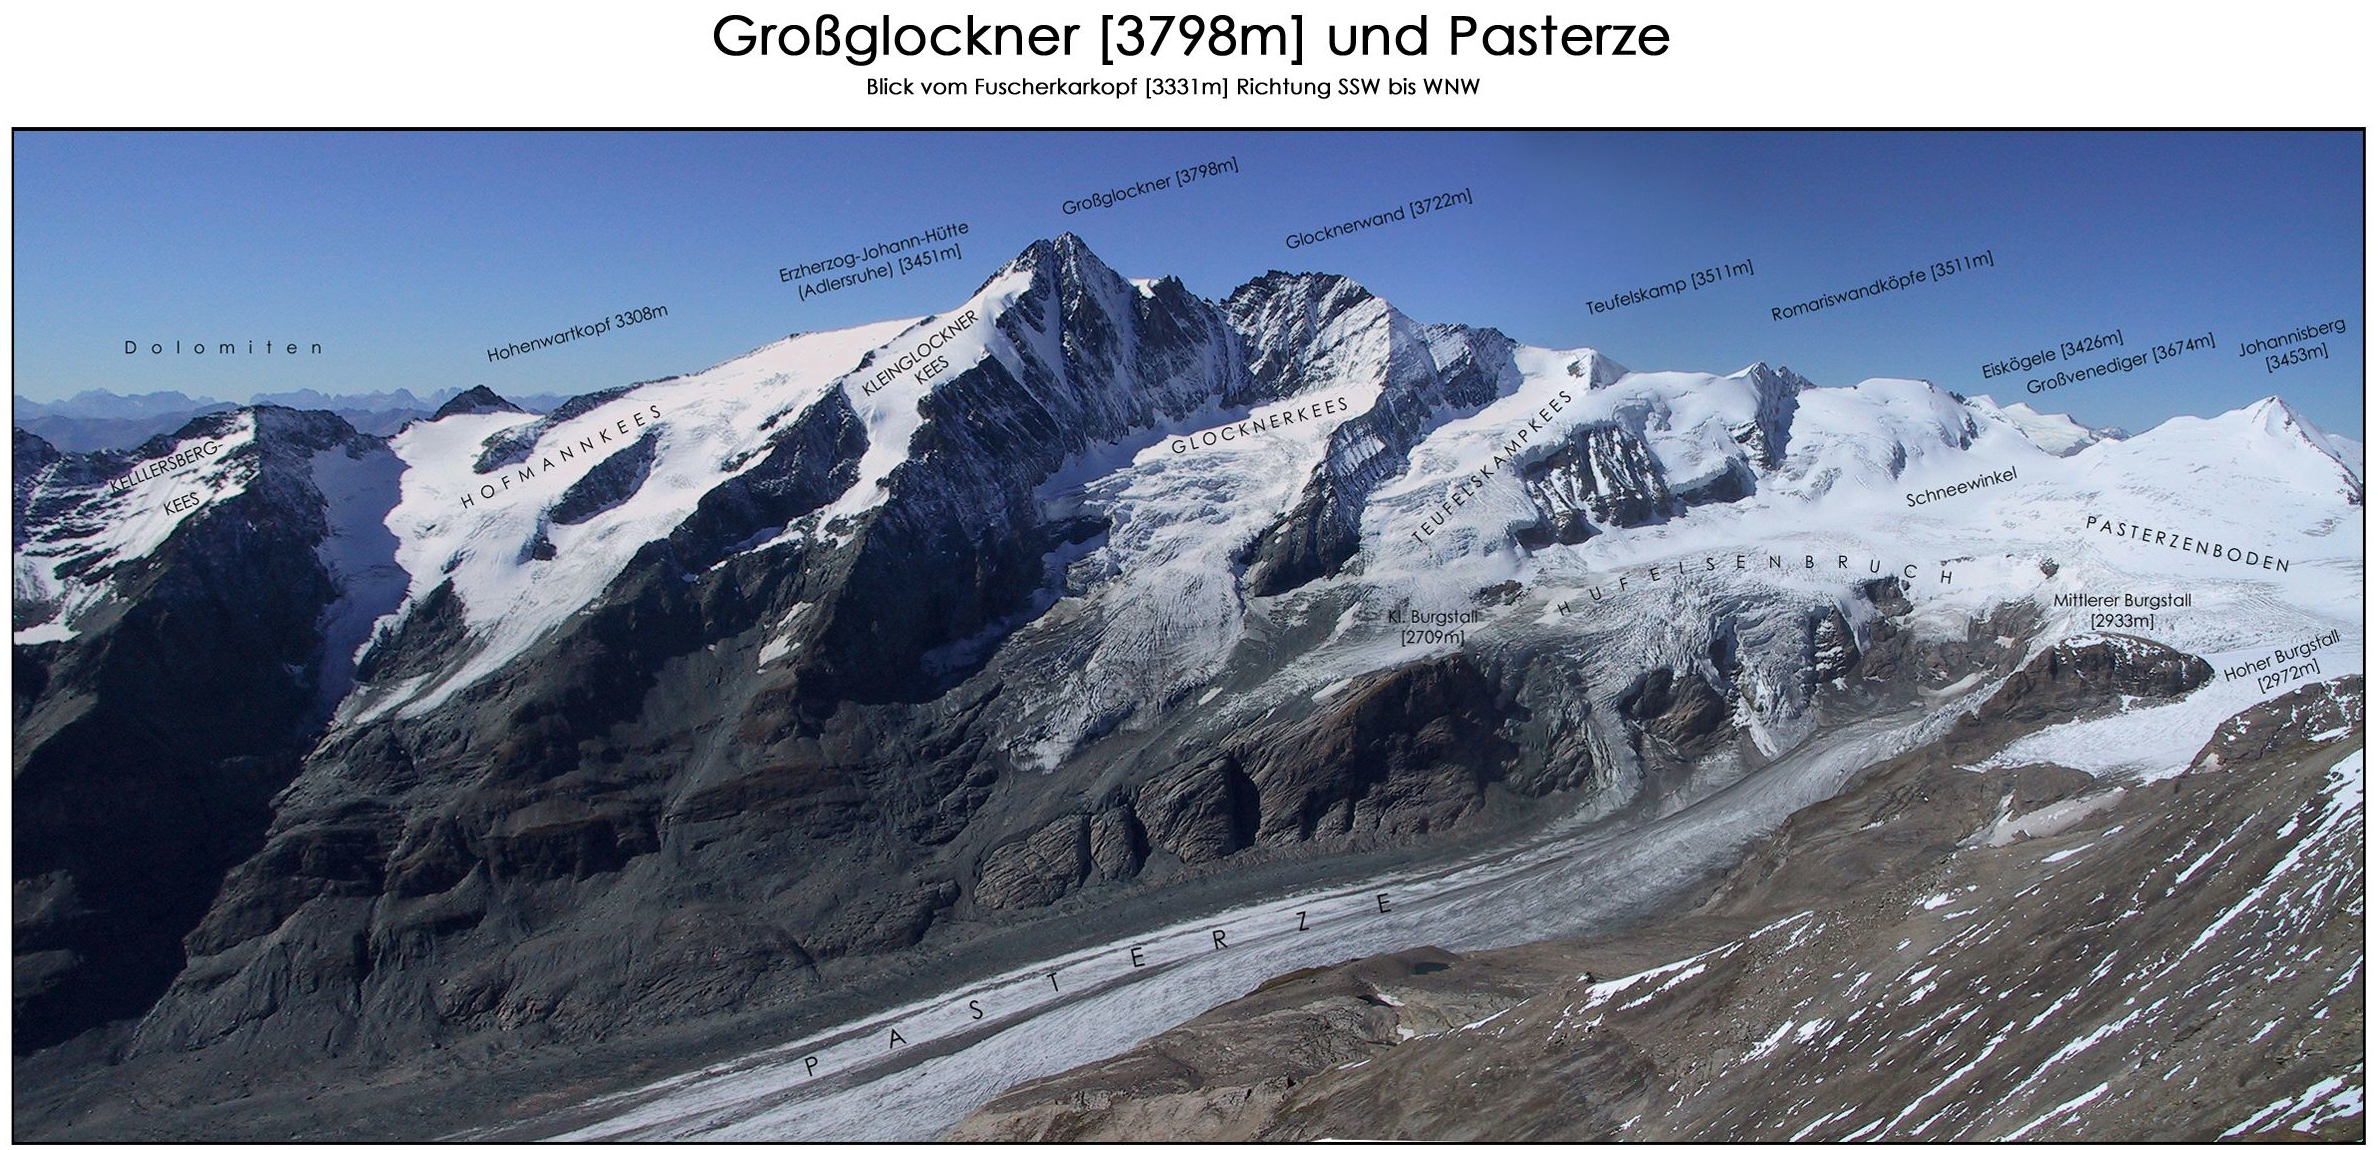
\includegraphics[width=0.9\textwidth]{pictures/Pasterze_Beschriftung_bw.jpg}
\caption[Großglockner und Pasterze]{Großglockner und Pasterze (Foto: Gerhard K. Lieb vom 22.09.2006, Bildbearbeitung: Ulf Oberth)}
\label{fig:Grossglockner und Pasterze}
\end{figure}


Der erwähnte Längenverlust wird mit folgender Abbildung ersichtlich.

% cited correctly??
\begin{figure}[H]
\centering
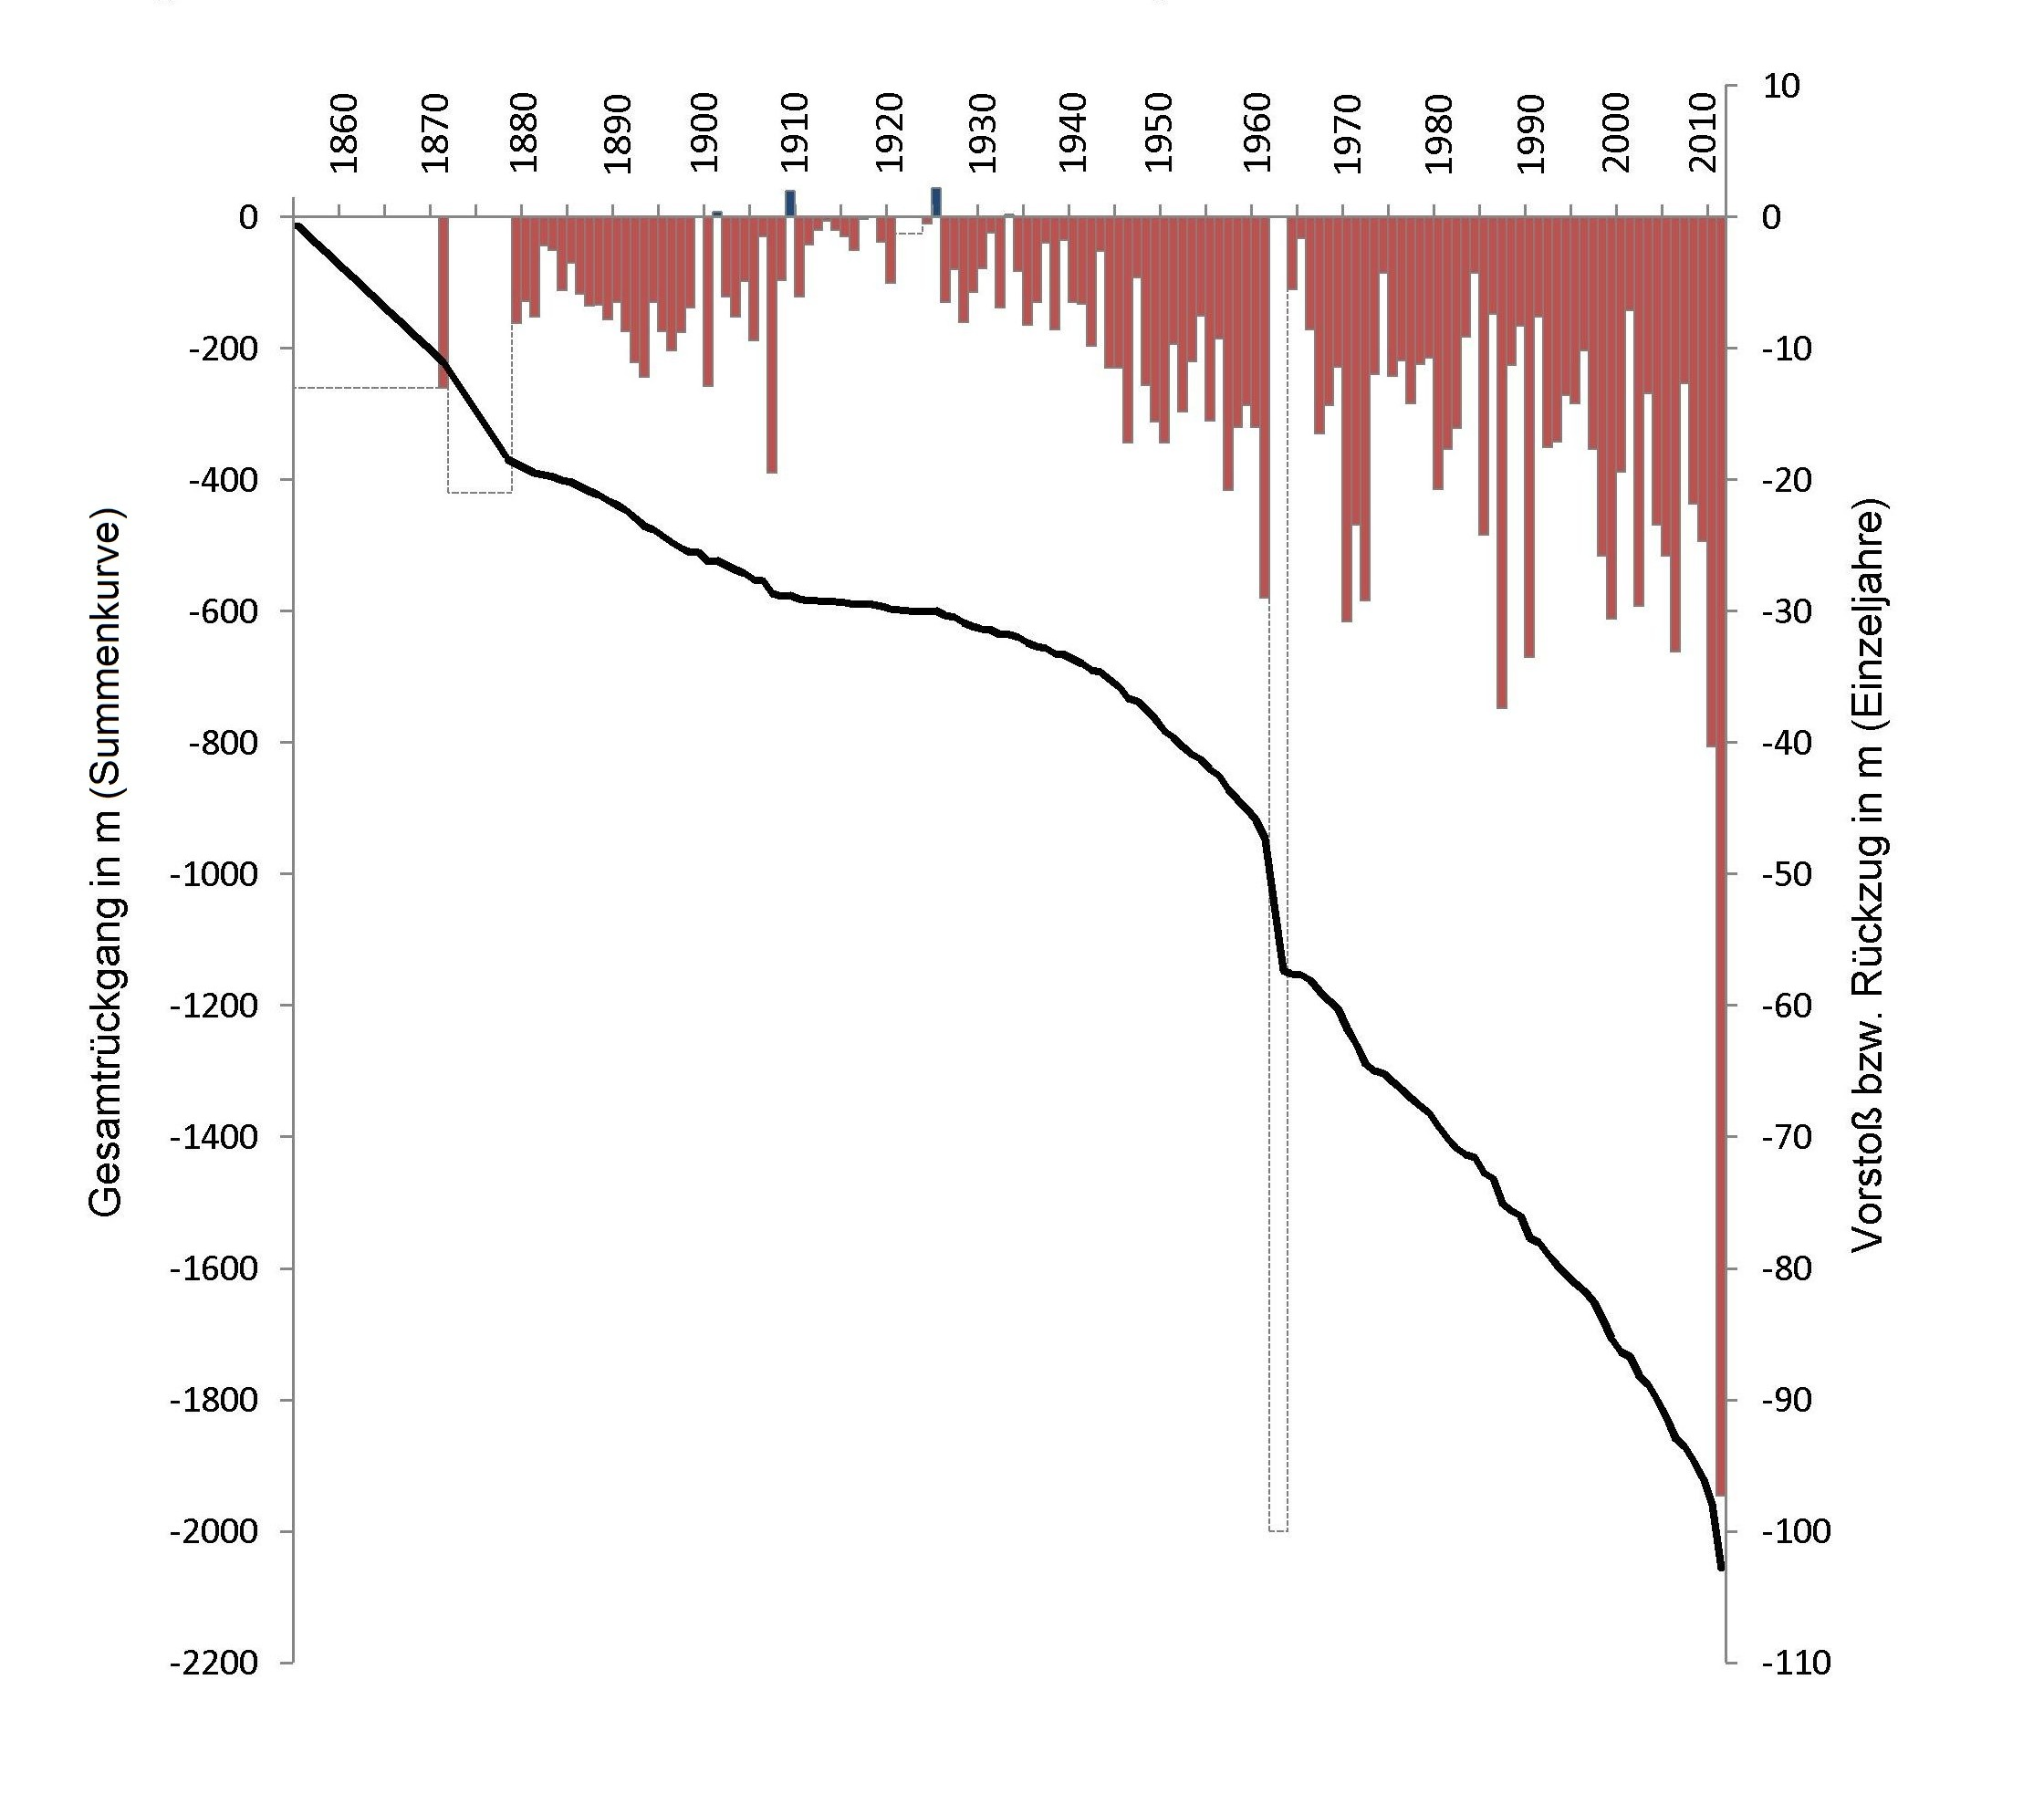
\includegraphics[width=0.81\textwidth]{pictures/pasterze_laengenaenderung.jpg}
\caption[Längenverluste der Pasterze nach Einzeljahren und in Summe seit 1856]{Längenverluste der Pasterze nach Einzeljahren und in Summe seit 1856  (Quelle:  \cite{LaengenaenderungPasterze})}
\label{fig:Längenverluste der Pasterze}
\end{figure}


\subsection{Energiebilanz}
\subsubsection{Energiebilanz Komponenten}\label{Energiebilanz Komponenten}
Um die Energiebilanz in der oberen Schicht eines Gletschers zu verstehen, müssen die einzelnen Komponenten, welche einen Einfluss auf die Energiebilanz haben, betrachtet werden. Abbildung \ref{fig:Energiebilanz Komponenten} gibt einen Überblick über diese Komponenten.

\begin{figure}[H]
\centering
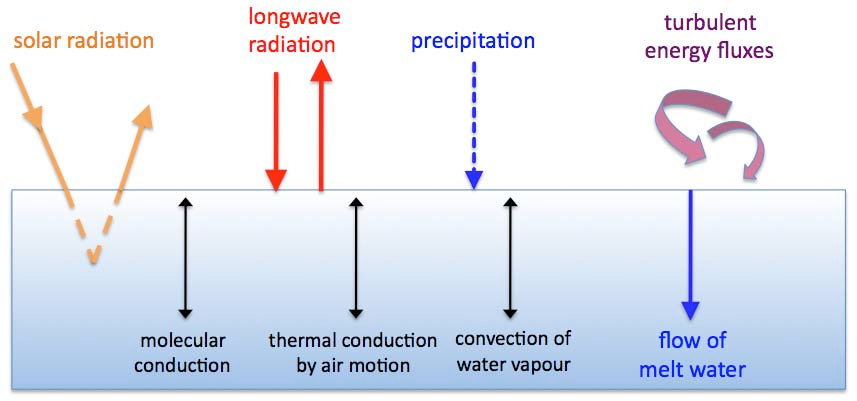
\includegraphics[width=0.8\textwidth]{pictures/energy_balance_components.png}
\caption[Energiebilanz Komponenten]{Energiebilanz Komponenten (Quelle: \cite{Themicroclimateofvalleyglaciers)}}
\label{fig:Energiebilanz Komponenten}
\end{figure}

Den größten Anteil am Energiefluss hat die Strahlungskomponente. Typischerweise liegt dieser Anteil bei ein paar Hundert Watt pro Quadratmeter. Je nach Beschaffenheit der Gletscheroberfläche wird mehr oder weniger dieser kurzwelligen Strahlung reflektiert. Der Prozentsatz, welcher angibt, wie viel Strahlung reflektiert wird, wird mit Albedo bezeichnet (siehe Kapitel \ref{Albedo}). Jener Teil, der nicht reflektiert wird, dringt in den Gletscher ein, wirkt sich also positiv auf die Energiebilanz aus(vgl. \cite[16]{Themicroclimateofvalleyglaciers}).\\

Langwellige Strahlung wird (fast) vollständig vom Gletscher absorbiert. Der Gletscher strahlt gleichzeitig aber auch langwellige Strahlung wieder ab. Bei warmen Temperaturen, hoher Luftfeuchtigkeit und Präsenz von Wolken, ist die Bilanz der langwelligen Strahlung positiv, ansonsten ist sie im Normalfall negativ.\\
Wolken führen nämlich dazu, dass weniger kurzwellige Sonnenstrahlung und mehr langwellige Strahlung zur Gletscheroberfläche gelangt. Für die Energiebilanz ist dabei aber noch wichtig zu wissen, ob der Gletscher eine hohe Albedo (z.B. Neuschnee) oder niedrige Albedo (z.B. Eis) aufweist. Eine hohe Albedo würde dazu führen, dass der Großteil an kurzwelliger Strahlung reflektiert wird. Nimmt also die Bewölkung zu, so gibt es mehr langwellige Strahlung die trotzdem absorbiert werden kann. Daraus resultiert eine positive Auswirkung auf die Energiebilanz.\\
Simultan dazu wirkt sich Bewölkung bei niedriger Albedo negativ auf die Energiebilanz aus. Der kurzwellige Strahlungseffekt würde dabei nämlich dem langwelligen überwiegen, da kurzwellige Strahlung energiereicher ist als langwellige(vgl. \cite[16, 17]{Themicroclimateofvalleyglaciers}).\\

Ob sich der Niederschlag positiv oder negativ auf die Energiebilanz des Gletschers auswirkt hängt von dessen Temperatur ab. Je nachdem, ob die Temperatur höher oder niedriger ist als die Gletscheroberflächentemperatur, ist die Auswirkung positiv oder negativ. Die Energieflüsse, welche hier wirken, sind aber sehr gering(vgl. \cite[17]{Themicroclimateofvalleyglaciers}).\\

Turbulente Energieflüsse zwischen der Gletscheroberfläche und der Atmosphäre wirken sich signifikant auf den Energiefluss aus. Grundvoraussetzung für diese turbulenten Energieflüsse ist eine Lufttemperatur über dem Gefrierpunkt. Grund dafür ist, dass die Energieflussrichtung im Gletscher dem Gradienten der Temperatur entspricht, was bedeutet, dass der Energiefluss in Richtung der Gletscheroberfläche verläuft. Je nach dem wie hoch die Lufttemperatur und Luftfeuchtigkeit sind, kann nun entweder durch Verdunstung Kälte oder durch Kondensation Wärme entstehen. Bei einer Lufttemperatur von $10^\circ C$ beispielsweise, stellt die relative Feuchtigkeit von $50~\%$ den Wendepunkt zwischen positiver ($>50~\%$) und negativer ($<50~\%$) Auswirkung auf die Energiebilanz dar(vgl. \cite[17]{Themicroclimateofvalleyglaciers}).\\

Der Fluss von Schmelzwasser innerhalb des Gletschers stellt einen latenten Wärmefluss dar. 
``Molecular conduction'' bezeichnet die Wärmeleitung durch Kollision von mikroskopisch kleinen Partikeln. Die Reibungshitze wirkt sich durch das Reiben des Eises an der Oberfläche ebenfalls positiv auf die Energiebilanz aus.\\
Kleine Energieflüsse entstehen auch noch aufgrund von Hitze- und Wasserdampftransport durch Konvektion im Schnee oder Firn. Diese Flüsse wirken sich aber vor allem auf die Metamorphose der Schneekristalle aus und sind abhängig von der Dichte des Schnees und vom Temperaturgradienten im Schnee (vgl. \cite[17]{Themicroclimateofvalleyglaciers}).


\subsubsection{Albedo}\label{Albedo}
Die Albedo bezeichnet das Verhältnis zwischen rückgestrahltem und einfallendem Licht. Sie gibt also den Prozentsatz an Strahlung an, der beispielsweise vom Gletscher reflektiert wird. Folgende Abbildung gibt einen Überblick über das Rückstrahlvermögen von verschiedenen Oberflächenbedeckungen eines Gletschers.

\begin{figure}[H]
\centering
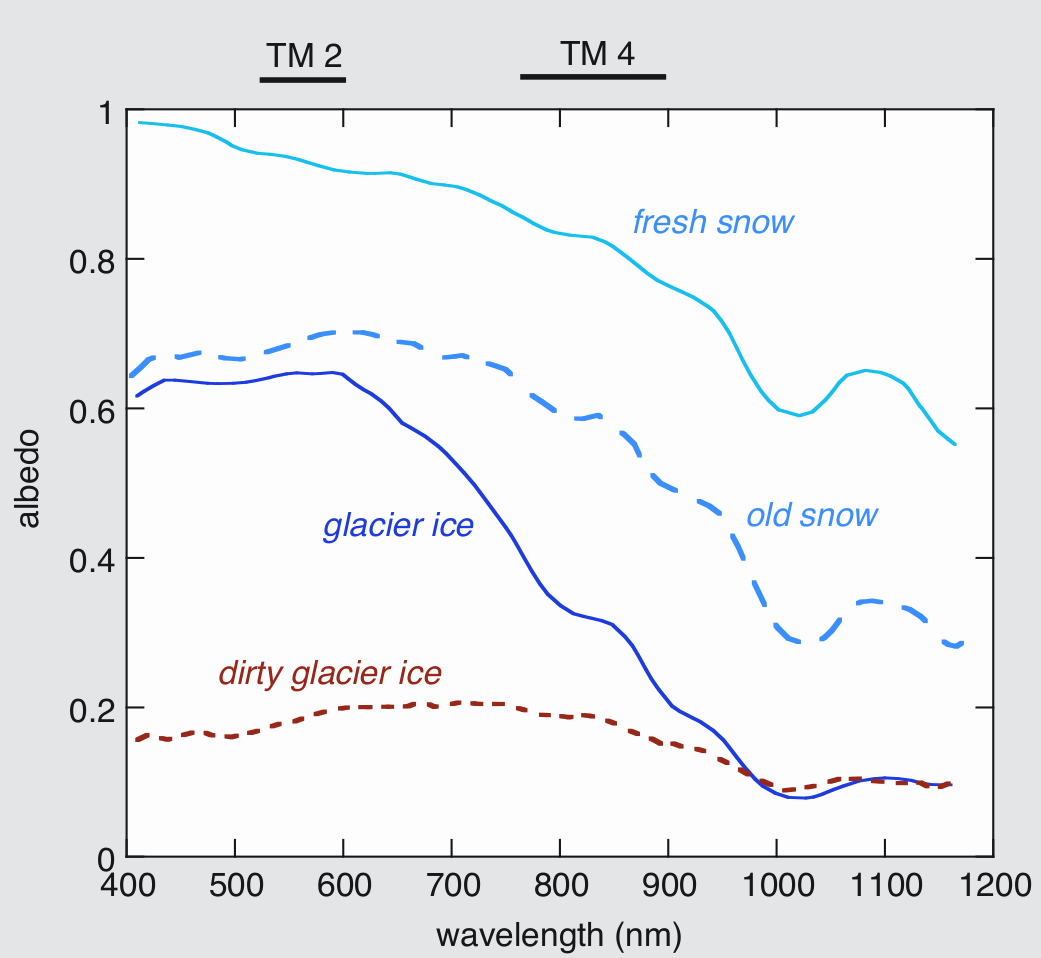
\includegraphics[width=0.63\textwidth]{pictures/spectral_reflectance_curves_for_ice_and_snow.png}
\caption[Spektrale Relektorkurven von Eis und Schnee]{Spektrale Relektorkurven von Eis und Schnee (Quelle: \cite{Themicroclimateofvalleyglaciers})}
\label{fig:Spektrale Relektorkurven von Eis und Schnee}
\end{figure}

Bei einem Gletscher verringert sich die Nettostrahlung, welche sich positiv auf die Energiebilanz des Gletschers auswirkt, mit zunehmender Höhe. Grund dafür ist eben genau die Albedo, denn Schnee bedeckt die höher liegenden Teile des Gletschers und reflektiert mehr Strahlung. Das Eis im Ablationsgebiet absorbiert sehr viel Strahlungsenergie, da hier die Albedo geringer ist. (vgl. \cite[171]{ThePhysicsOfGlaciers}).

\subsection{``global dimming'' und ``Global brigthening''}
Mehrere Langzeitstudien von Oberflächenstrahlungs-Messungen haben gezeigt, dass die Strahlung, welche auf der Erdoberfläche ankommt im Hinblick auf eine dekadische Zeit nicht konstant ist, d.h. sich innerhalb von 10er-Jahren signifikant ändern kann. Diese Änderungen wurden unter den Begriffen ``global dimming'' und ``global brightening'' (Globale Verdunkelung/Aufhellung) zusammengefasst, wobei der Begriff ``global'' sich auf die Summe von diffuser und direkter Sonnenstrahlung bezieht und nicht auf global, im Sinne von ``auf der ganzen Welt''.\\
Änderungen der Oberflächenstrahlung können nicht nur bei wolkigen Bedingungen festgestellt werden, sondern auch bei einer wolkenfreien Atmosphäre. Das deutet darauf hin, dass sich anthropogene Einflüsse (z.B. das Einbringen von Aerosolen in die Atmosphäre) auf diese Oberflächenstrahlung auswirken (vgl. \cite[1]{GlobalDimming}).\\
Aerosole können diese Oberflächenstrahlung verändern indem sie die Sonnenstrahlen streuen oder absorbieren. Weiters können die Aerosole als Kondensationskerne bei der Wolkenbildung agieren und somit diese fördern. Insgesamt reduzieren also Aerosole die Oberflächenstrahlung. Eine der Hauptursachen von ``global dimming'' ist somit die Erzeugung von Aerosolen durch die Industrie (vgl. \cite[14]{GlobalDimming}).\\ 
Die Oberflächenstrahlung bzw. die kurzwellige Sonnenstrahlung spielt, wie bereits in Kapitel \ref{Energiebilanz Komponenten} erwähnt, eine große Rolle in der Energiebilanz der Gletscher. Auf der Nordhalbkugel sei zu beobachten gewesen, dass bis zu den 1980-Jahren keine signifikanten Änderungen in den Flächenbedeckungen der Gletscher stattgefunden hat, aber ab ca. 1980 mit dem Effekt des ``global brigthening'' die Gletscher schlagartig an Größe verloren hätten (vgl. \cite[24]{GlobalDimming}). Zwischen $-3$ und $-9$ $W/m^2$ wird von ``global dimming'' gesprochen, von $+1$ bis $+4$ $W/m^2$ von ``global brightening'' (vgl. \cite[28]{EnlighteningGlobalDimming}).


\pagebreak
\section{Methodik}
\subsection{Berechnung der Energiebilanz}
Um das Ziel der Arbeit zu erreichen, muss die Energiebilanz eines Gletschers errechnet werden. \citeauthor{ThePhysicsOfGlaciers} (\citeyear{ThePhysicsOfGlaciers}) geben in Kapitel 5 ``Mass Balance Processes: 2. Surface Ablation and Energy Budget'' detaillierte Formeln zur Berechnung der Energiebilanz an. Ausgegangen wird von Formel 

\begin{equation}
E_{N}=\underbrace{E_{S}^{\downarrow}+E_{S}^{\uparrow}+E_{L}^{\downarrow}+E_{L}^{\uparrow}}_{E_{\mathrm{R}}}+E_{G}+E_{H}+E_{E}+E_{P},
\end{equation}

wobei $E_{N}$ dem Nettoenergiefluss in die Oberfläche, $E_{S}^{\downarrow}$ der ankommenden kurzwelligen Strahlung, $E_{S}^{\uparrow}$ der reflektierten kurzwelligen Strahlung, $E_{L}^{\downarrow}$ der ankommenden langwelligen Strahlung, $E_{L}^{\uparrow}$ der reflektierten langwelligen Strahlung $E_{G}$ dem Energiefluss unter der Oberfläche, $E_{P}$ dem Energieeintrag durch Niederschlag und $E_{H}$ und $E_{E}$ den spürbaren und latenten Wärmeflüssen durch Zirkulation entsprechen. $E_{\mathrm{R}}$ ist die Summe aller Strahlungen und gibt somit die Nettostrahlung an (positiv für Energieeintrag in den Gletscher).\\

Ausgehend von dieser Grundgleichung beschreiben \citeauthor{ThePhysicsOfGlaciers} weitere Aspekte die zu berücksichtigen sind, wie zum Beispiel 

\begin{itemize}
\item{Schmelzrate, abhängig auch von Dicke }
\item{Wiedergefrieren von Schmelzwasser in den unteren Schichten erzeugt Wärme}
\item{Abhängigkeit der kurzwelligen Strahlung vom Einfallswinkel und von der atmosphärischen Durchlassungsfähigkeit}
\end{itemize}

Um die spürbaren und latenten Wärmeflüsse $E_{H}$ und $E_{E}$ zu berechnen, schildern \citeauthor{ThePhysicsOfGlaciers} eine Berechnungsmethode über den ``Bulk Aerodynamic Approach'' und die ``Flux-gradient Theory'' (vgl. \cite[153-157]{ThePhysicsOfGlaciers}).\\
Die genaue Herleitung dieser Formeln kann dort nachgelesen werden, als Ergebnis folgen schlussendlich aber die zwei Formeln

\begin{equation}\label{eq:Berechnung latenter Energiefluss}
E_{E}= 22.2~C^*~\mu(z)~(e_a-e_s)
\end{equation}

für den latenten und

\begin{equation}\label{eq:Berechnung sensibler Energiefluss}
E_{H}= 0.0129~C^*~P~\mu(z)~(T_a(z)-T_s)
\end{equation}

für den sensiblen Wärmefluss. $C^*$ ist dabei der Transfer-Koeffizient und wird mit 

\begin{equation}\label{eq:Transfer-Koeffizient}
C^{*}=\frac{k_{o}^{2}}{\ln ^{2}\left(z / z_{0}\right)}
\end{equation}

% TODO Pfad
berechnet, wobei $k_{o}=0.4$ die Karmans Konstante ist, $z_{0}$ die Messhöhe über dem Eis ist, in welcher die Windgeschwindigkeit gemessen wird und $z=0.003~m$ dem Rauheitsparameter entspricht. Tabelle 5.4 in \citeauthor{ThePhysicsOfGlaciers} (\citeyear[155]{ThePhysicsOfGlaciers}) zeigt, dass dieser Parameter bei Eis im Ablationsgebiet zwischen 1 und 5 Millimetern liegt. Deshalb wird er in den Berechnungen hier mit dem Mittelwert 3 Millimeter angenommen.\\ % evtl footnote bei Karmans Konstante TODO?

$T_s$ entspricht der Oberflächentemperatur des Eises und wird mithilfe vom Stefan-Boltzmann-Gesetz 

\begin{equation}\label{eq:Boltzmann-Gesetz}
I = e \cdot \sigma \cdot T^4
\end{equation}

% TODO braucht es Nachweis, dass diese 1 ist ca.?
berechnet. $e$ entspricht der Emissivität, welche bei Eis im Infrarotbereicht ungefähr 1 ist. $\sigma=5.670 \cdot 10^{-8}$ entspricht der Stefan-Boltzmann-Konstante und $T$ der Oberflächentemperatur des Körpers. $I$ ist die abgestrahlte Energie in $W/m^2$ welche hier in Form der langwelligen Ausstrahlung gegeben ist. Somit folgt durch Umstellungen die Oberflächentemperatur

\begin{equation}\label{eq:Oberflächentemperatur}
T = \sqrt[4]{\frac{I}{\sigma}}
\end{equation}


$e_a$ entspricht dem tatsächlichen Wasserdampfdruck in der Luft und wird aus dem Sättigungswasserdampfdruck


\begin{equation}
e_{a_{saturated}}=0.6108 \cdot e^{17.27 \cdot \frac{T_a}{T_a + 237.3}}
\end{equation}

durch

\begin{equation}
e_a = \frac{rel_{humidty}}{100} \cdot e_{a_{saturated}}
\end{equation}

berechnet. $T_a$ entspricht dabei der Lufttemperatur in Grad Celsius und die Einheit des Ergebnisses $e_a$ ist $kPa$.\\

$e_s$ wird analog zu $e_a$ berechnet, nur dass statt der Lufttemperatur $T_a$ die mit Formel \ref{eq:Oberflächentemperatur} berechnete Eisoberflächentemperatur verwendet wird.\\
$\mu(z)$ und $T_a(z)$ stehen für die Windgeschwindigkeit und Lufttemperatur gemessen in Höhe $z$, $P$ für den Luftdruck in Einheit Pascal.


\subsection{Periodische Trendelimination}\label{Periodische Trendelimination}
Im Falle der Pasterze stehen nur für 3 Jahre Messdaten für die Berechnung der Energiebilanz zur Verfügung. Deshalb kann durch eine periodische Trendelimination keine aussagekräftige Annahme über einen eventuellen Trend getroffen werden. Trotzdem wird die Möglichkeit zur periodischen Trendelimination in die Software implementiert, um z.B. bei anderen Gletschern und längeren Datenaufzeichnungen bzw. in Zukunft auch bei der Pasterze Trendanalysen durchführen zu können.\\

Eine Periode dauert bei der Energiebilanz genau ein Jahr. Die Bereinigung von der Periode erfolgt auf die Weise, dass der erste Wert nach dem vollendeten Jahr vom Wert im ersten Jahr zu dieser Zeit abgezogen wird. Es wird dabei immer jener Wert vom ersten Jahr gesucht, welcher datumsmäßig (abzüglich von der Jahresanzahl) am nächsten zum betrachteten Wert liegt. Dieser Vorgang wird für alle weiteren Werte wiederholt. Soll ein eventueller linearer Trend erhalten bleiben, so müssen die Werte immer bezogen auf das erste Jahr abgezogen werden. Wird nämlich immer nur das Vorjahr herangezogen, so fällt dieser lineare Trend auch noch weg. In diesem Fall könnten dann die entstandenen Residuen auf Normalverteilung überprüft werden.\\
Bei dieser Trendelimination soll aber der lineare Trend eben aufrecht erhalten bleiben. Aufgrund der genannten Methode folgt somit, dass die Wertereihe zumindest größer als ein Jahr sein muss, ansonsten kann kein periodischer Trend eliminiert werden.\\

Im Zuge der Durchführung wird nicht nur die errechnete Energiebilanz an sich trendeliminiert, sondern auch Einzelteile, wie z.B. nur die Strahlungsenergie oder nur der sensible und latente Wärmeeintrag.


\subsection{Berechnung des resultierenden Schmelzwassers}\label{Section Berechnung Schmelzwasser}
Formel (vgl. \cite[142]{ThePhysicsOfGlaciers})

\begin{equation}
\rho_{w} L_{f} \dot{m}_{s}\left[1-f_{r}\right]+\int_{0}^{\Delta z} \rho c \frac{\partial T}{\partial t} d z=E_{N}
\end{equation}


gibt einen Zusammenhang zwischen Nettoenergiebilanz und der Schmelzrate $\dot{m}$ vom Gletschereis. Wenn die Temperatur im betrachteten Eislayer den Schmelzpunkt erreicht hat, dann fällt der zweite Term der Gleichung durch


\begin{equation}
\int_{0}^{\Delta z} \rho c \frac{\partial T}{\partial t} d z=0
\end{equation}

weg. Um die errechnete Energiebilanz auf Plausibilität zu überprüfen, indem die gemessene Ablation (später umgerechnet in Schmelzwasser) mit dem modellierten Schmelzwasser verglichen wird, reicht es für diese Analyse aus, nur den Zeitraum von 1. Juni bis 1. September zu betrachten. In diesem Zeitraum kann nämlich von einem isothermen Eislayer mit Temperatur um den Schmelzpunkt ausgegangen werden.

$f_r$ bezeichnet den Anteil vom Schmelzwasser, der im Eislayer wiedergefriert. Es folgt somit die für diese Fragestellung relevante Nettoablationsrate 

\begin{equation}
\dot{m}_{s}\left[1-f_{r}\right]=E_{N} / \rho_{w} L_{f},
\end{equation}

wobei $\rho_{w}=1000~kg/m^{3}$ der Wasserdichte bei $0^\circ C$ und $L_{f}=3.34 \cdot 10^5 J/kg$ der latenten Schmelzwärme von purem Eis bei $0^\circ C$ entspricht (vgl. \cite[142]{ThePhysicsOfGlaciers}).

Die errechnete Nettoablationsrate hat die Einheit $m^3/\Delta T$, mit

\begin{equation}
W = \dot{m}_{s}\left[1-f_{r}\right] \cdot \Delta T \cdot 1000
\end{equation}


folgt somit das tatsächliche Schmelzwasser in Liter über einen gewissen Zeitraum $\Delta T$.

Durch 

\begin{equation}
a_{meas} = W \cdot \rho_{i}
\end{equation}


kann die gemessene Ablation in Metern ebenfalls in Schmelzwasseräquivalent umgerechnet werden. $\rho_{w}=917~kg/m^3$ steht dabei für die Dichte von purem Eis bei $0^\circ C$.\\

Analog dazu kann auch das modellierte Schmelzwasser durch

\begin{equation}
a_{mod} = -\frac{W}{\rho_{i}}
\end{equation}

noch in Ablation in Metern umgerechnet werden.

\subsection{Bereinigung der Ablationsmessung}
Die Ablation wird bei der Pasterze mit einem Druck-Transducer gemessen. Dieser misst den Druckunterschied zwischen Sensor und Eisoberfläche. Der Sensor schmilzt allerdings von Zeit zu Zeit gänzlich aus und muss wieder neu positioniert werden. Dies hat zur Folge, dass in den Messdaten Sprünge sind. Um diese Sprünge softwareseitig zu bereinigen, wird darauf abgefragt, ob sich die gemessene Ablation von einem auf den nächsten Schritt über einen gewissen Threshold-Wert vergrößert. Dieser Grenzwert ist in der Software mit $10~cm$ bei einer Messauflösung von 10 Minuten angenommen. Die Differenz des Sprunges wird dann bei den folgenden Messungen angebracht um so eine stetig abnehmende Kurve zu generieren.



\subsection{Programmierung in Python}
\subsubsection{Umgebung}

Die entwickelte Software wurde im Programm Pycharm Professional Edition objektorientiert geschrieben. Die verwendete Python Version ist Python 3.6.\\\\
Die verwendeten Module und deren Zweck in der Software werden in folgender Tabelle erklärt:


\begin{table}[H]
\centering
\setstretch{1.3} 
\caption{Python Module mit Erklärung}
\label{tab:Python Module}
\begin{tabular}{|l|l|}
\hline
\textbf{Modul} & \textbf{Zweck}                                \\ \hline
tkinter             & Erstellung des GUI         \\
os             & Ordnerverwaltung         \\
configparser             & Verwaltung der Konfigurationsdatei         \\
numpy          & Erstellung und Handhabung von Arrays          \\
matplotlib     & Grafische Darstellung der Daten               \\
math		   & Berechnungsfunktionen (Logarithmus, Wurzel, e-Funktion, ..)   \\  
datetime		   & Verwaltung von Zeit und Datum   \\
unittest		   & Erstellung einer Testumgebung   \\  
pyinstaller		   & Erstellung der .exe für Windows   \\ \hline


\end{tabular}
\end{table}
%setstretch is removed automatically after table again
\vspace{0.3cm}

\subsubsection{``Unittesting''}
Das Python Modul unittest wird dazu verwendet, Funktionen des Programmes zu überprüfen. In dieser Arbeit wird es dazu verwendet, die Richtigkeit der Formeln für die Berechnung der Energiebilanz zu gewährleisten.\\

\citeauthor{ThePhysicsOfGlaciers} (\citeyear[157]{ThePhysicsOfGlaciers}) bieten Testwerte und das dazugehörige Ergebnis für den Transfer-Koeffizienten $C^*$ von Formel \ref{eq:Transfer-Koeffizient} und für die Berechnungen der sensiblen Wärme Formel \ref{eq:Berechnung sensibler Energiefluss} an.


\paragraph{Transfer-Koeffizient}

Bei gegebener Messhöhe zwischen 1 und 2 Metern und Oberflächenrauheit von  1 - 5 Millimetern (entspricht der Oberflächenrauheit von Eis im Ablationsgebiet, Tabelle 5.4) soll ein Wert für den Transfer-Koeffizienten (Formel \ref{eq:Transfer-Koeffizient}) zwischen 0.002 und 0.004 herauskommen.\\

Der Test mit einer Messhöhe von 1.5 Metern und Oberflächenrauheit von 2 Millimetern wird angenommen.

\paragraph{Sensible Wärme}
Bei gegebenem Luftdruck von $800~hPa$, Windgeschwindigkeit von $5~m/s$, Lufttemperatur von $5^\circ C$ und Transfer-Koeffizienten von $0.002$ soll das Ergebnis der sensiblen Wärme (Formel \ref{eq:Berechnung sensibler Energiefluss}) zwischen 47 und $53~W/m^2$ liegen. \\
Weiters erwähnt ist, dass von einer schmelzenden Eisoberfläche ausgegangen wird und da die Eisoberflächentemperatur nach Stefan Boltzmann (Formel \ref{eq:Boltzmann-Gesetz}) berechnet wird, wird der Funktion als langwellige Ausstrahlung ein Wert von $1000~W/m^2$ mitgegeben, womit die Eistemperatur in der Berechnung bei 0 liegt.\\

Der Test wird wiederum angenommen.

\subsubsection{Grafisches Userinterface}
Das Grafische Userinterface (GUI) setzt sich aus den Teilen 
\begin{itemize}
\item Read
\item Scope/Energy balance
\item Sum
\item Plot
\item Download
\end{itemize}
zusammen.\\

In \textbf{Read} kann eine Messdatei eingelesen werden. 

\begin{figure}[H]
\centering
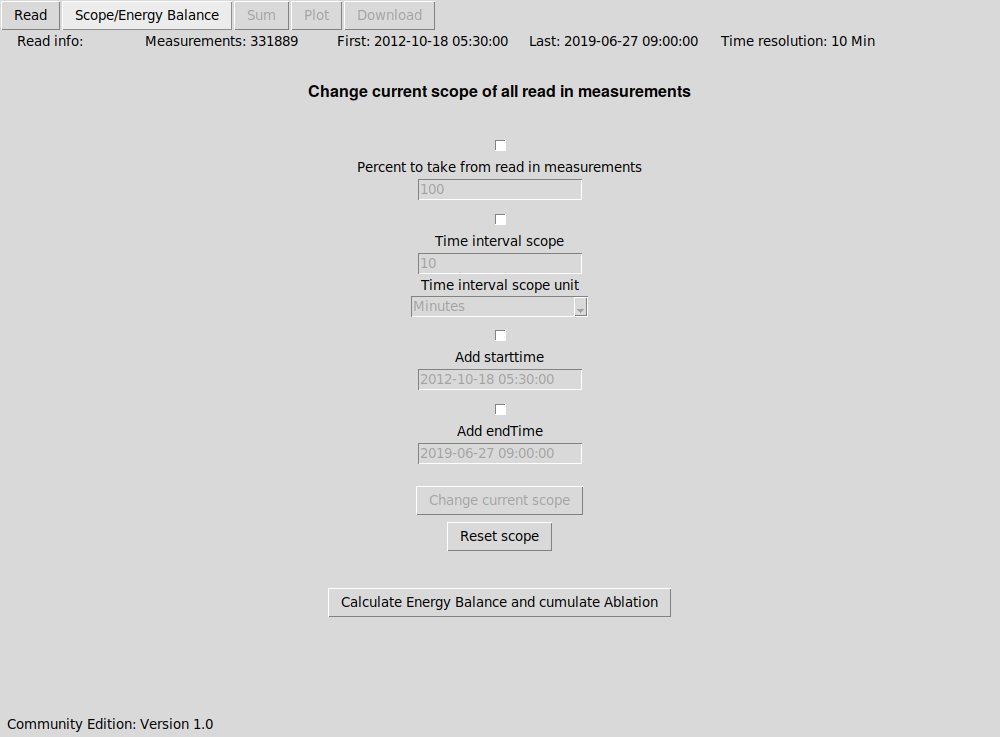
\includegraphics[width=\guiplotsize\textwidth]{pictures/GUI/Read_Frame.png}
\caption[GUI Read-Frame, Version \guiversion]{GUI Read-Frame, Version \guiversion, (Quelle: eigene Darstellung)}
\label{fig:GUI Read-Frame}
\end{figure}

Im Fenster \textbf{Scope/Energy balance} kann der momentane Betrachungszeitraum verändert werden und die Energiebilanz berechnet werden. 

\begin{figure}[H]
\centering
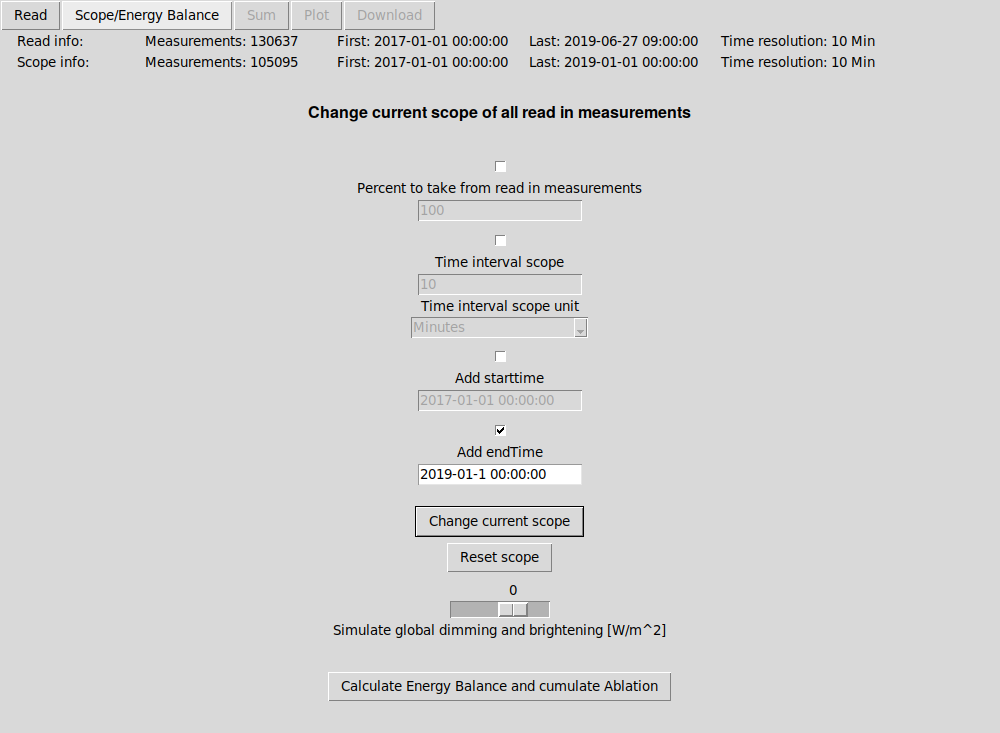
\includegraphics[width=\guiplotsize\textwidth]{pictures/GUI/Scope_Energy_Balance_Frame.png}
\caption[GUI Scope/Energy Balance-Frame, Version \guiversion]{GUI Scope/Energy Balance-Frame, Version \guiversion, (Quelle: eigene Darstellung)}
\label{fig:GUI Scope/Energy Balance-Frame}
\end{figure}

Bei \textbf{Sum} können einzelne Messungen zusammengefasst werden.

\begin{figure}[H]
\centering
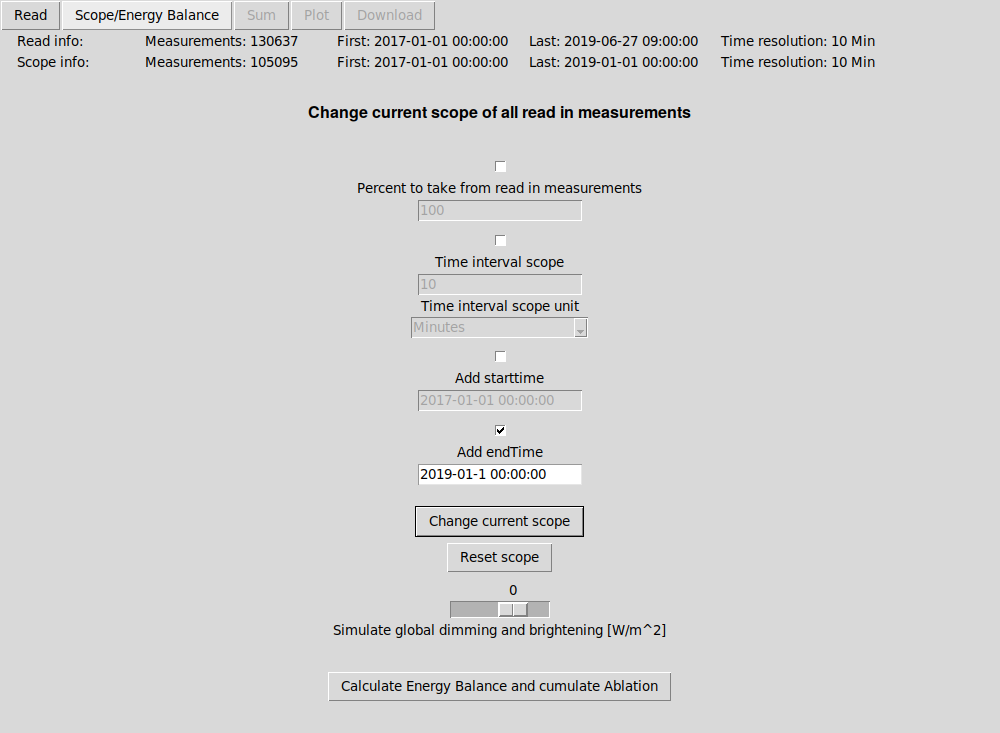
\includegraphics[width=\guiplotsize\textwidth]{pictures/GUI/Scope_Energy_Balance_Frame.png}
\caption[GUI Sum-Frame, Version \guiversion]{GUI Sum-Frame, Version \guiversion, (Quelle: eigene Darstellung)}
\label{fig:GUI Sum-Frame}
\end{figure}

In \textbf{Plot} können die Ergebnisse als graphische Darstellungen betrachtet werden. Es ist dabei möglich, die gesamte Energiebilanz sowie deren Einzelteile zu plotten. Weiters kann die Ablation oder die errechnete gemessene und modellierte Eisschmelze als zweite Achse eingeblendet werden. Auch die Trendelimination kann visualisiert werden.

\begin{figure}[H]
\centering
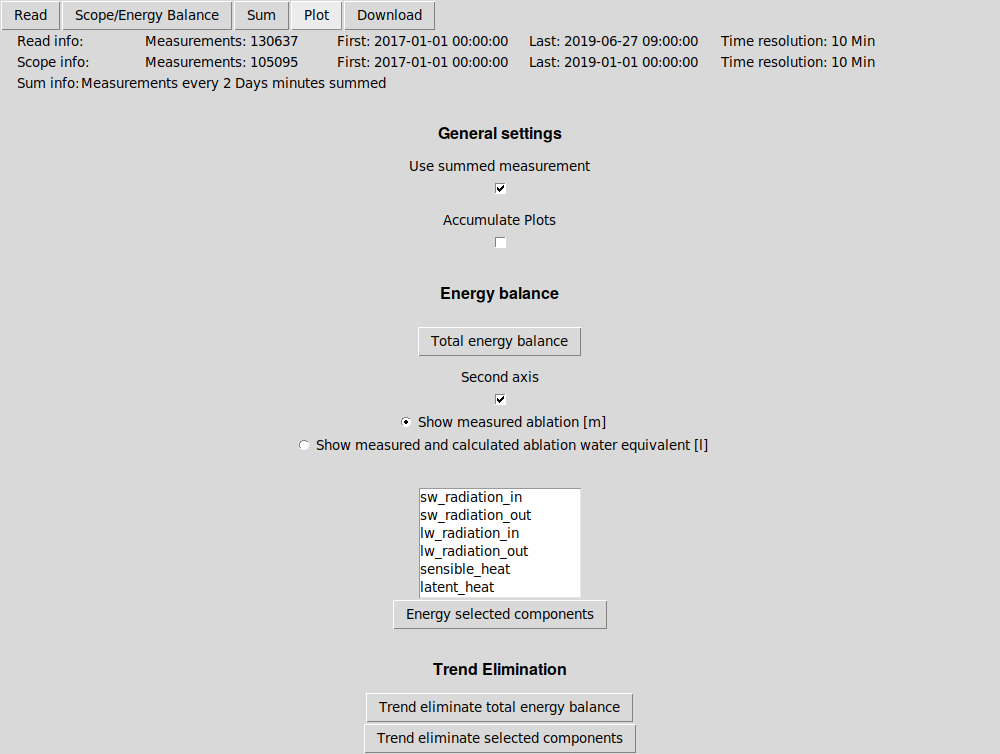
\includegraphics[width=\guiplotsize\textwidth]{pictures/GUI/Plot_Frame.png}
\caption[GUI Plot-Frame, Version \guiversion]{GUI Plot-Frame, Version \guiversion, (Quelle: eigene Darstellung)}
\label{fig:GUI Plot-Frame}
\end{figure}

Beim erstellen des Plots erscheint ein neues Fenster, in welchem der Plot vergrößert bzw. verkleinert, verschoben und heruntergeladen werden kann.

\begin{figure}[H]
\centering
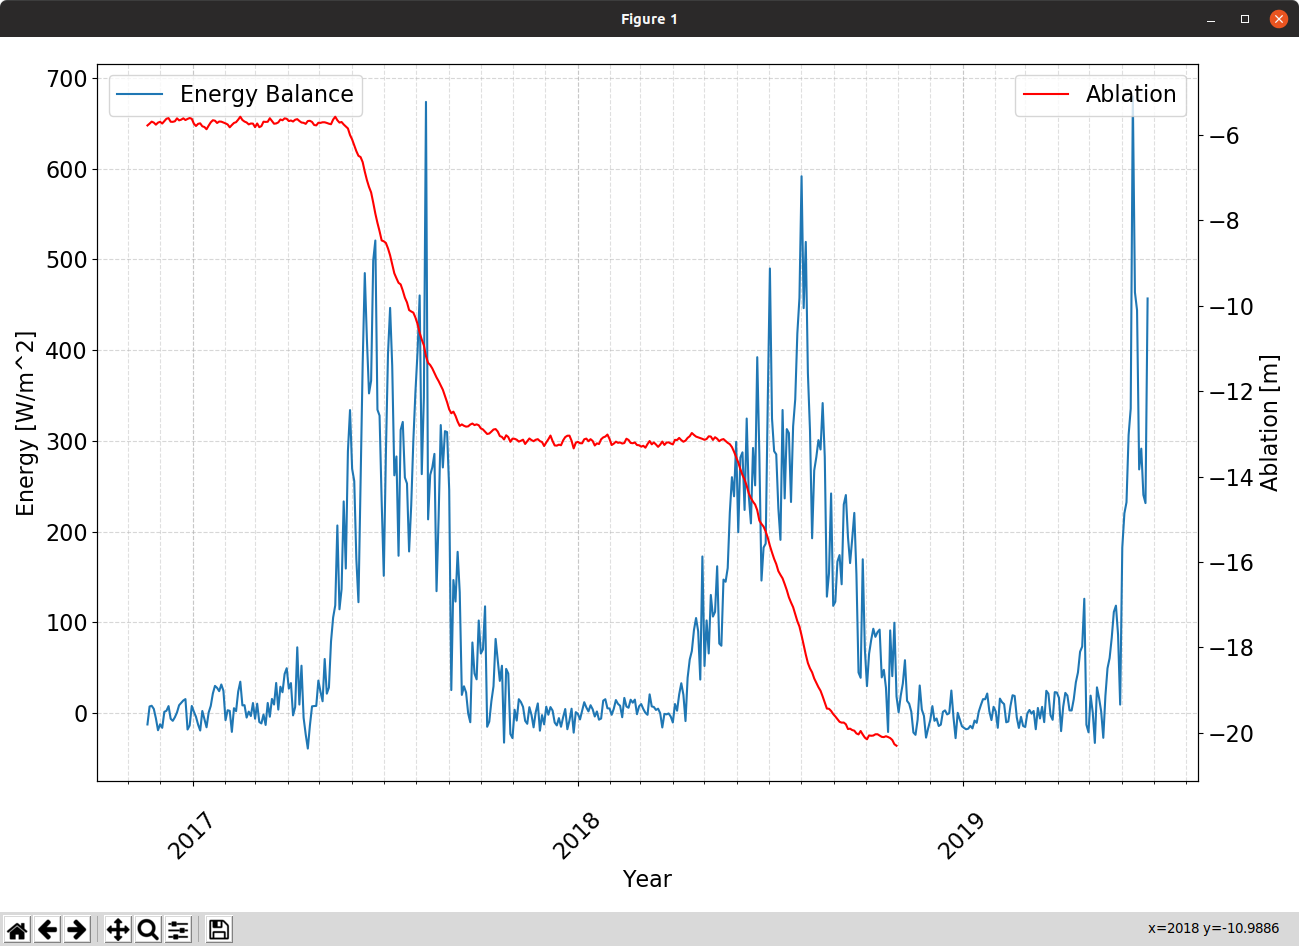
\includegraphics[width=\guiplotsize\textwidth]{pictures/GUI/Sample_Plot.png}
\caption[GUI Beispiel Plot]{GUI Beispiel Plot (Quelle: eigene Darstellung)}
\label{fig:GUI Beispiel Plot}
\end{figure}

Im \textbf{Download}-Bereich können die erzielten Ergebnisse noch in Form von Wertetabellen heruntergeladen werden.

\begin{figure}[H]
\centering
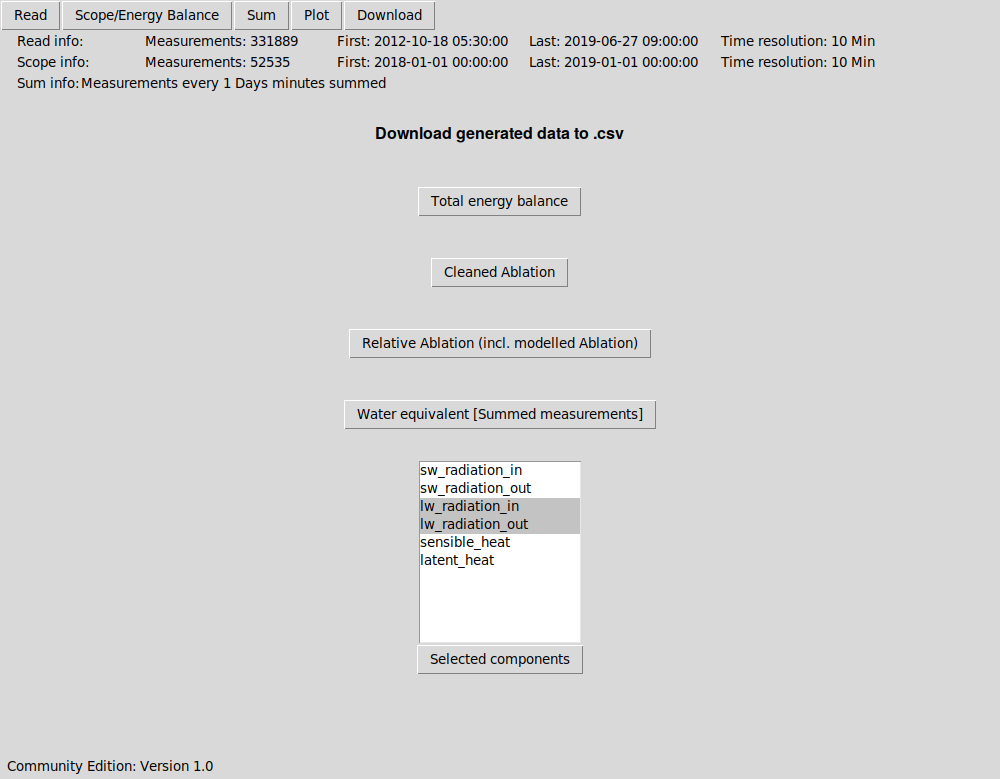
\includegraphics[width=\guiplotsize\textwidth]{pictures/GUI/Download_Frame.png}
\caption[GUI Download-Frame, Version \guiversion]{GUI Download-Frame, Version \guiversion, (Quelle: eigene Darstellung)}
\label{fig:GUI Download-Frame}
\end{figure}

Eine detaillierte Beschreibung des GUI befindet sich unter

\textsf{\small https://bitbucket.org/atraxoo/energiebilanzablationsgebietpasterze/wiki/Home}
 im Wiki des Projektes auf der Plattform Bitbucket.


\subsection{Softwareverwaltung}
\subsubsection{Download und Installation}
Die Open Source Version der Software ist öffentlich auf der  Platform Bitbucket unter dem Namen EnergiebilanzAblationsgebietPasterze zugänglich. Mit Klick auf Clone erscheint ein Text, der kopiert und im Terminal im gewünschten Verzeichnis ausgeführt werden muss. Git muss dafür am Rechner installiert sein.\\

Beispiel:

Terminal: \textsf{\small git clone git@bitbucket.org:atraxoo/energiebilanzablationsgebietpasterze.git}\\


Es wird nun die gesamte Software, inklusive einer Messdaten Beispieldatei, heruntergeladen. Weiters wird ein Verzeichnis Exe heruntergeladen, in dem sich eine ausführbare .exe Datei befindet, womit das Programm unter Windows direkt und ohne Installation von Python ausgeführt werden kann.\\

Empfehlenswerter, vor allem im Bezug auf Updates, ist es allerdings, die Software direkt mit Python auszuführen. Dafür muss Python 3.6 oder Python 3.7 am Rechner installiert sein. Für die richtige Funktion der Software müssen gewisse Python Module installiert werden, welche sich in der requirements.txt Datei befinden. Diese Pakete können automatisiert mit dem Befehl\\

Windows Terminal: \textsf{\small pip install -r requirements.txt}\\
Linux Terminal:  \textsf{\small pip3 install -r requirements.txt}\\

installiert werden.

Optional aber empfehlenswert ist außerdem die Verwendung einer virtual environment in Python. In der offiziellen Python Dokumentation unter \textsf{\small https://docs.python.org/3/library/venv.html} ist eine Erklärung dazu zu finden.

Nachdem die Module installiert wurden, kann die Software mit \\

Windows Terminal: \textsf{\small python main.py}\\
Linux Terminal: \textsf{\small python3 main.py}\\

gestartet werden.

\subsubsection{Update}
Die aktuellste Version der Open Source Version kann mit \\

Terminal: \textsf{\small git pull} (Im Software Verzeichnis)\\

heruntergeladen werden. Zur direkt ausführbaren .exe Version gibt es keine Updates.

\pagebreak
\section{Ergebnisse und Interpretation}
\subsection{Energiebilanz}
Abbildung \ref{fig:Energiebilanz gesamter Messzeitraum, Zeitintervall 10 Minuten} zeigt die errechnete Energiebilanz über den gesamten Zeitraum in welchem Messdaten vorhanden sind (Ende 2016 bis Mitte 2019). 

\begin{figure}[H]
\centering
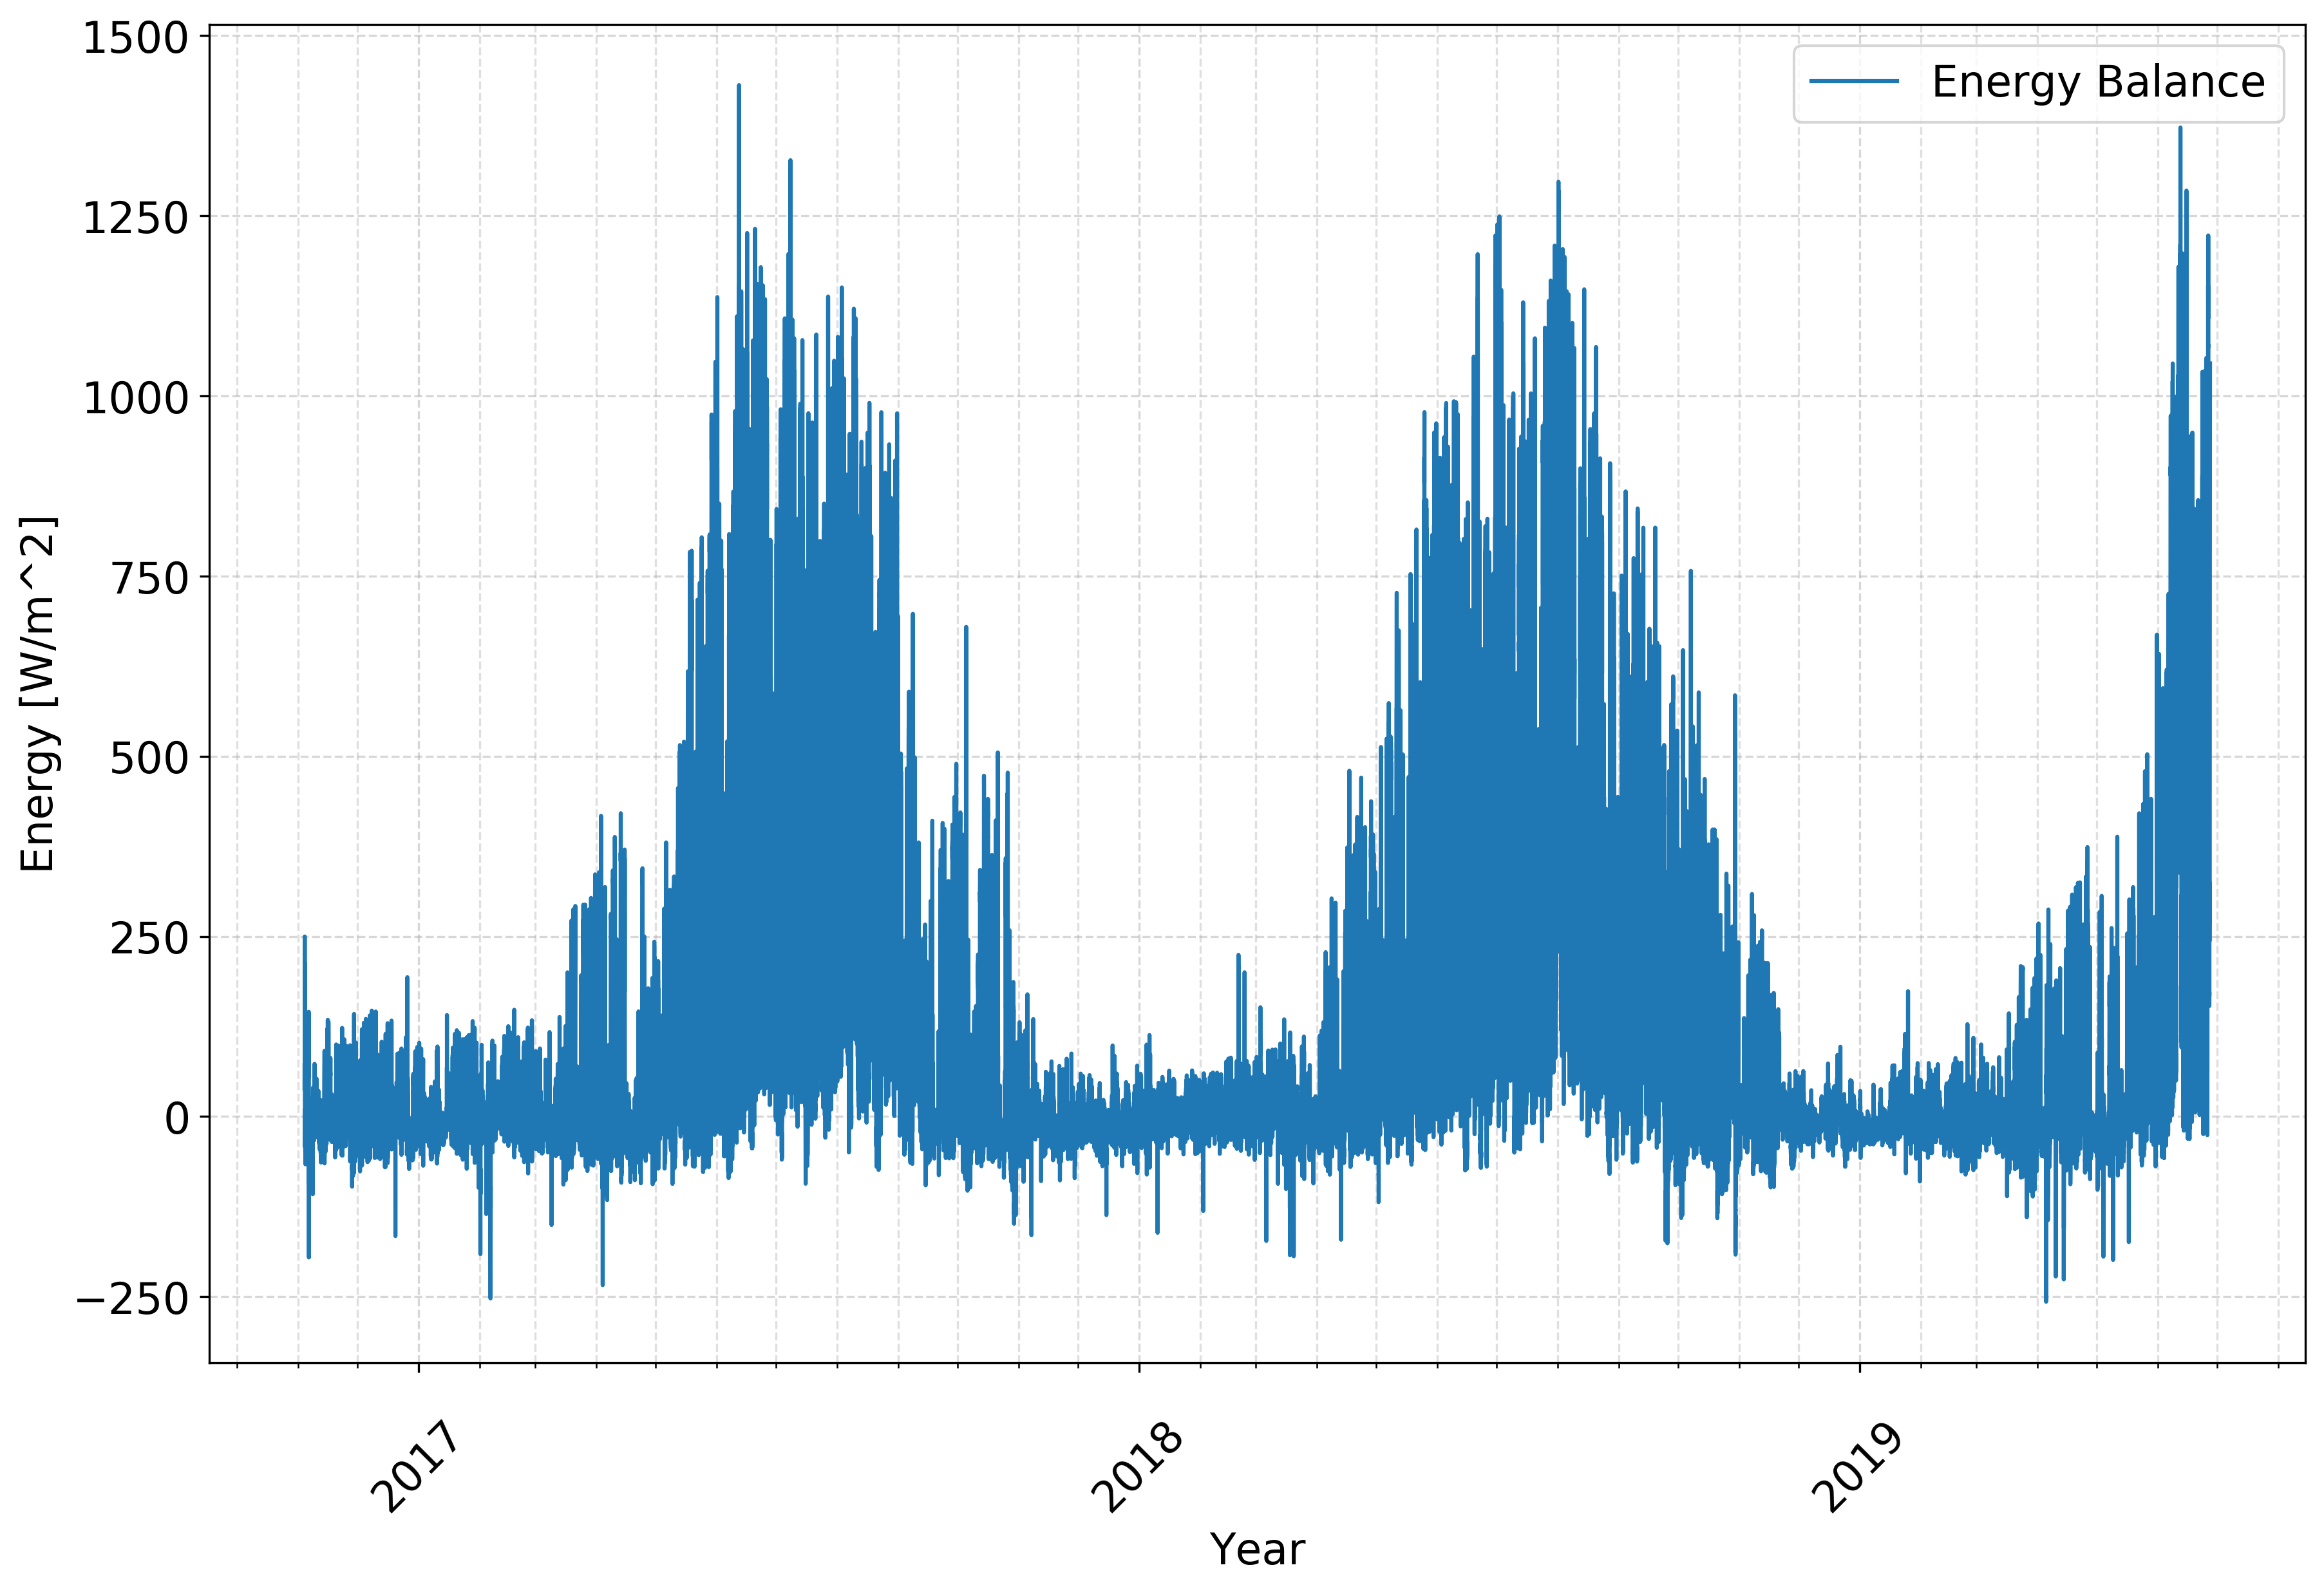
\includegraphics[width=\resultplotsize\textwidth]{../Software/plots/Total_energy_balance.png}
\caption[Energiebilanz, Ablationsgebiet Pasterze im Zeitraum November 2016 bis Juni 2019, Zeitintervall 10 Minuten]{Energiebilanz, Ablationsgebiet Pasterze im Zeitraum November 2016 bis Juni 2019, Zeitintervall 10 Minuten (Quelle: eigene Darstellung)}
\label{fig:Energiebilanz gesamter Messzeitraum, Zeitintervall 10 Minuten}
\end{figure}

Es sind nur knapp drei Jahre ausreichend Messdaten zur Berechnung der Energiebilanz verfügbar. An den Daten ist deutlich ein periodischer Verlauf erkennbar mit Maxima im Sommer und Minima im Winter. Die Spitzen der Energiebilanz liegen bei knapp 1500 $W/m^2$, die Minima bei ca. $-250 W/m^2$. Diese ungleiche Verteilung ist erklärbar durch die Messungen im Ablationsgebiet des Gletschers. Hier sollte ja das Jahresmittel deutlich positiv sein. Folgende Tabelle zeigt einen Überblick der Energiebilanz in den Jahren 2017 und 2018. Weiters werden in der darauf folgenden Abbildung \ref{Energiebilanzkomponenten Monatsmittel} die einzelnen Komponenten der Energiebilanz monatlich gemittelt dargestellt.

\begin{table}[H]
\centering
\setstretch{1.3} 
\caption{Energiebilanz Mittel (Einheit $W/m^2$)}
\label{tab:Energiebilanz Mittel}
\begin{tabular}{|l|cc|cc|cc|}
\hline
     & \multicolumn{2}{c|}{\textbf{Strahlungskomp}.} & \multicolumn{2}{c|}{\textbf{Sensible/Latente Wärme}} & \multicolumn{2}{c|}{\textbf{Gesamtenergiebilanz}} \\ \hline
Jahr & Jun-Aug           & Gesamt           & Jun-Aug               & Gesamt              & Jun-Aug         & Gesamt                 \\ \hline
2017 & 62.5              & 42.4             & 79.5                  & 58.1                & 142.0           & \textbf{100.4}         \\ \hline
2018 & 49.8              & 48.2             & 64.2                  & 60.9                & 114.0           & \textbf{109.1}         \\ \hline
\end{tabular}
\end{table}


\begin{figure}[H]
\centering
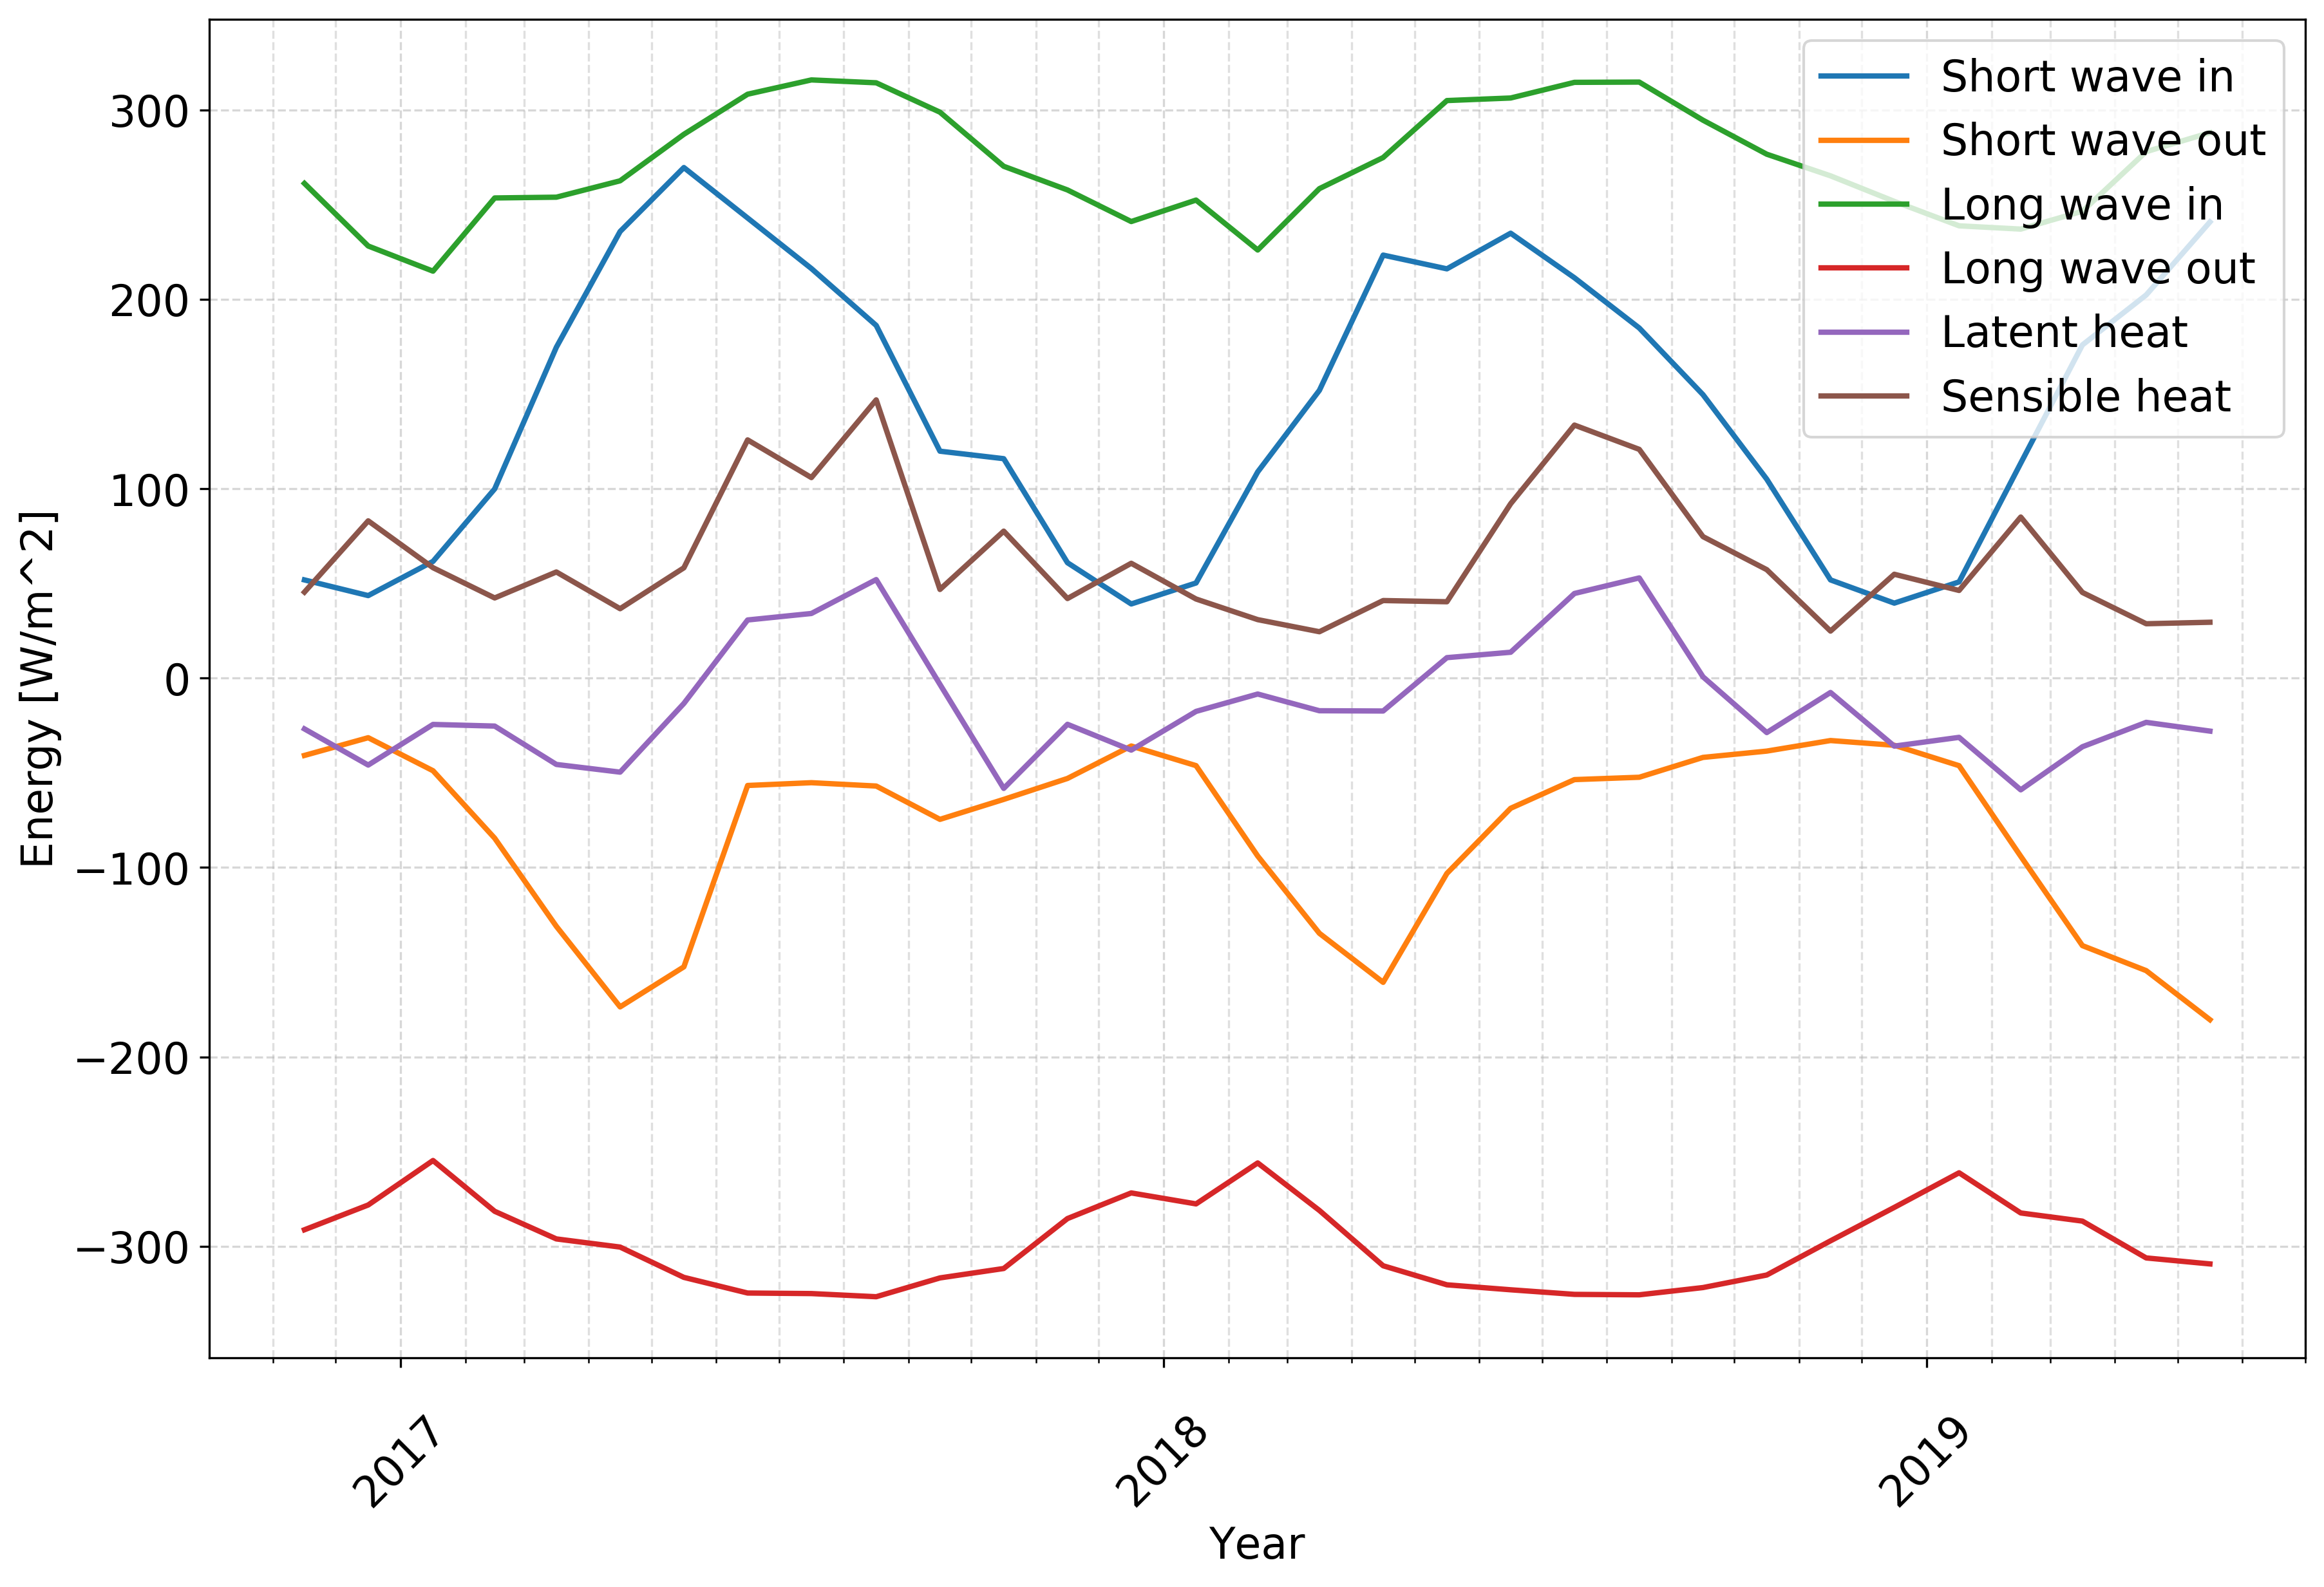
\includegraphics[width=\resultplotsize\textwidth]{../Software/plots/Energy_balance_components_monthly_mean.png}
\caption[Energiebilanzkomponenten Monatsmittel, Ablationsgebiet Pasterze im Zeitraum November 2016 bis Juni 2019]{Energiebilanzkomponenten Monatsmittel, Ablationsgebiet Pasterze im Zeitraum November 2016 bis Juni 2019 (Quelle: eigene Darstellung)}
\label{Energiebilanzkomponenten Monatsmittel}
\end{figure}

Der stärkste periodische Trend ist bei der eintreffenden kurzwelligen Strahlung zu erkennen. Den größten positiven Energieeintrag stellt allerdings die eintreffende langwellige  Strahlung dar. Generell lässt sich feststellen, dass die langwelligen Strahlungskomponenten einen geringeren periodischen Trend aufweisen, als die kurzwelligen. Der Wärmeeintrag (bzw. Verlust) der sensiblen und latenten Wärme ist zwar deutlich kleiner als der der einzelnen Strahlungskomponenten, kann aber trotzdem keineswegs ignoriert werden. 



\pagebreak
Abbildung \ref{Energiebilanz gesamter Messzeitraum, Tagesmittel} zeigt nochmals die Energiebilanz über den gesamten Messzeitraum, jedoch wurde hier jeweils ein Tag gemittelt.

\begin{figure}[H]
\centering
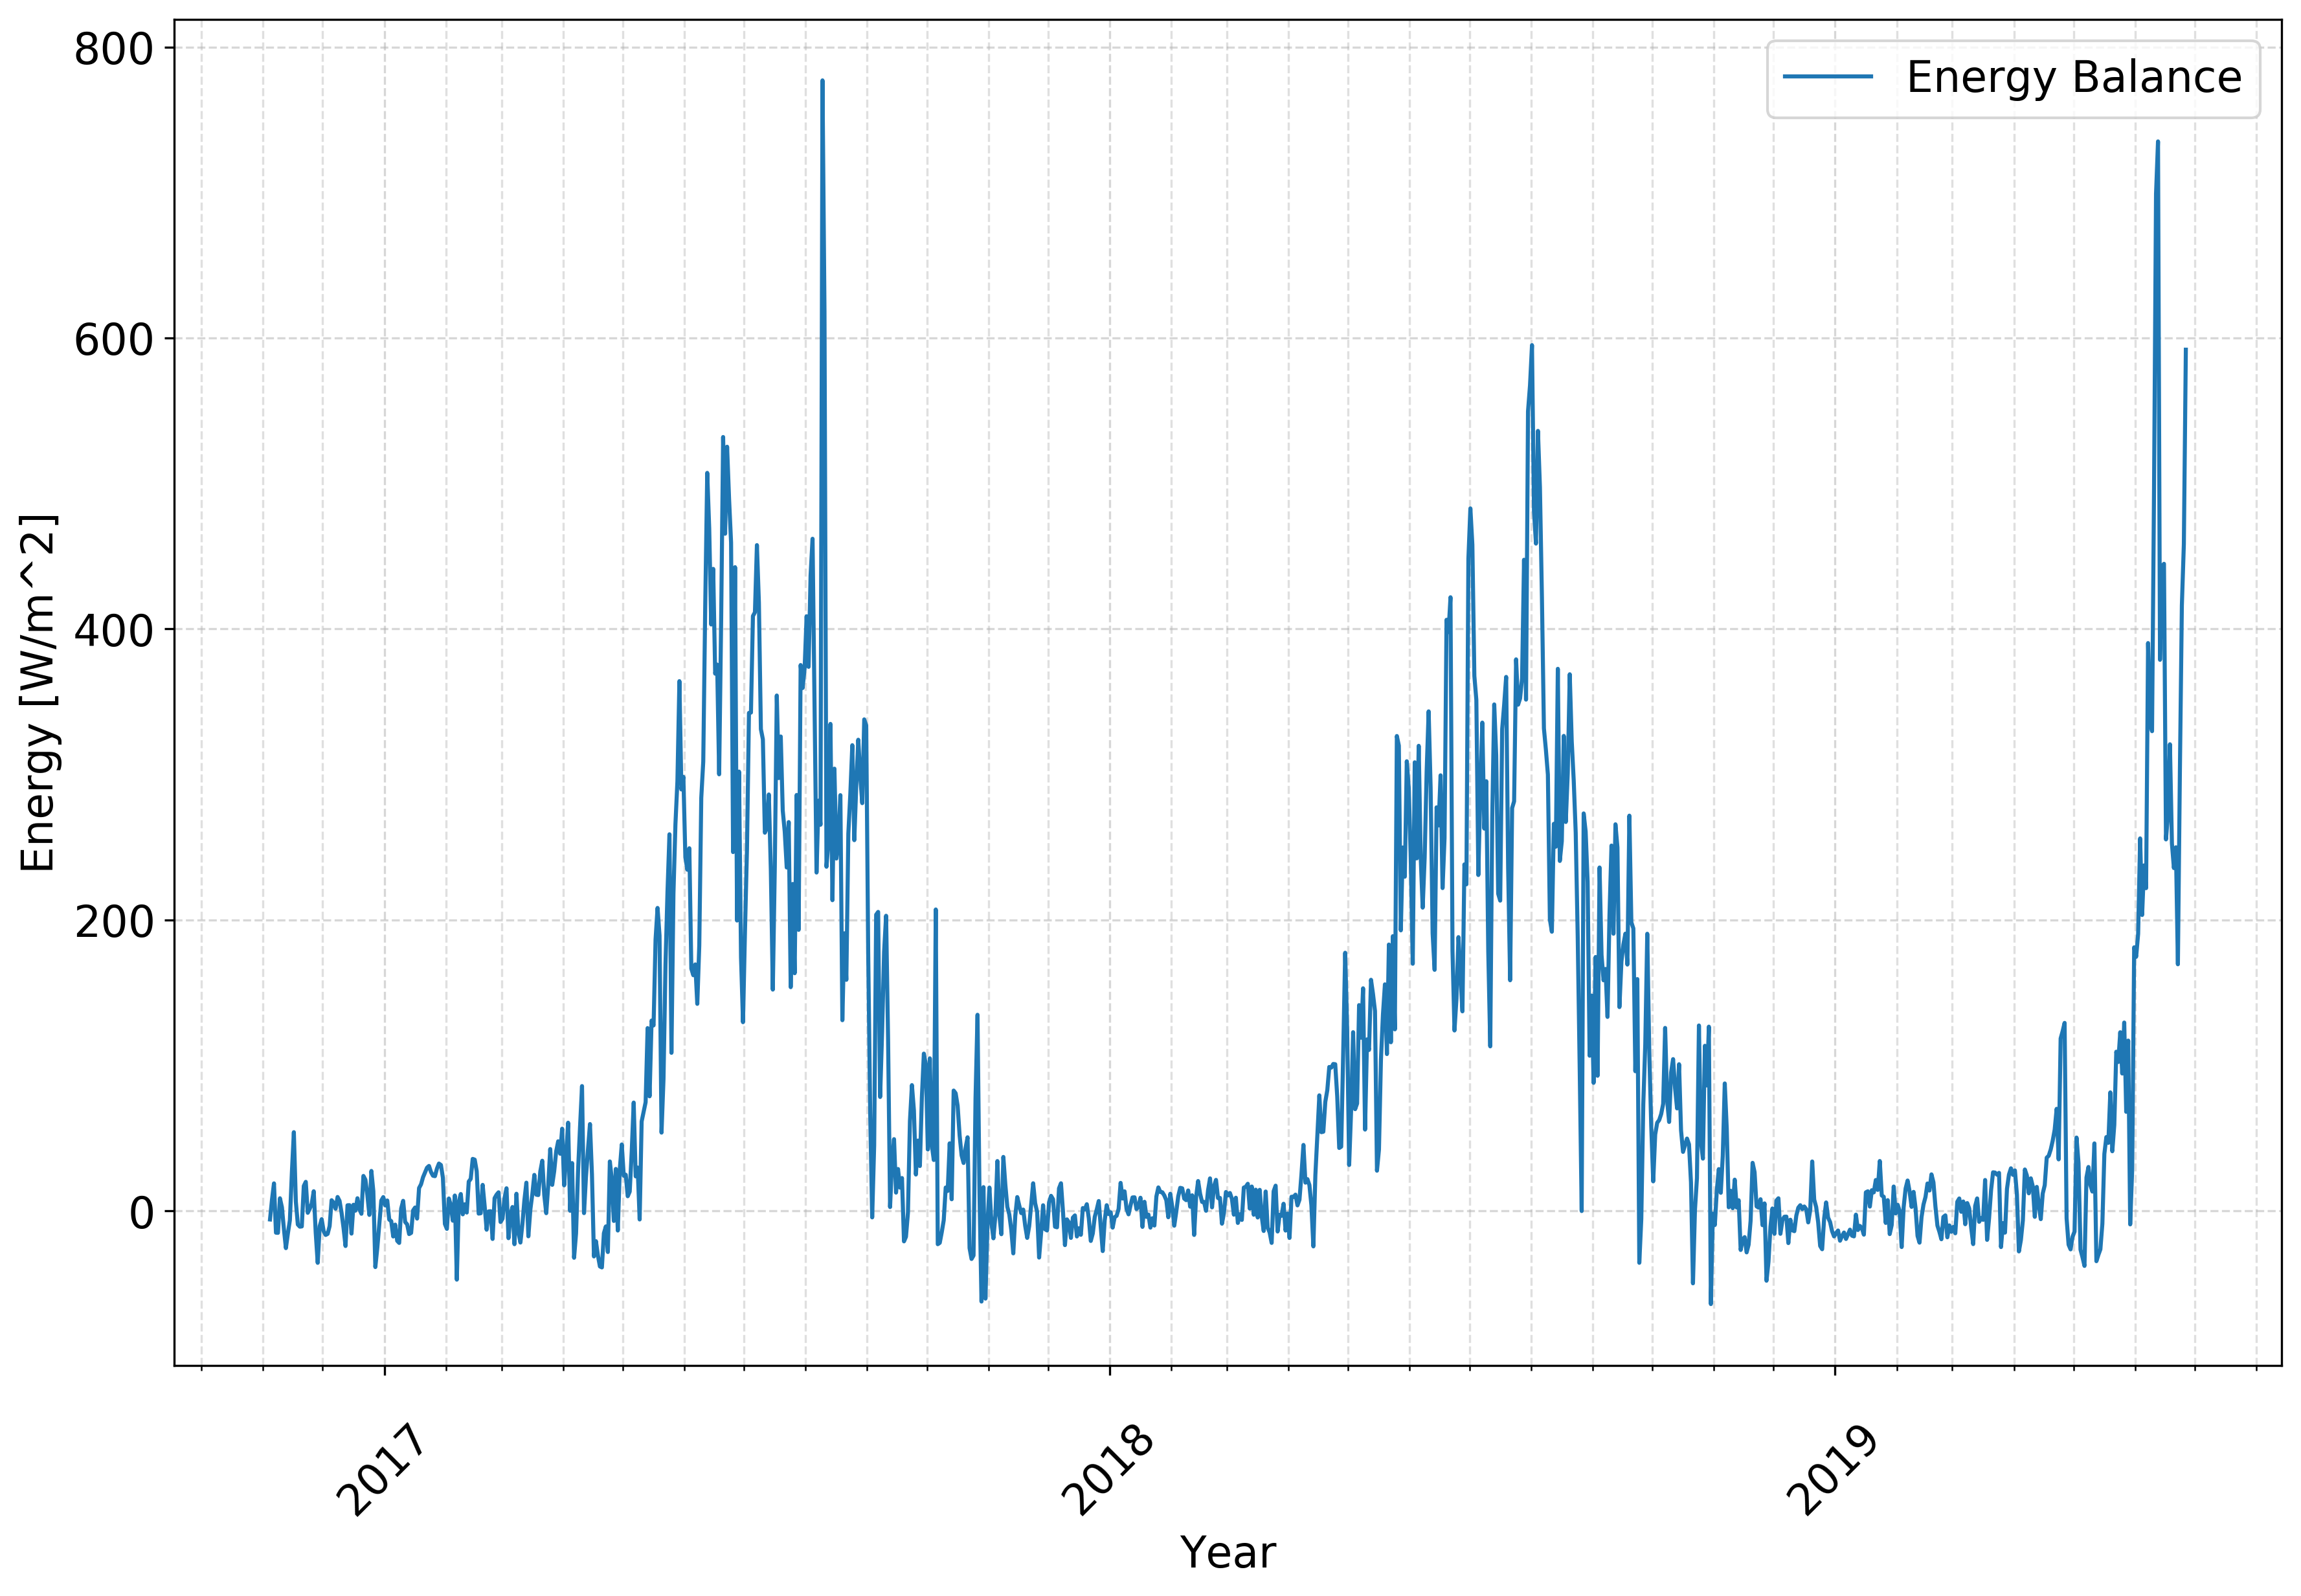
\includegraphics[width=\resultplotsize\textwidth]{../Software/plots/Total_energy_balance_summed.png}
\caption[Energiebilanz, Ablationsgebiet Pasterze im Zeitraum November 2016 bis Juni 2019, Tagesmittel]{Energiebilanz, Ablationsgebiet Pasterze im Zeitraum November 2016 bis Juni 2019, Tagesmittel (Quelle: eigene Darstellung)}
\label{Energiebilanz gesamter Messzeitraum, Tagesmittel}
\end{figure}

Dies resultiert in einem glatteren Verlauf der Kurve, wobei es im Bereich des Sommers zwischen unterschiedlichen Tages-Werten trotzdem noch Abweichungen von teils 300 $W/m^2$ gibt. Dies lässt sich auf unterschiedliche Wetterlagen zurückführen und könnte gut mit Sonnenstunden pro Tag usw. verglichen werden.\\
Das Aufsummieren der Bilanzen bringt zwei Ausreißer nach oben im August 2017 und im Juni 2019 zum Vorschein. Diese Werte, von mehr als 700 $W/m^2$, sind mit knapp 200 $W/m^2$ Vorsprung die größten Werte im betrachteten Zeitraum. Durch Darstellung von einzelnen Komponenten der Energiebilanz kann erörtert werden, woraus diese Maximalwerte hervorgehen.\\

Abbildung \ref{fig:Nettostrahlung (SW und LW) im gesamten Messzeitraum} zeigt die kombinierten Bestandteile ``Short wave in'', ``Short wave out'', ``Long wave in'' und ``Long wave out'', Abbildung \ref{fig:Sensible und latente Wärme im gesamten Messzeitraum} hingegen nur die sensible und latente Wärme. Die periodische Schwingung ist in der ersteren Abbildung deutlicher ausgeprägt.

\begin{figure}[H]
\centering
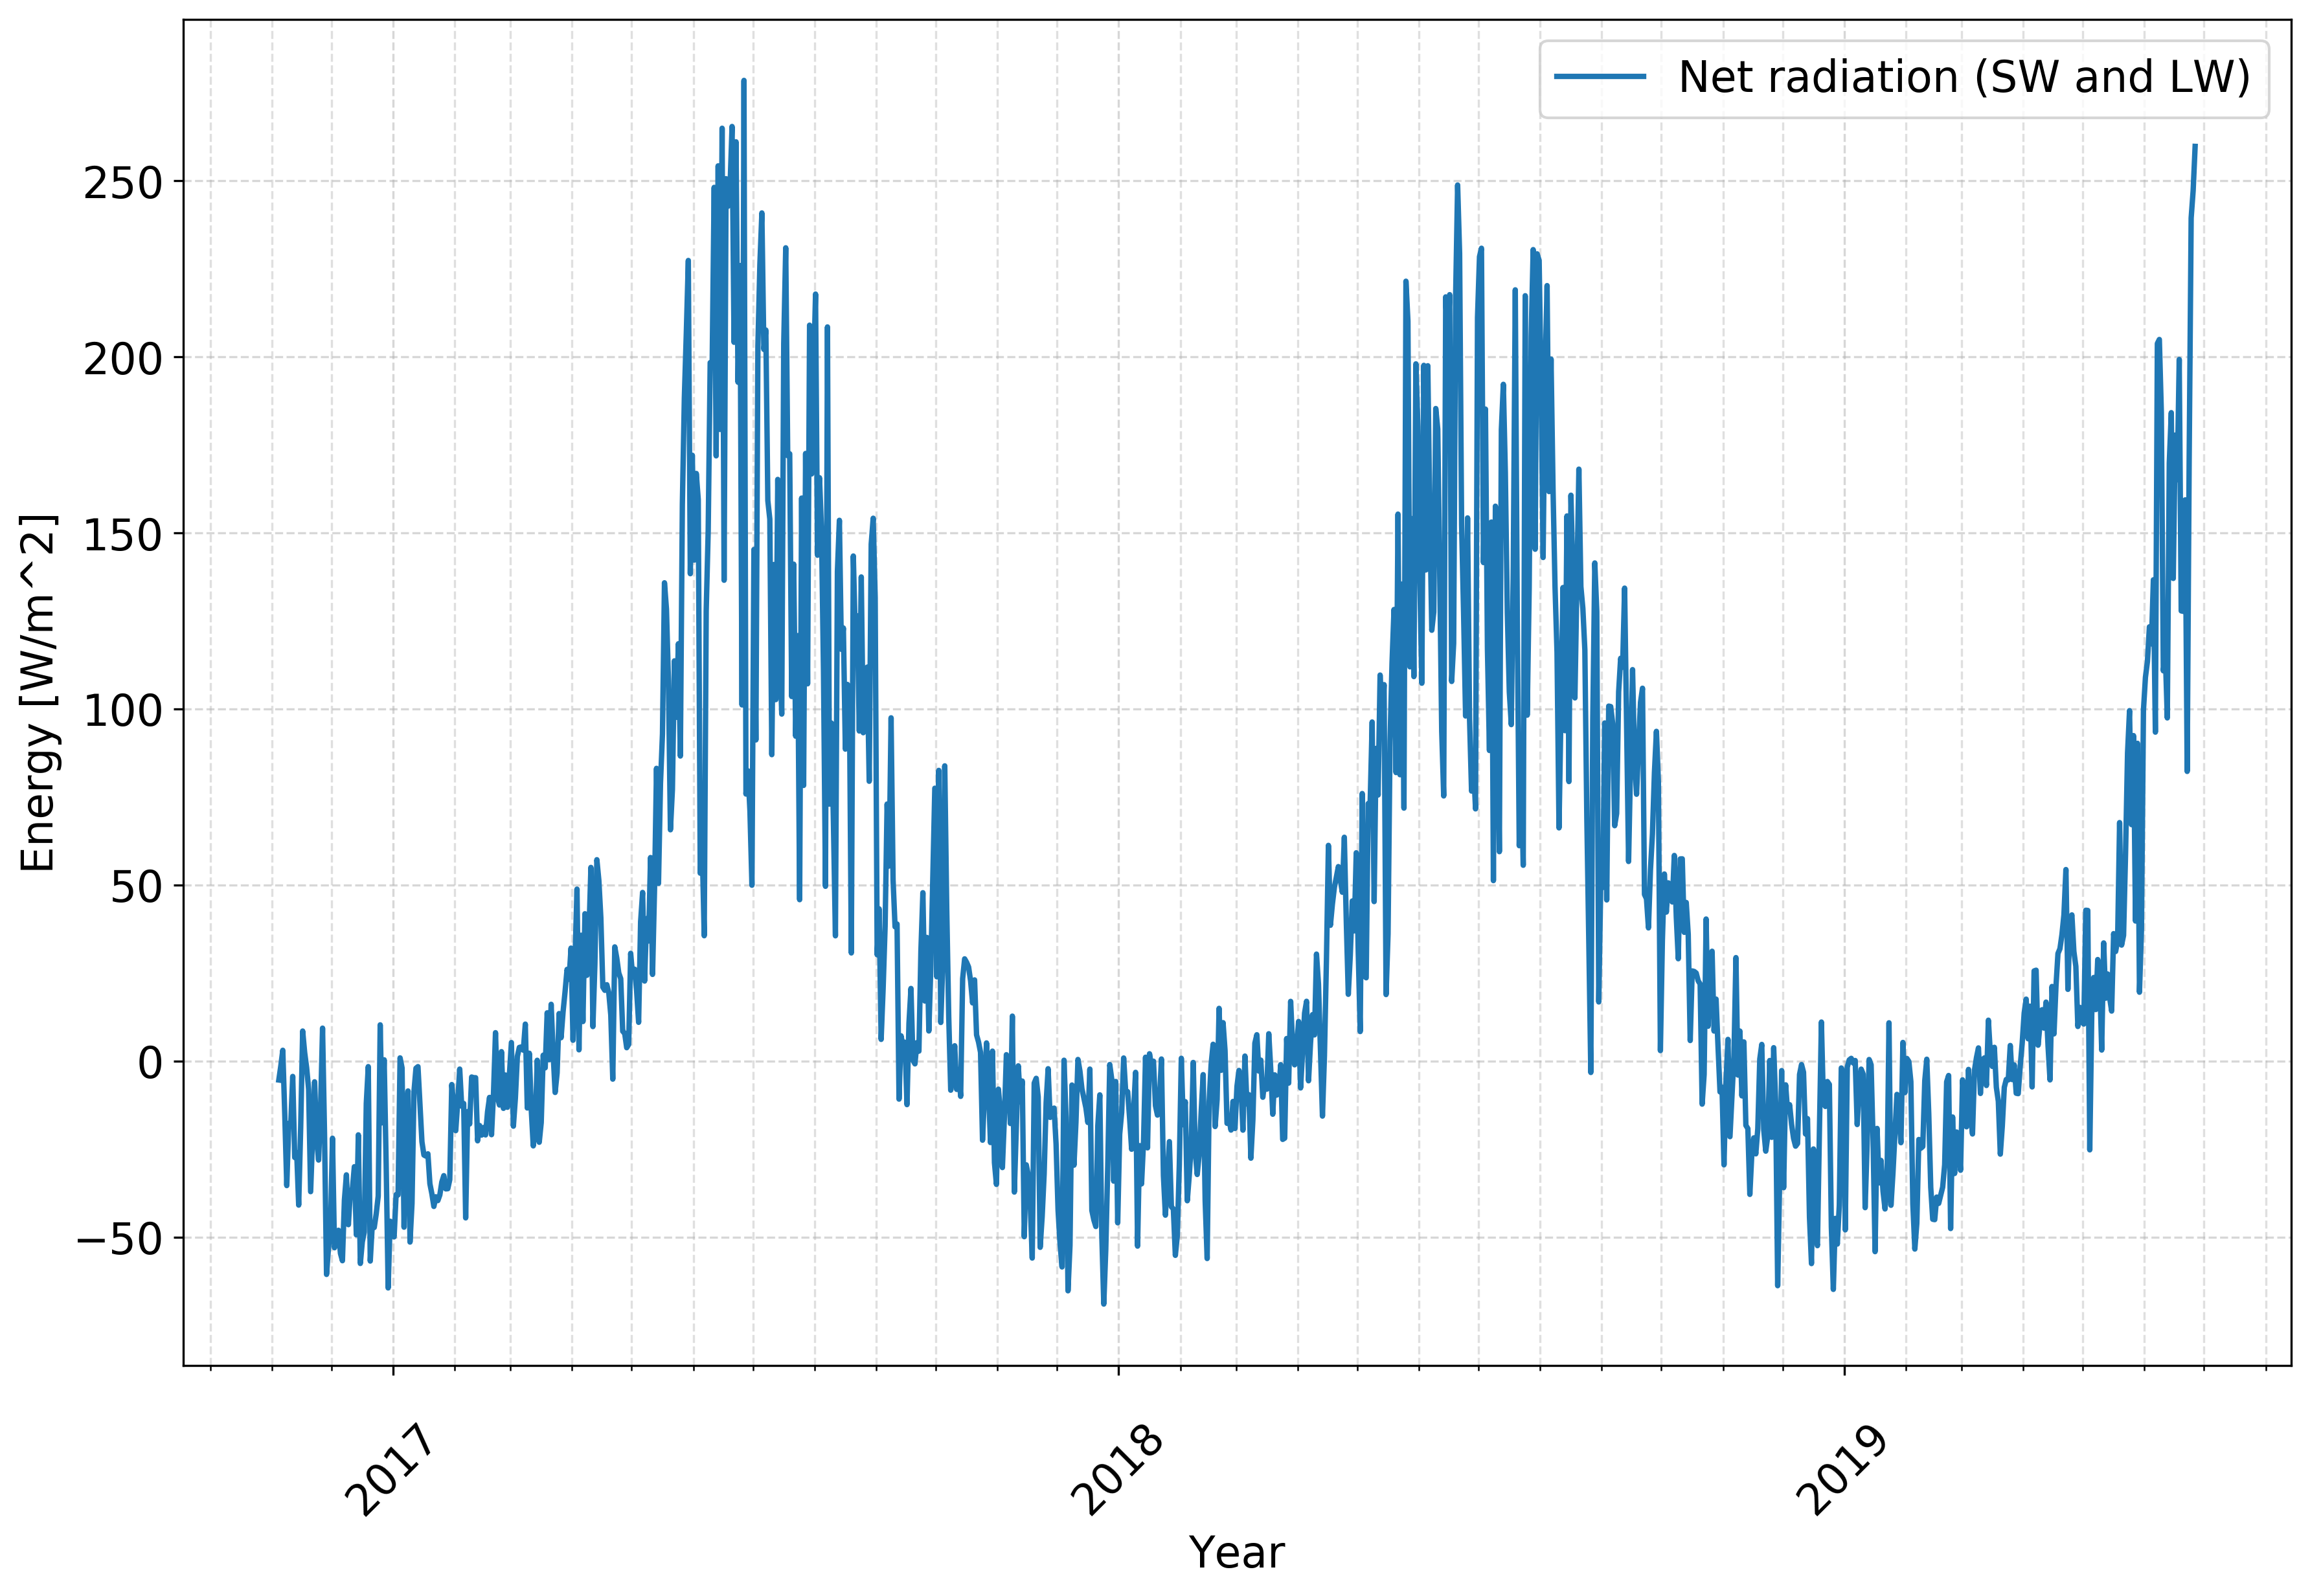
\includegraphics[width=\resultplotsize\textwidth]{../Software/plots/Energy_balance_only_radiation.png}
\caption[Strahlungskomponente, Ablationsgebiet Pasterze im Zeitraum November 2016 bis Juni 2019, Tagesmittel]{Strahlungskomponente, Ablationsgebiet Pasterze im Zeitraum November 2016 bis Juni 2019, Tagesmittel (Quelle: eigene Darstellung)}
\label{fig:Nettostrahlung (SW und LW) im gesamten Messzeitraum}
\end{figure}

\begin{figure}[H]
\centering
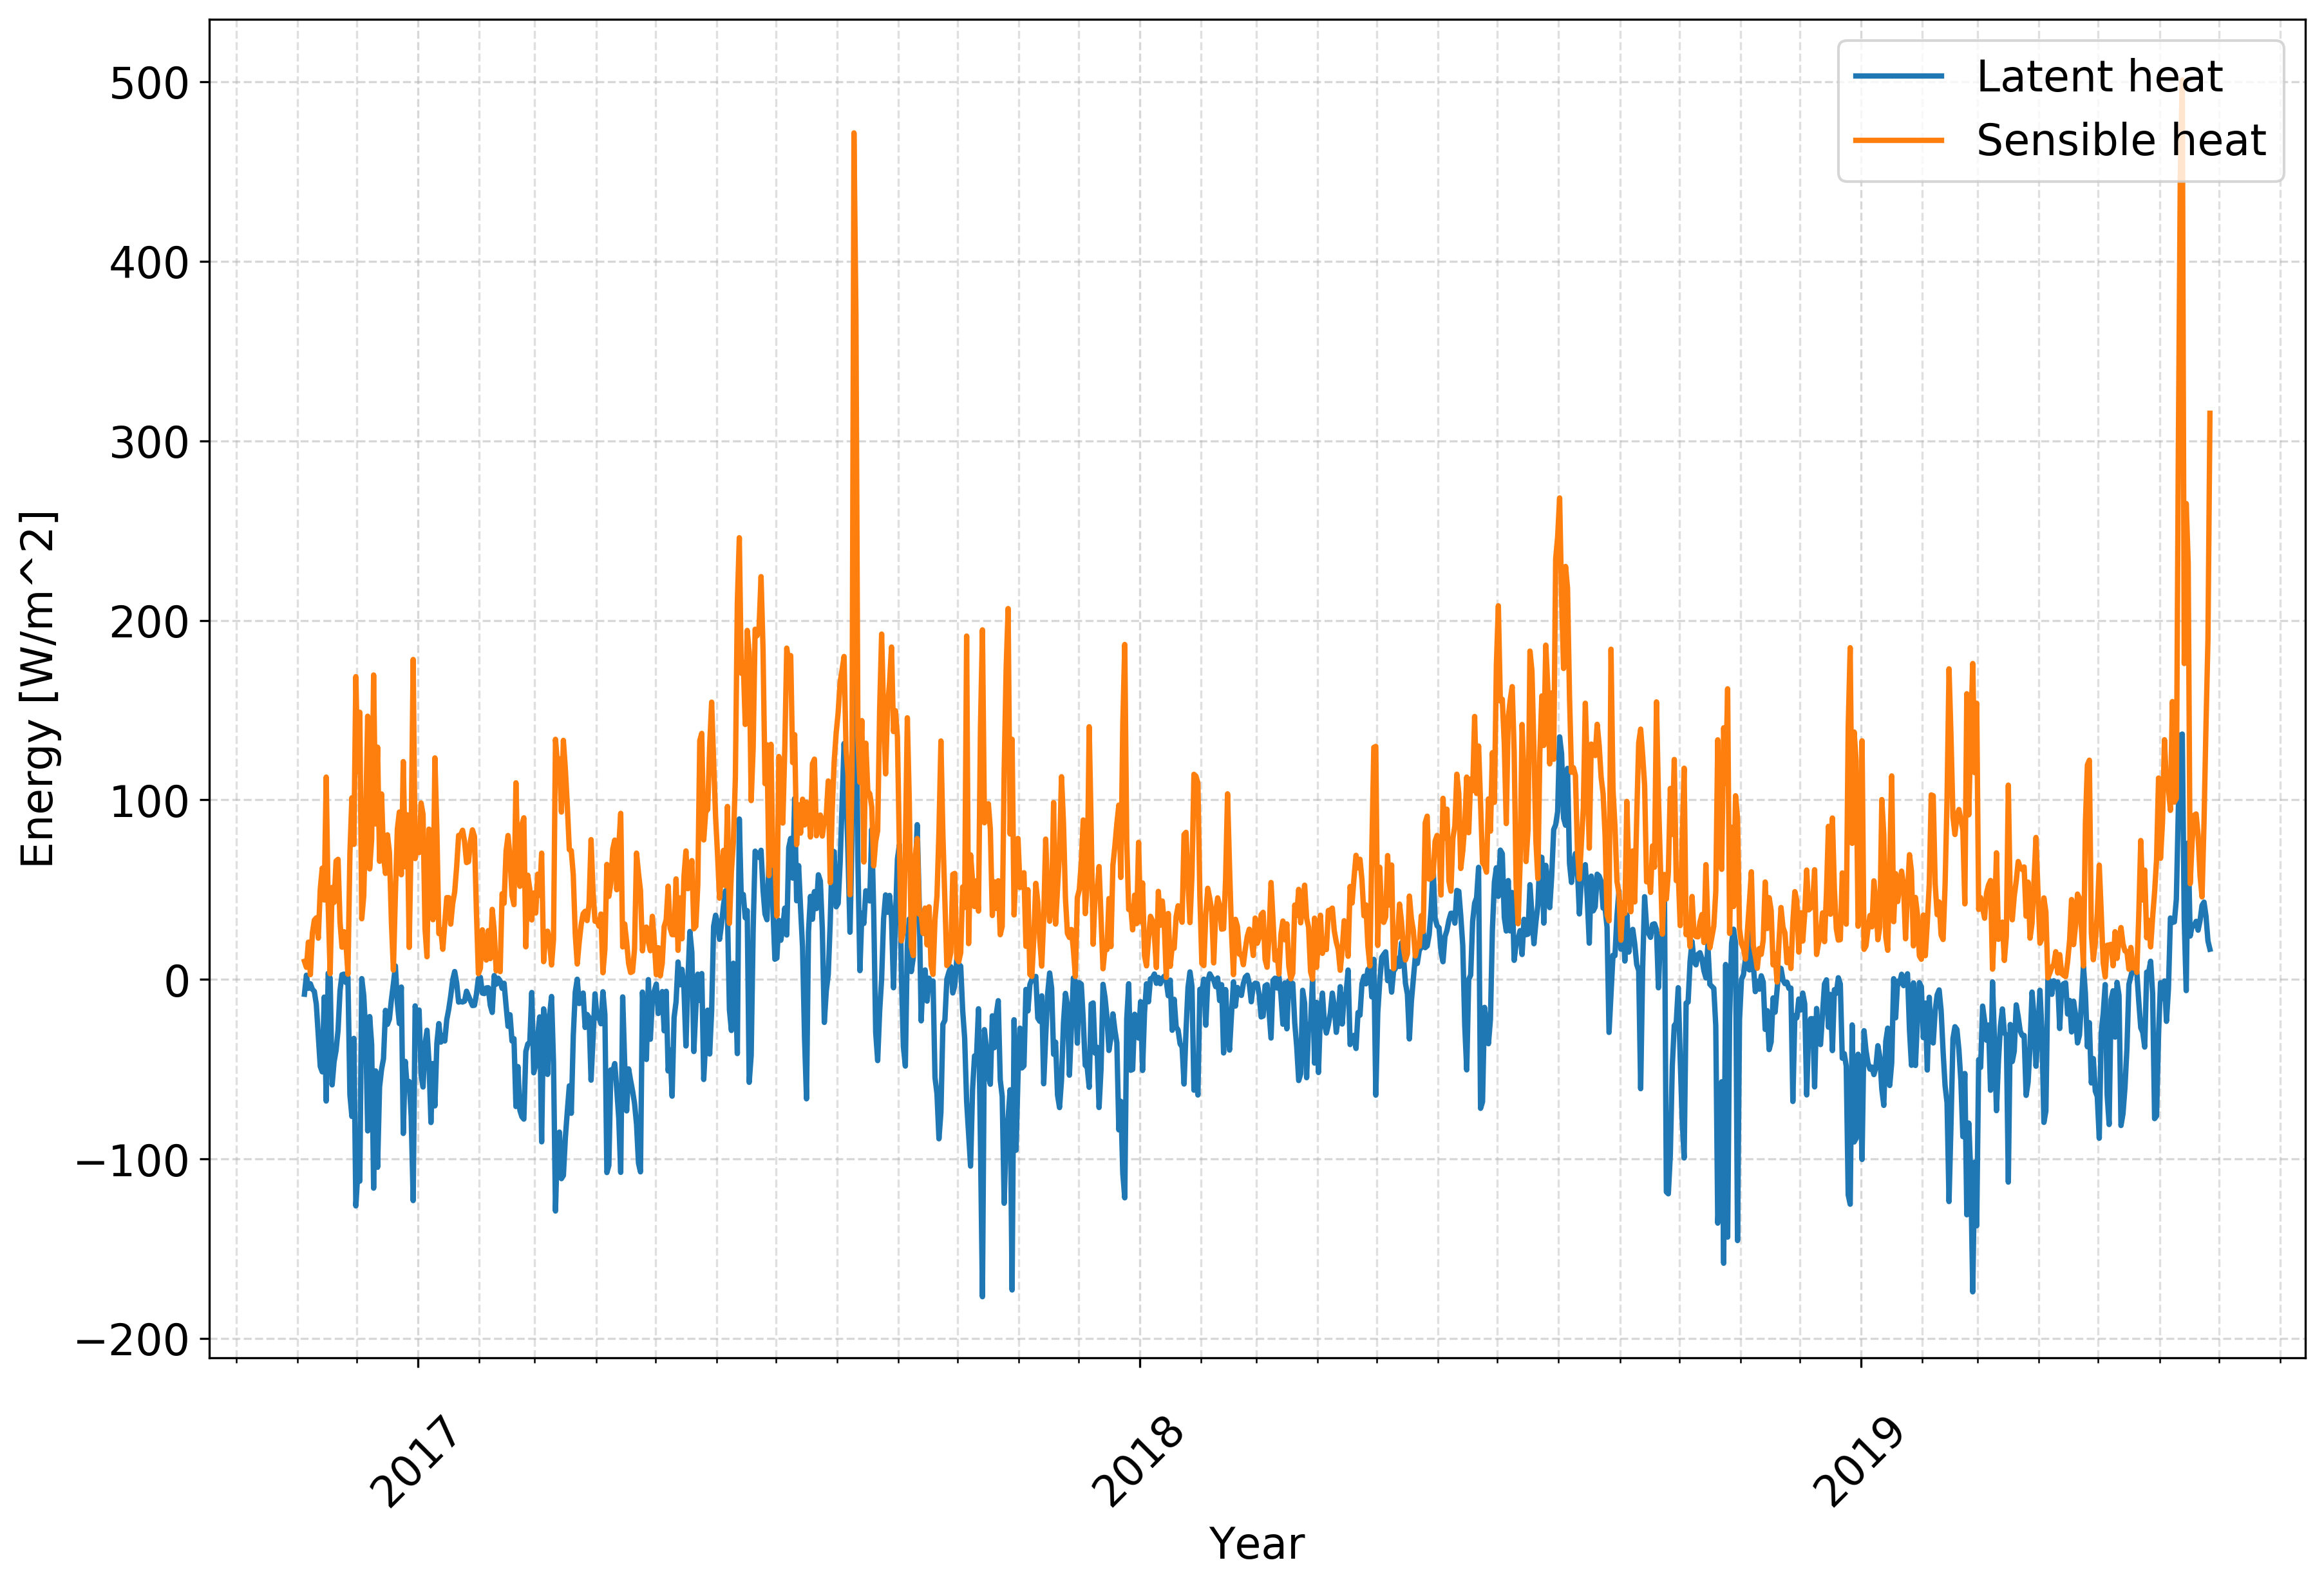
\includegraphics[width=\resultplotsize\textwidth]{../Software/plots/Energy_balance_only_sens_and_latent_heat_accum.png}
\caption[Sensible und latente Wärme, Ablationsgebiet Pasterze im Zeitraum November 2016 bis Juni 2019, Tagesmittel]{Sensible und latente Wärme, Ablationsgebiet Pasterze im Zeitraum November 2016 bis Juni 2019, Tagesmittel (Quelle: eigene Darstellung)}
\label{fig:Sensible und latente Wärme im gesamten Messzeitraum}
\end{figure}

Es stellt sich heraus, dass die genannten, hohen Werte der Energiebilanz bei der sensiblen Wärme auftreten. In der Berechnung der sensiblen Wärme fließen die Messgrößen Luftdruck, Windgeschwindigkeit, Lufttemperatur und Eistemperatur mit ein. Bei genauerer Betrachtung der Messwerte stellt sich heraus, dass alle drei Komponenten zu diesen Zeiten hohe Werte aufweisen. Hohe Temperatur, hoher Luftdruck und gleichzeitig hohe Windgeschwindigkeit resultieren in einem hohen sensiblen Wärmeeintrag. 


\subsection{Ablation $\&$ Schmelzwasser}
In Abbildung \ref{fig:Energiebilanz im gesamten Messzeitraum inklusive Ablationsmessung} wird zusätzlich zur errechneten Energiebilanz die bereinigte Ablation visualisiert. Wie zu erwarten, gibt es immer im Sommer bei hoher Energiebilanz Eisschmelze und im Winter keine Änderung der Ablation. Dies bedeutet allerdings nicht, dass die Masse des Gletschers im Winter stagniert, da in diesem Zeitraum durch Schneefall Akkumulation auftritt, diese aber in der Ablationsmessung nicht sichtbar ist. Zu beobachten ist, dass die Energiebilanz schon vor dem eigentlichen Beginn der Schmelze erhöht ist. Grund dafür ist, dass zuerst der liegende Schnee noch weggeschmolzen werden muss und erst dann die positive Energiebilanz Eisschmelze verursacht.


\begin{figure}[H]
\centering
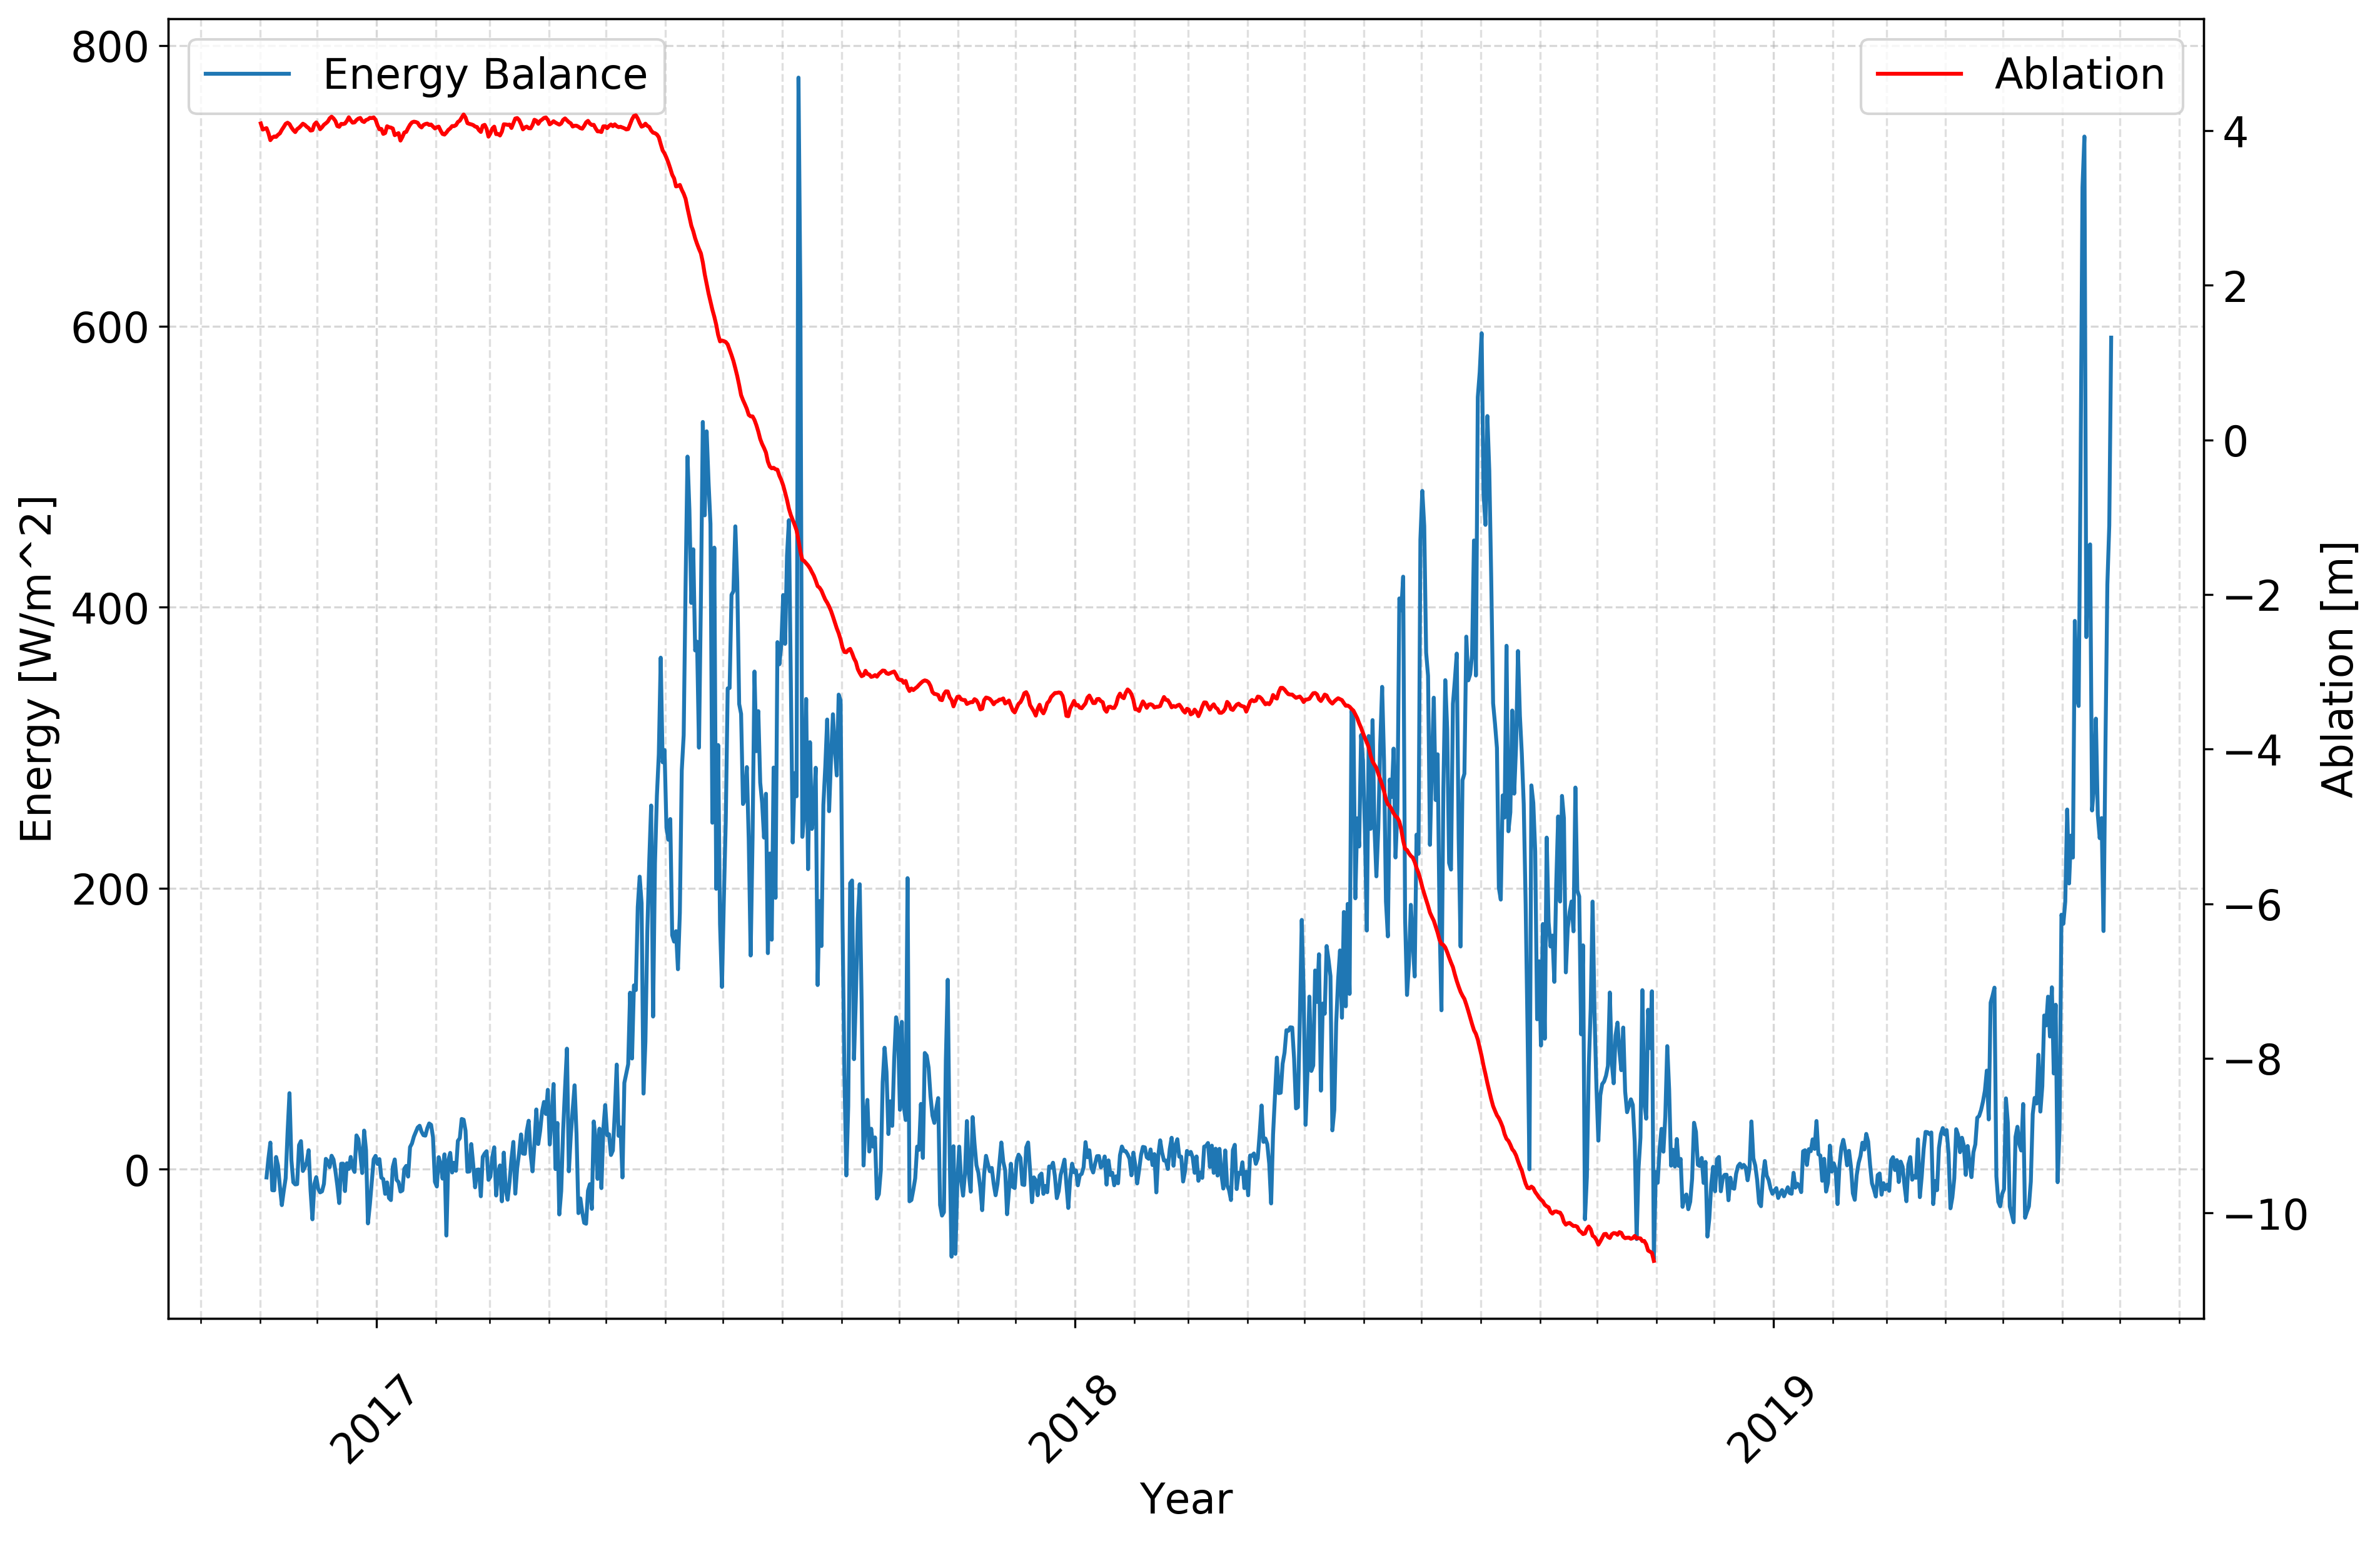
\includegraphics[width=\resultplotsize\textwidth]{../Software/plots/Total_energy_balance_summed_with_ablation.png}
\caption[Energiebilanz inklusive Ablationsmessung, Ablationsgebiet Pasterze im Zeitraum November 2016 bis Juni 2019, Tagesmittel]{Energiebilanz inklusive Ablationsmessung, Ablationsgebiet Pasterze im Zeitraum November 2016 bis Juni 2019, Tagesmittel (Quelle: eigene Darstellung)}
\label{fig:Energiebilanz im gesamten Messzeitraum inklusive Ablationsmessung}
\end{figure}


Folgende Abbildung zeigt die Energiebilanz im gesamten Messzeitraum, wobei zusätzlich das durch die Ablationsmessung errechnete und das modellierte Schmelzwasser aus der Energiebilanz dargestellt wird. Wie bereits in der Methodik (Kapitel \ref{Section Berechnung Schmelzwasser}) erwähnt, wird für die Modellierung nur der Zeitraum zwischen 1. Juni und 1. September pro Jahr verwendet, da zu dieser Zeit der Eislayer als isotherm mit 0 Grad angenommen werden kann, was die Modellierung erleichtert.  

% dass auch im Sommer evtl. Schnellfall auftreten kann und somit die Eisdickenabnahme kurzeitig komplett stoppt. Leider gibt es keine Niederschlagsmessungen, ansonsten könnten diese zusammen mit der Temperatur analysiert werden um so eventuelle    .. sollte nicht der Fall sein





\begin{figure}[H]
\centering
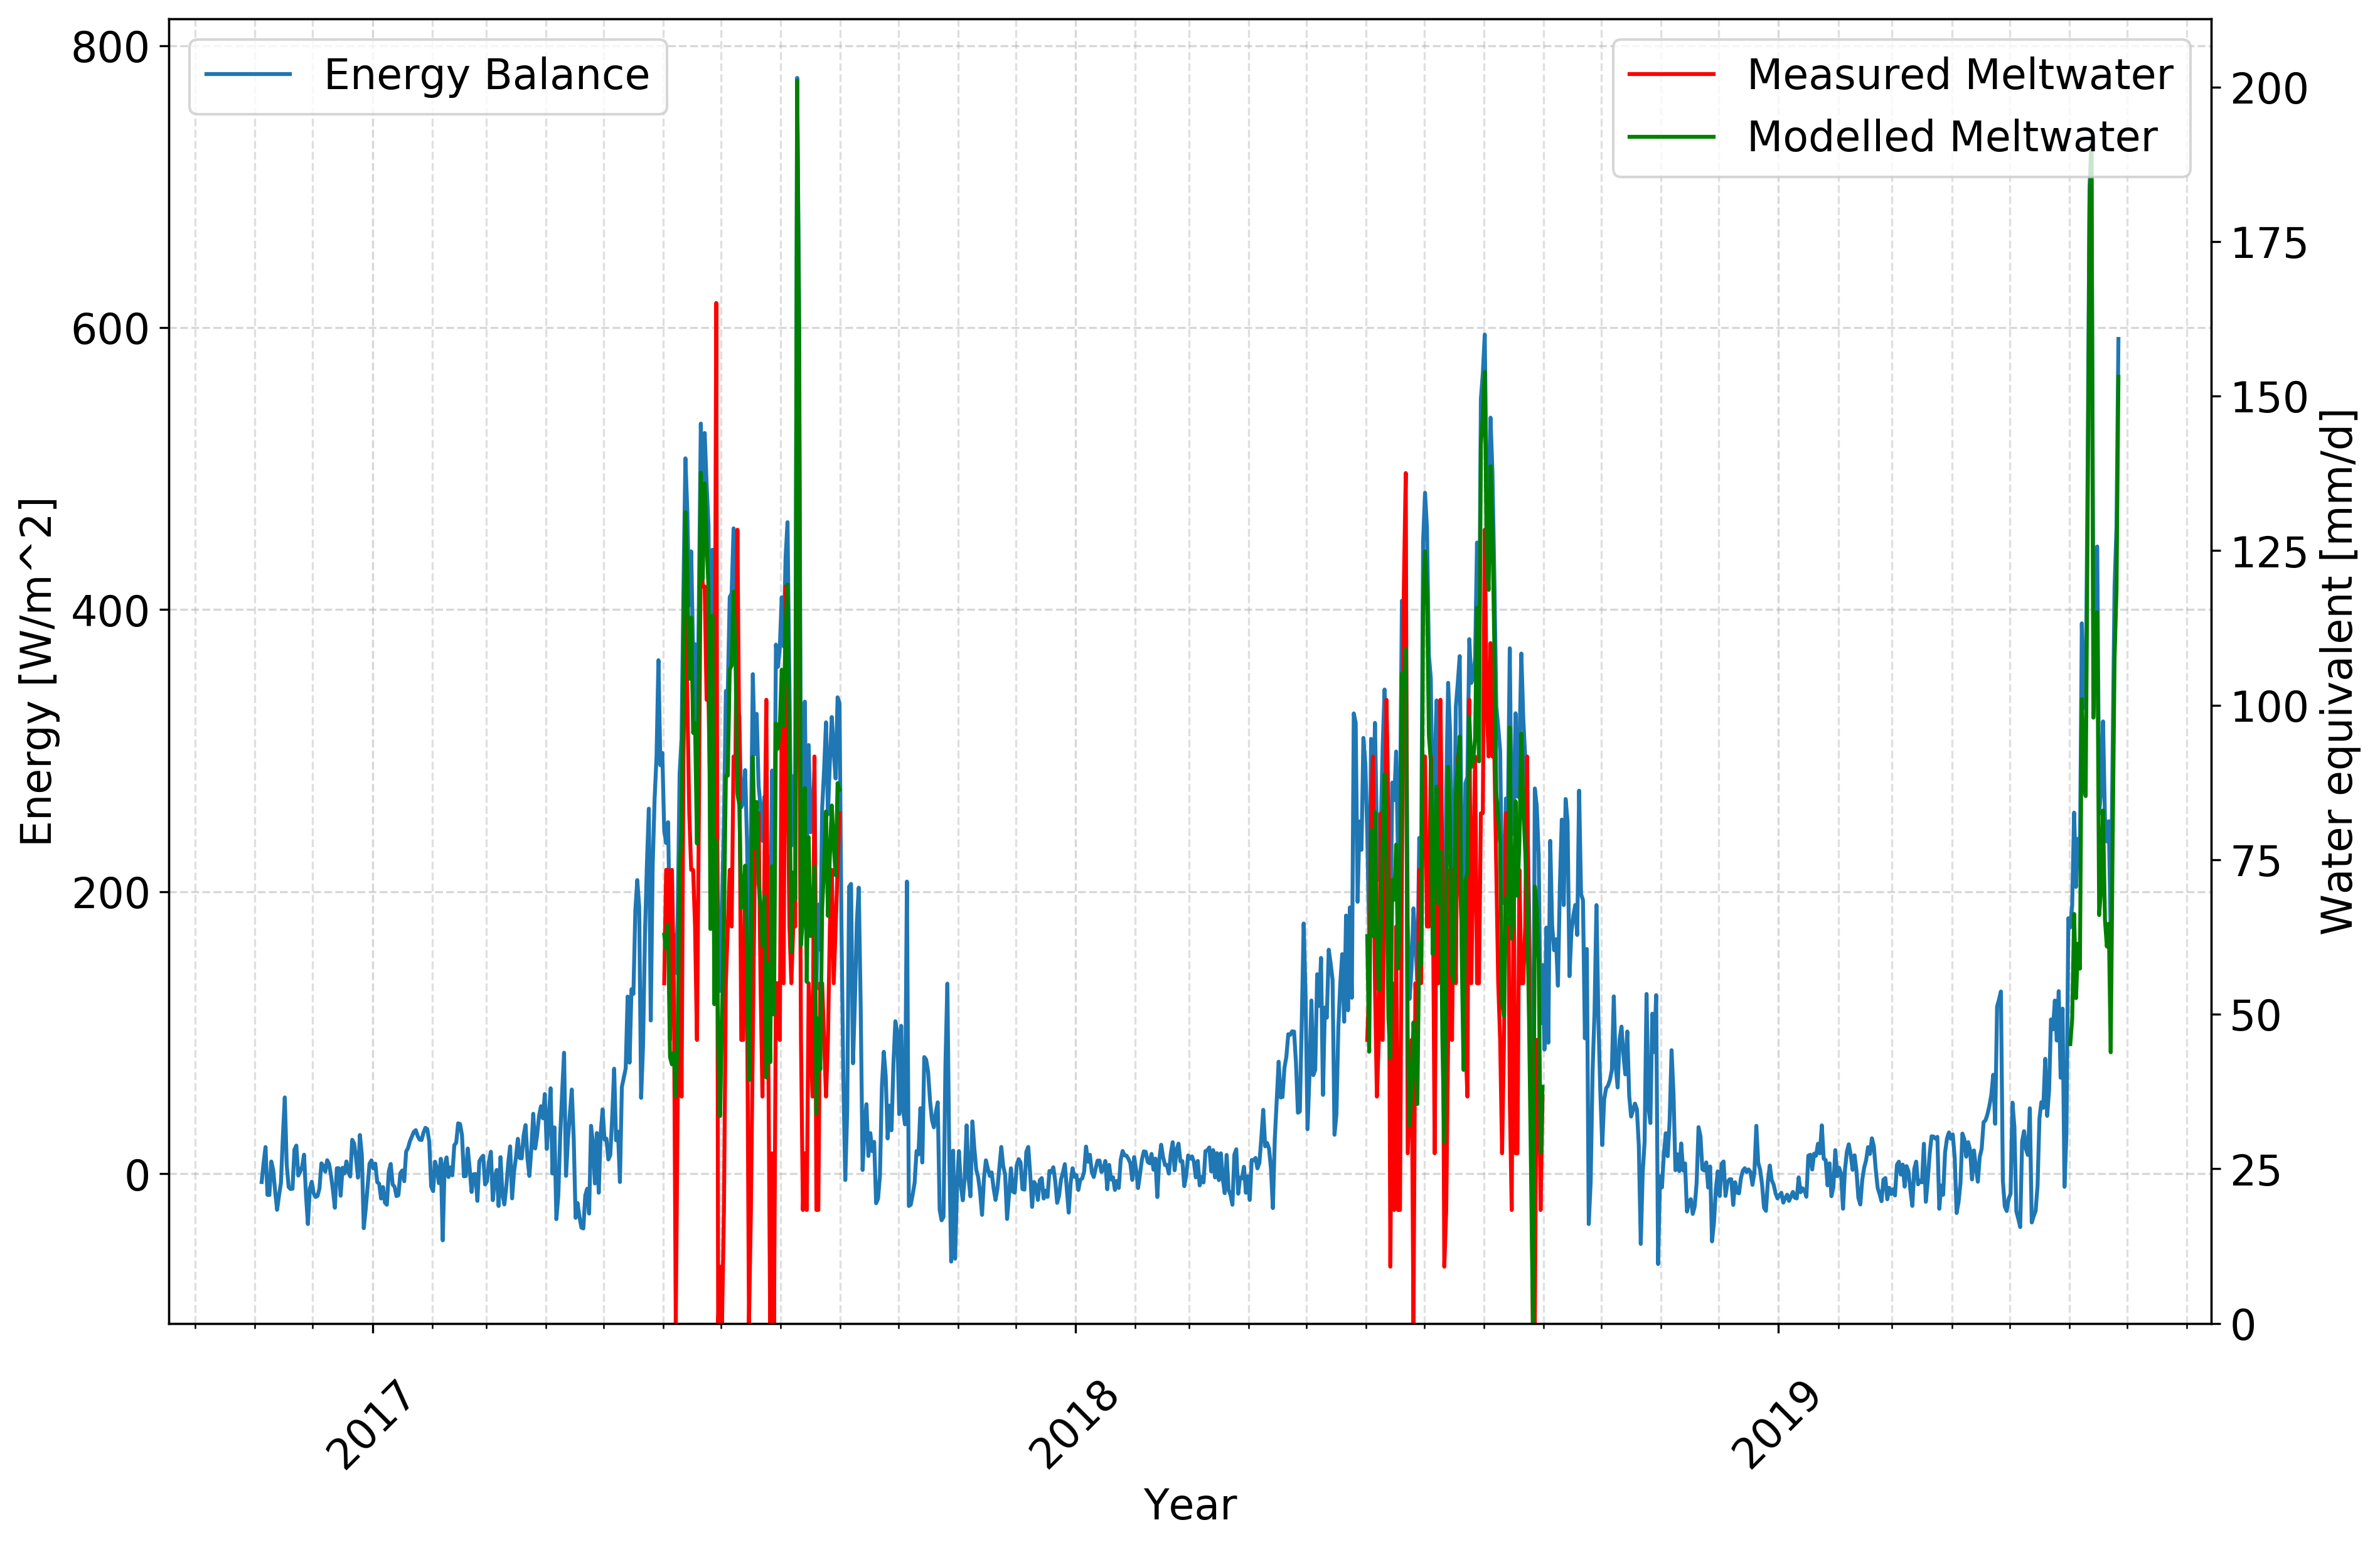
\includegraphics[width=\resultplotsize\textwidth]{../Software/plots/Total_energy_balance_summed_with_water_equivalent.png}
\caption[Energiebilanz inklusive gemessenem und modellierten Schmelzwasser, Ablationsgebiet Pasterze im Zeitraum November 2016 bis Juni 2019, Tagesmittel]{Energiebilanz inklusive gemessenem und modellierten Schmelzwasser, Ablationsgebiet Pasterze im Zeitraum November 2016 bis Juni 2019, Tagesmittel (Quelle: eigene Darstellung)}
\label{fig:Energiebilanz im gesamten Messzeitraum inklusive gemessenem und modellierten Schmelzwasser}
\end{figure}

Auffallend ist, dass das gemessene Schmelzwasser, abweichend zum modellierten, teilweise deutlich weniger ist und im Jahr 2017 sogar häufig bei 0 [mm/d] liegt. Kein gemessenes Schmelzwasser bedeutet, dass in der Ablationsmessung kein Rückgang der Eisdicke zu erkennen ist. Wird Abbildung \ref{Vergleich gemessenes Schmelzwasser und Temperatur} betrachet, so kann erkannt werden, dass teils trotz Tagesdurchschnittstemperatur über ca. $4^\circ C$ keine Ablation gemessen wird. Ob nun das Modell in diesen Fällen falsch ist, oder ob die Ablationsmessung mit groben Fehlern behaftet ist, könnte anhand von anderen Gletschern und den dazugehörigen Messwerten überprüft werden.

\begin{figure}[H]
\centering
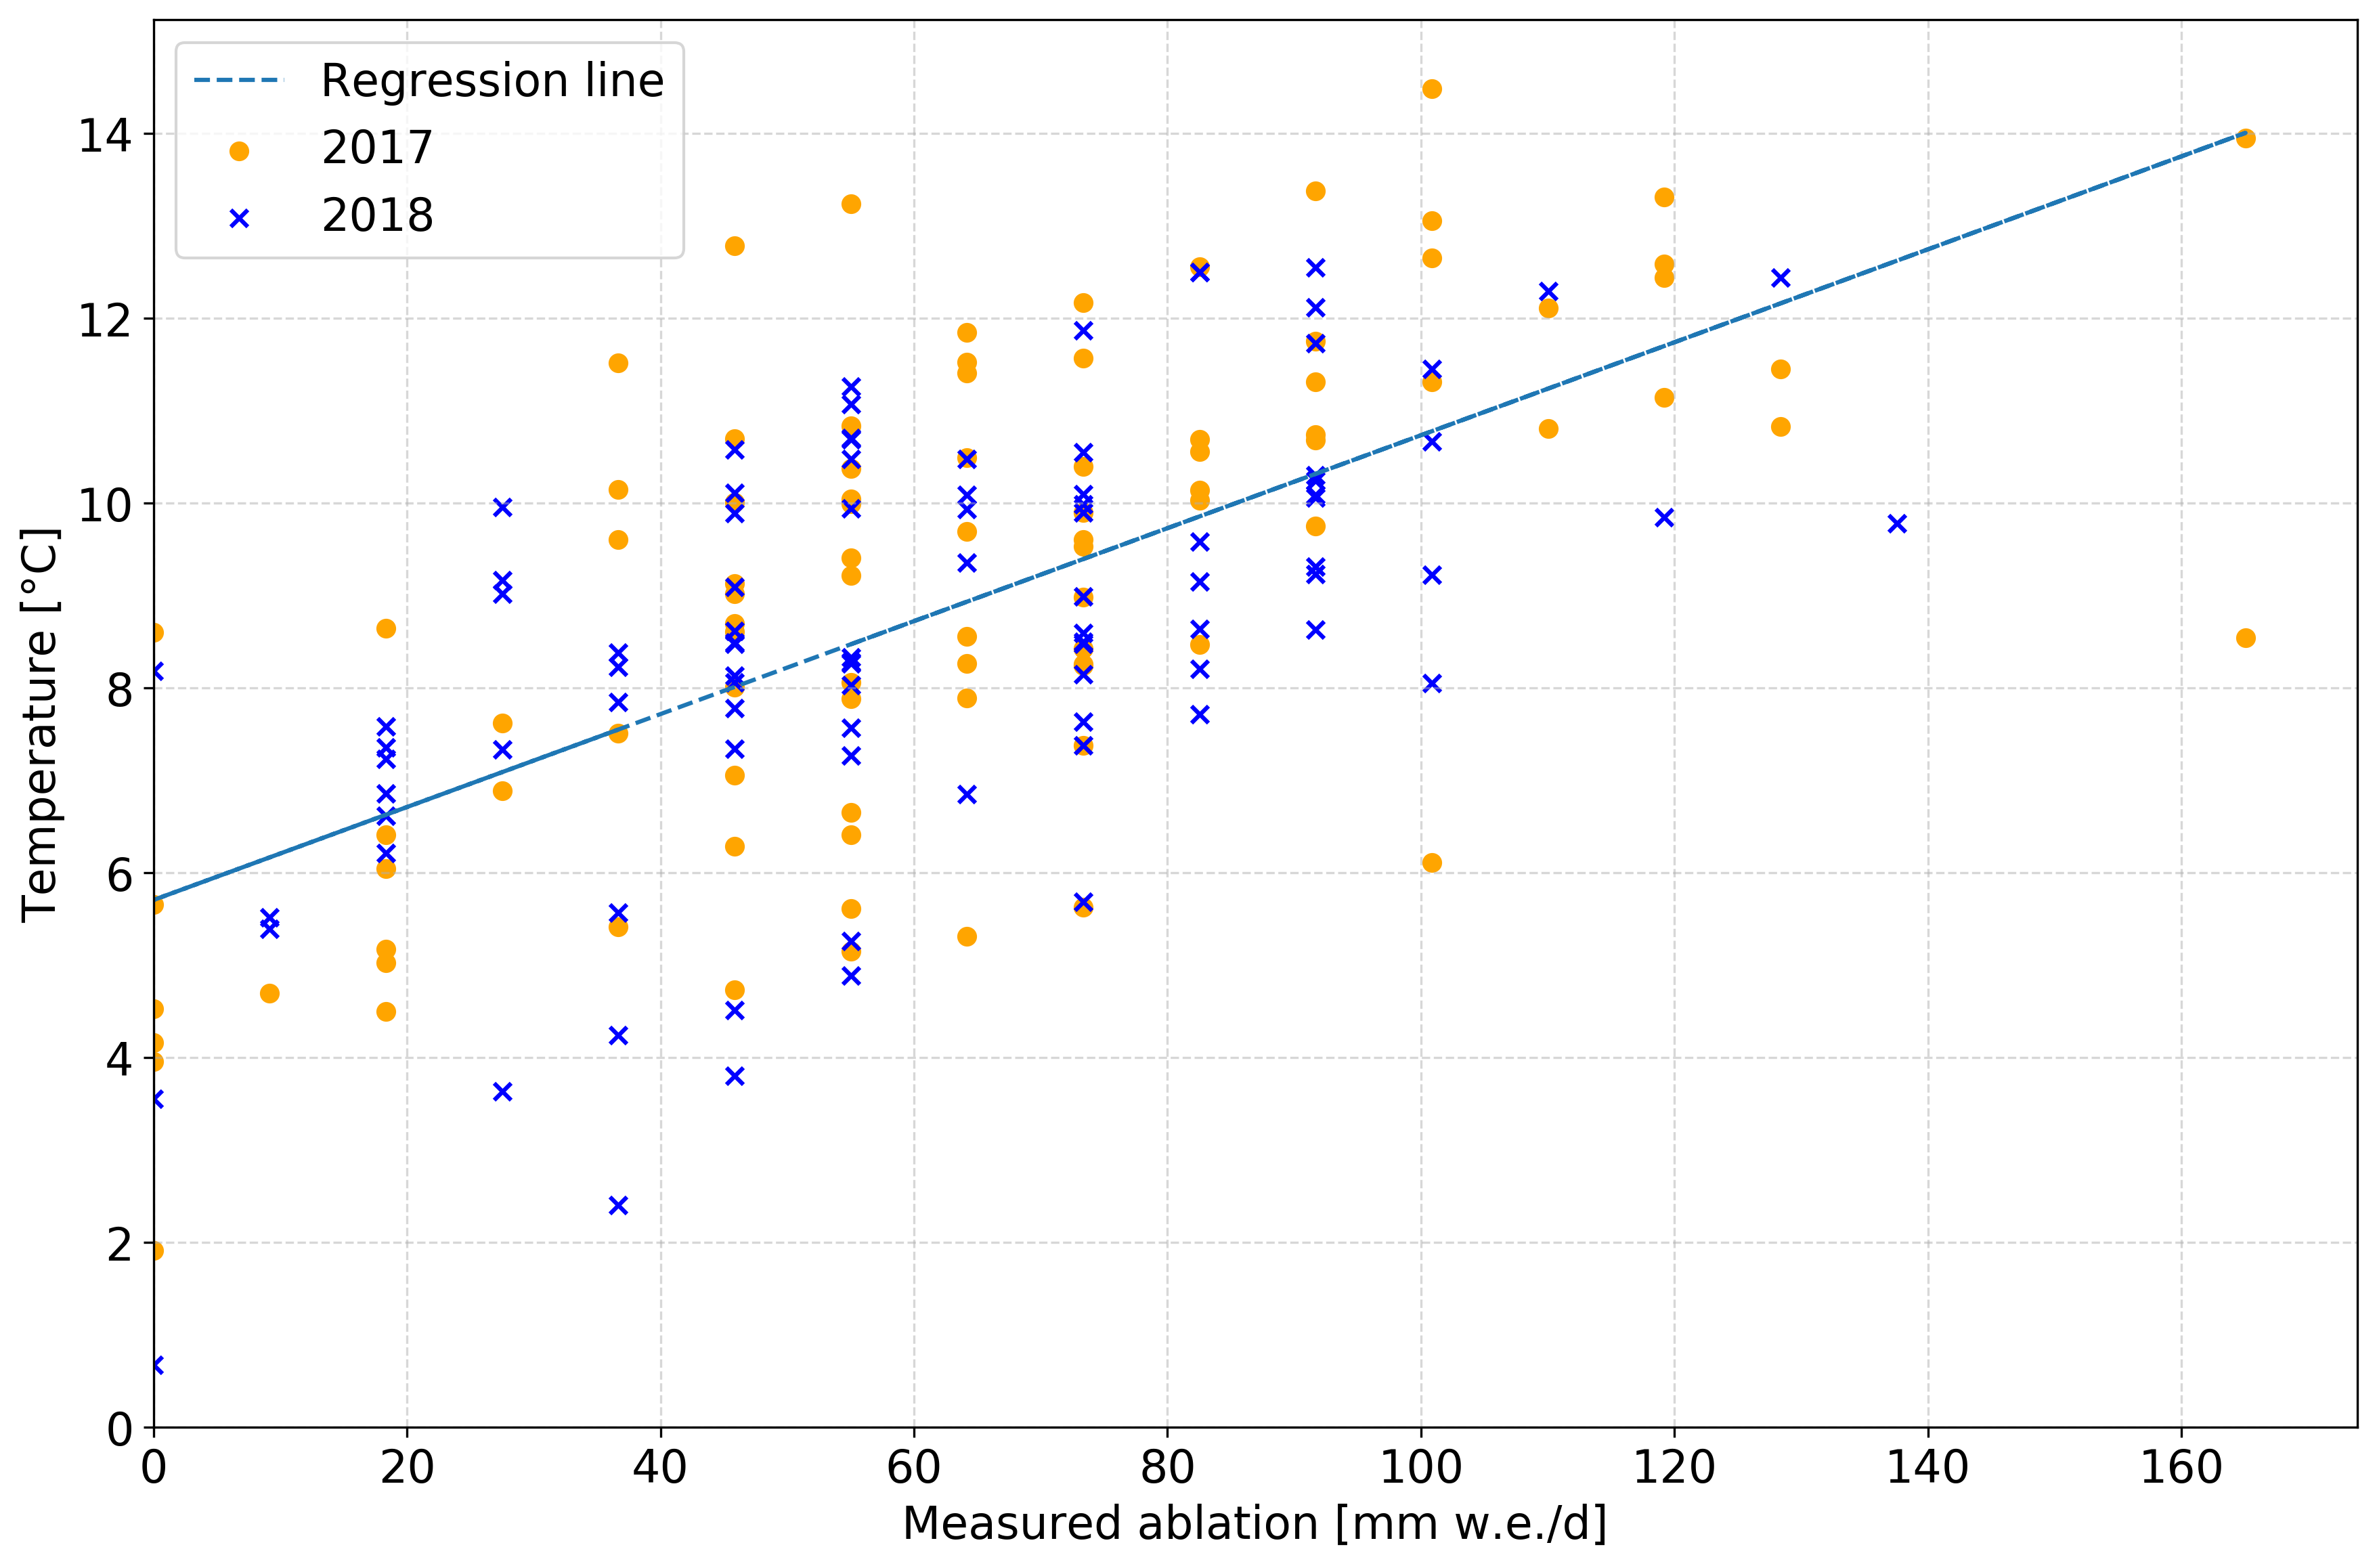
\includegraphics[width=\resultplotsize\textwidth]{../Software/plots/Scatter_measured_water_equivalent_and_temperature.png}
\caption[Vergleich gemessenes Schmelzwasser und Temperaturtagesmittel, Ablationsgebiet Pasterze im Zeitraum 2017 und 2018]{Vergleich gemessenes Schmelzwasser und Temperatur, Ablationsgebiet Pasterze im Zeitraum 2017 und 2018 (Quelle: eigene Darstellung)}
\label{Vergleich gemessenes Schmelzwasser und Temperatur}
\end{figure}

Abbildung \ref{fig:Energiebilanz im Sommer 2017 inklusive der in Wasseräquivalent umgerechneten Ablation und dem modellierten Schmelzwasser} und \ref{Energiebilanz im Sommer 2018 inklusive der in Wasseräquivalent umgerechneten Ablation und dem modellierten Schmelzwasser} zeigen den Zusammenhang in Abbildung \ref{fig:Energiebilanz im gesamten Messzeitraum inklusive gemessenem und modellierten Schmelzwasser} für die zwei Jahre 2017 und 2018 vergrößert auf. Tendenziell wird im Modell insbesondere bei Energiebilanzspitzen eine größere Menge an Schmelzwasser angenommen. Der Verlauf der Kurve vom gemessenen Schmelzwasser an sich wird aber sehr gut von der Kurve des modellierten Schmelzwasser wiedergegeben. In folgender Tabelle wird diese visuelle Interpretation in Form vom Korrelationskoeffizienten nach Pearson in Zahlen ausgedrückt. 


\begin{table}[H]
\centering
\setstretch{1.3} 
\caption{Korrelation zwischen gemessenem und modellierten Schmelzwasser}
\label{tab:Korrelation zwischen gemessenem und modellierten Schmelzwasser}
\begin{tabular}{|l|l|}
\hline
Sommermonate & Korrelation nach Pearson \\ \hline
2017         & 0.72                     \\ \hline
2018         & 0.63                     \\ \hline
\end{tabular}
\end{table}

Ab einer Korrelation von 0.7 wird von einer starken Korrelation gesprochen. Das angenommene Modell repräsentiert also durchaus die Realität.

\begin{figure}[H]
\centering
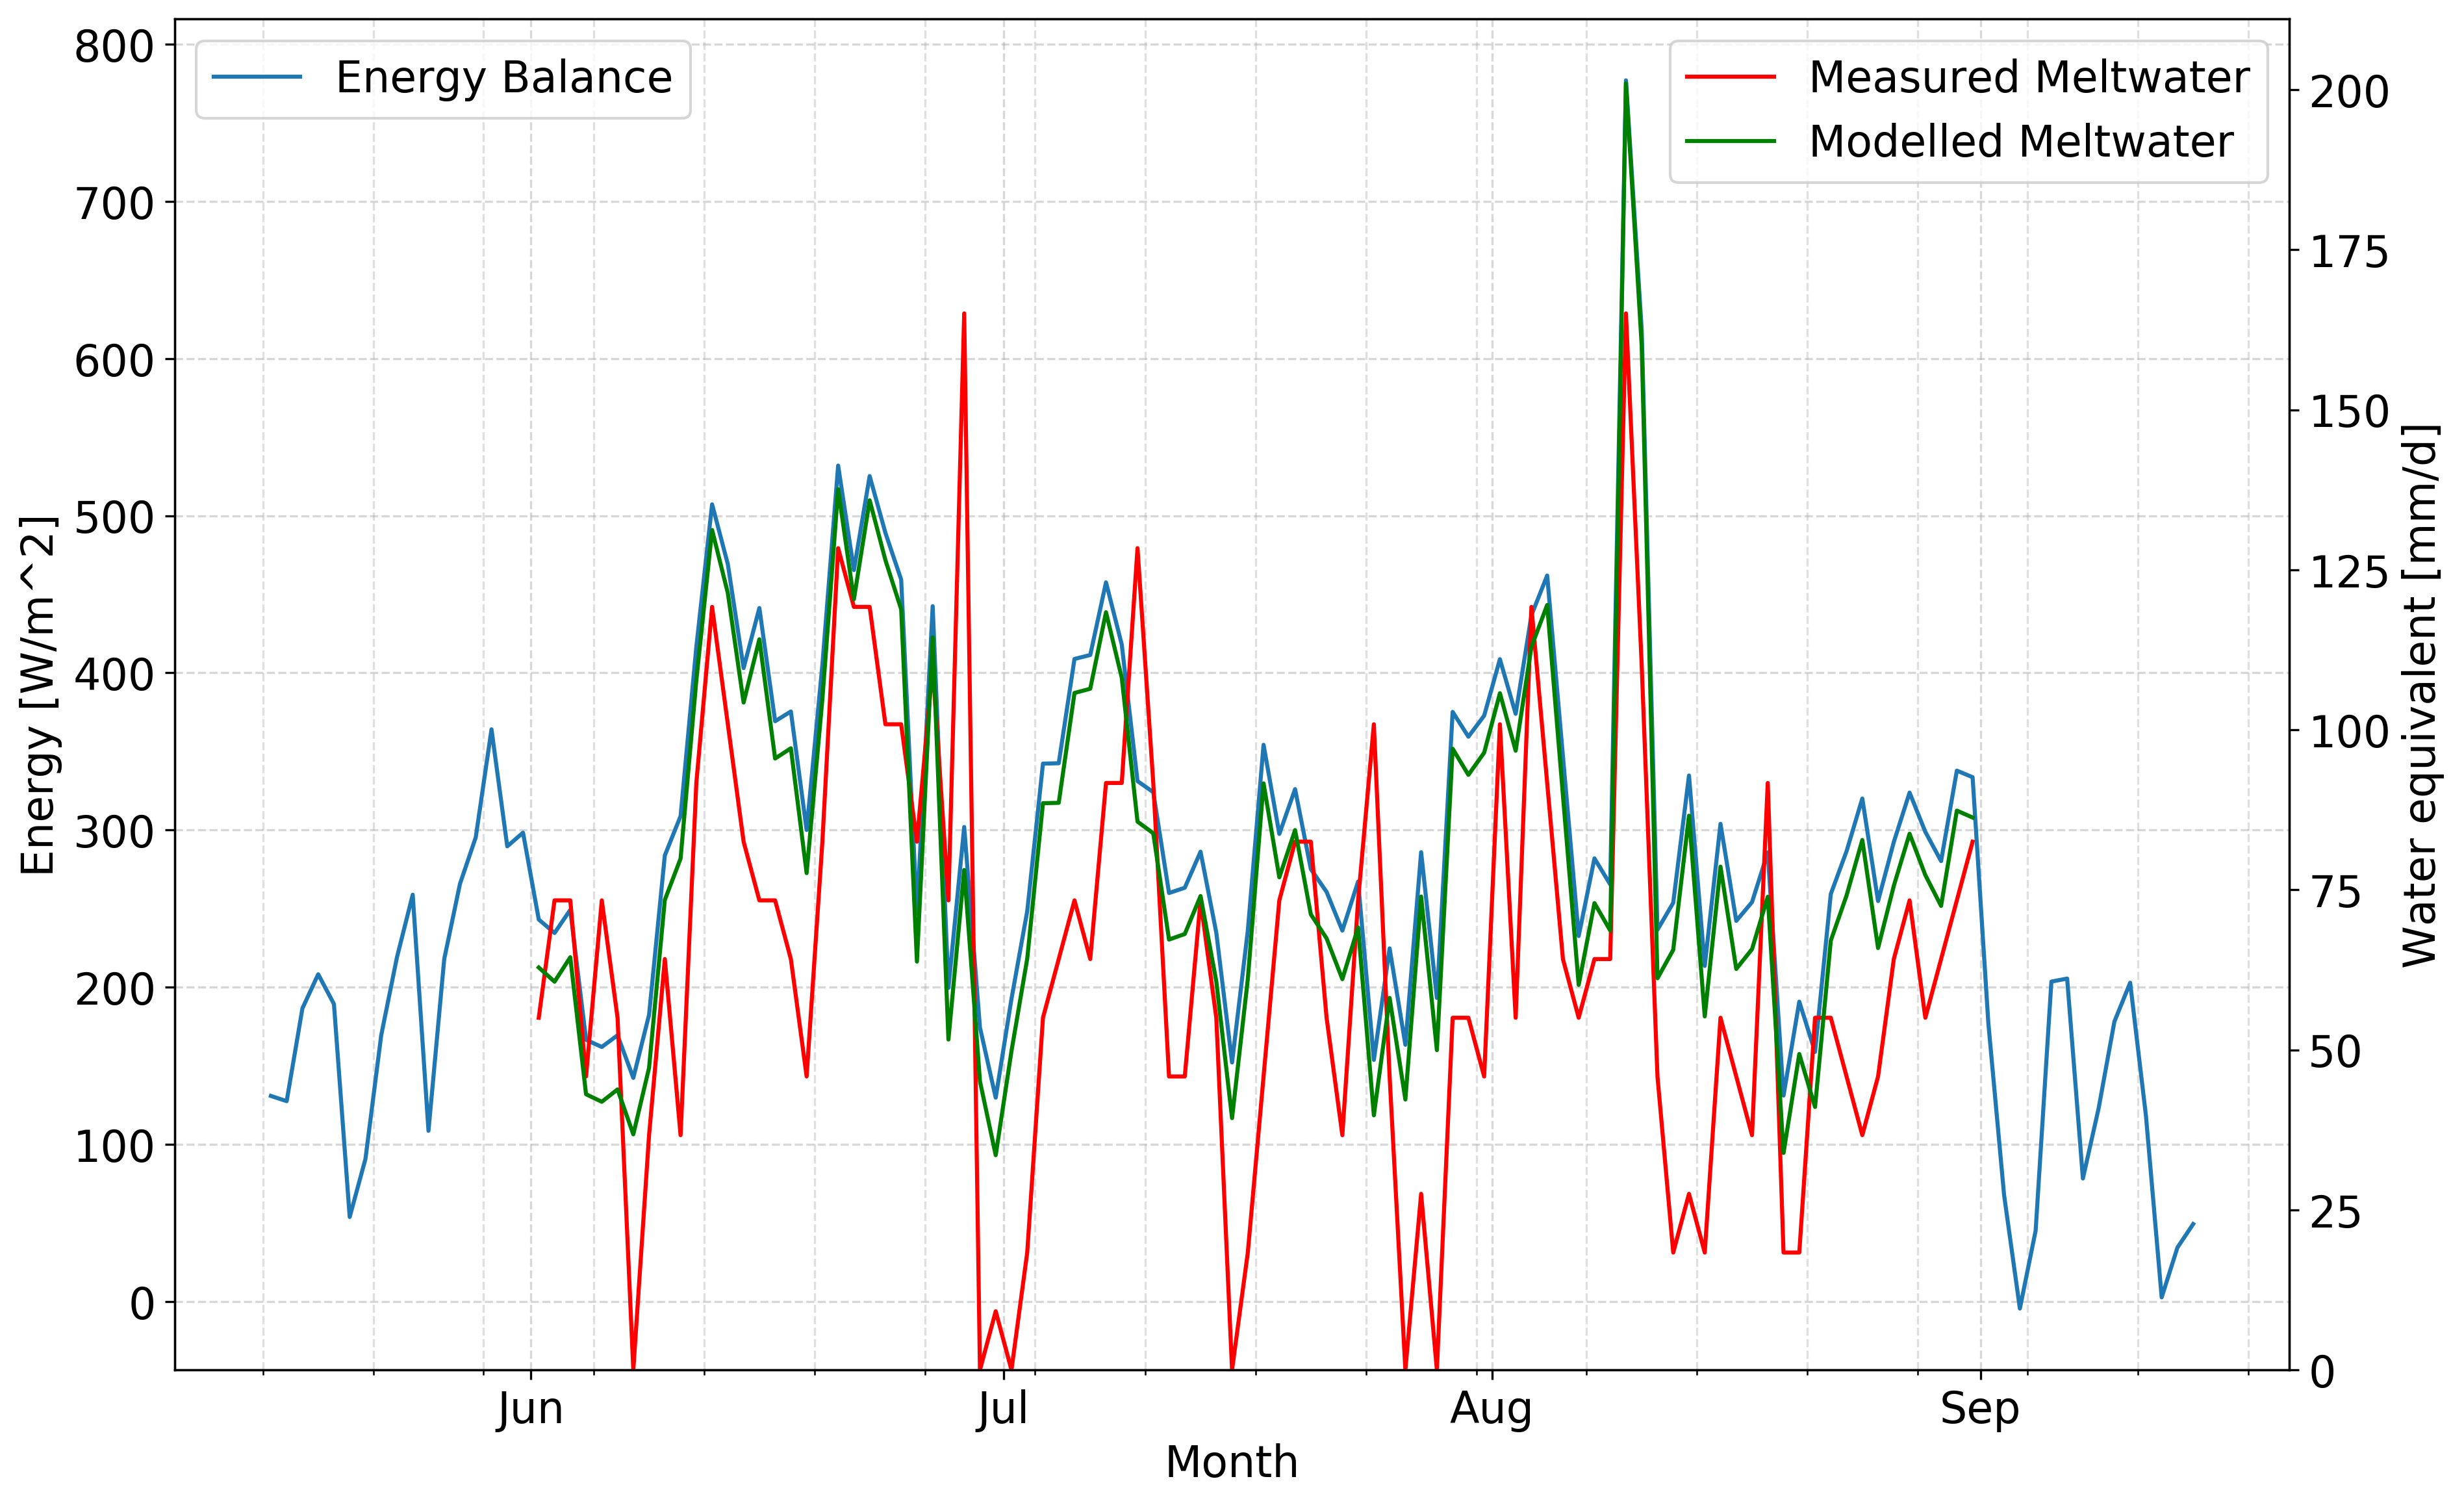
\includegraphics[width=\resultplotsize\textwidth]{../Software/plots/Total_energy_balance_summed_with_water_equivalent_2017.png}
\caption[Energiebilanz inklusive der in Wasseräquivalent umgerechneten Ablation und dem modellierten Schmelzwasser, Ablationsgebiet Pasterze im Zeitraum Sommer 2017, Tagesmittel]{Energiebilanz inklusive der in Wasseräquivalent umgerechneten Ablation und dem modellierten Schmelzwasser, Ablationsgebiet Pasterze im Zeitraum Sommer 2017, Tagesmittel (Quelle: eigene Darstellung)}
\label{fig:Energiebilanz im Sommer 2017 inklusive der in Wasseräquivalent umgerechneten Ablation und dem modellierten Schmelzwasser}
\end{figure}

\begin{figure}[H]
\centering
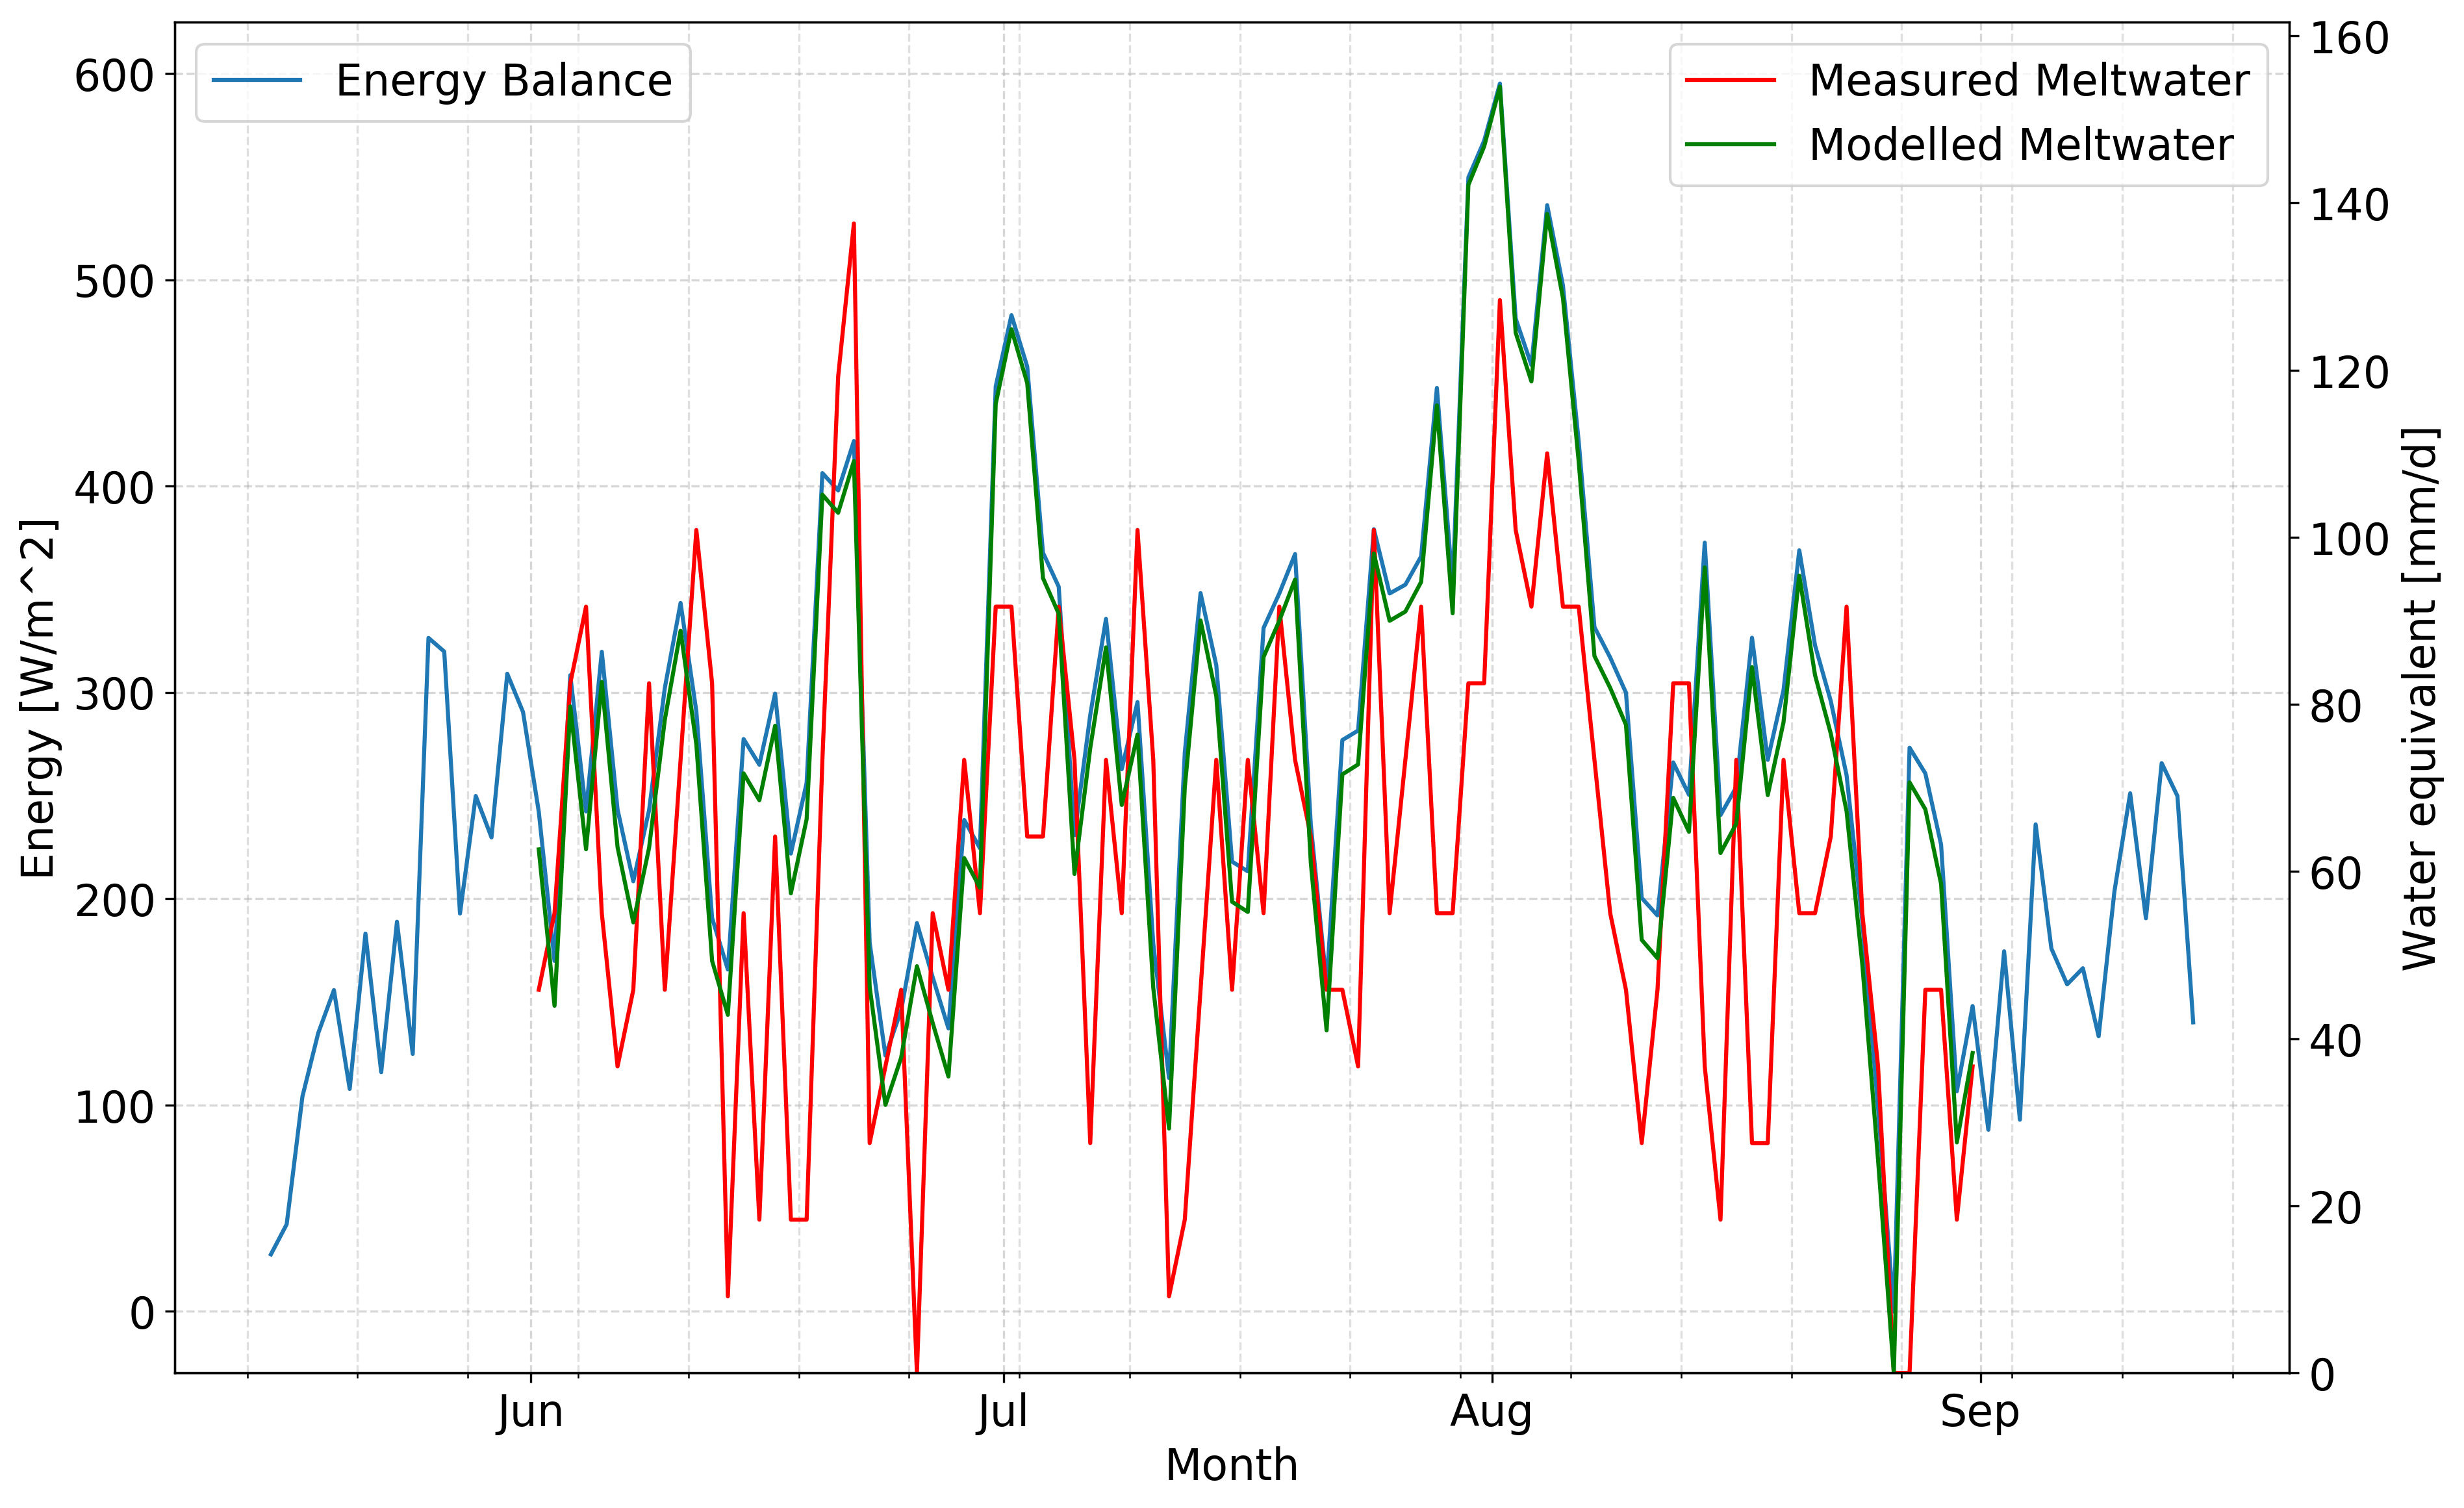
\includegraphics[width=\resultplotsize\textwidth]{../Software/plots/Total_energy_balance_summed_with_water_equivalent_2018.png}
\caption[Energiebilanz inklusive der in Wasseräquivalent umgerechneten Ablation und dem modellierten Schmelzwasser, Ablationsgebiet Pasterze im Zeitraum Sommer 2018, Tagesmittel]{Energiebilanz inklusive der in Wasseräquivalent umgerechneten Ablation und dem modellierten Schmelzwasser, Ablationsgebiet Pasterze im Zeitraum Sommer 2018, Tagesmittel (Quelle: eigene Darstellung)}
\label{Energiebilanz im Sommer 2018 inklusive der in Wasseräquivalent umgerechneten Ablation und dem modellierten Schmelzwasser}
\end{figure}


Abbildung \ref{Vergleich modelliertes und gemessenes Schmelzwasser} stellt  anhand eines Scatter-Plots das modellierte und gemessene Schmelzwasser unmittelbar gegenüber. Im Idealfall liegen dabei alle Punkte auf der ``Line of unity'', deren Steigung $45^\circ$ beträgt. Der lineare Trend ist im Falle dieser Darstellung deutlich ersichtlich, allerdings beträgt die Steigung der Regressionsgeraden nur ca $28^\circ$ und sie schneidet die y-Achse ca. beim Wert 40 [mm/d]. Dies bedeutet einerseits, dass das Modell bei sehr niedrigen gemessenen Werten für die Wasseräquivalenz bereits deutlich höhere Werte prädiziert und andererseits, dass tendenziell im Vergleich zum Gemessenen eher zu viel Schmelzwasser modelliert wird.

\begin{figure}[H]
\centering
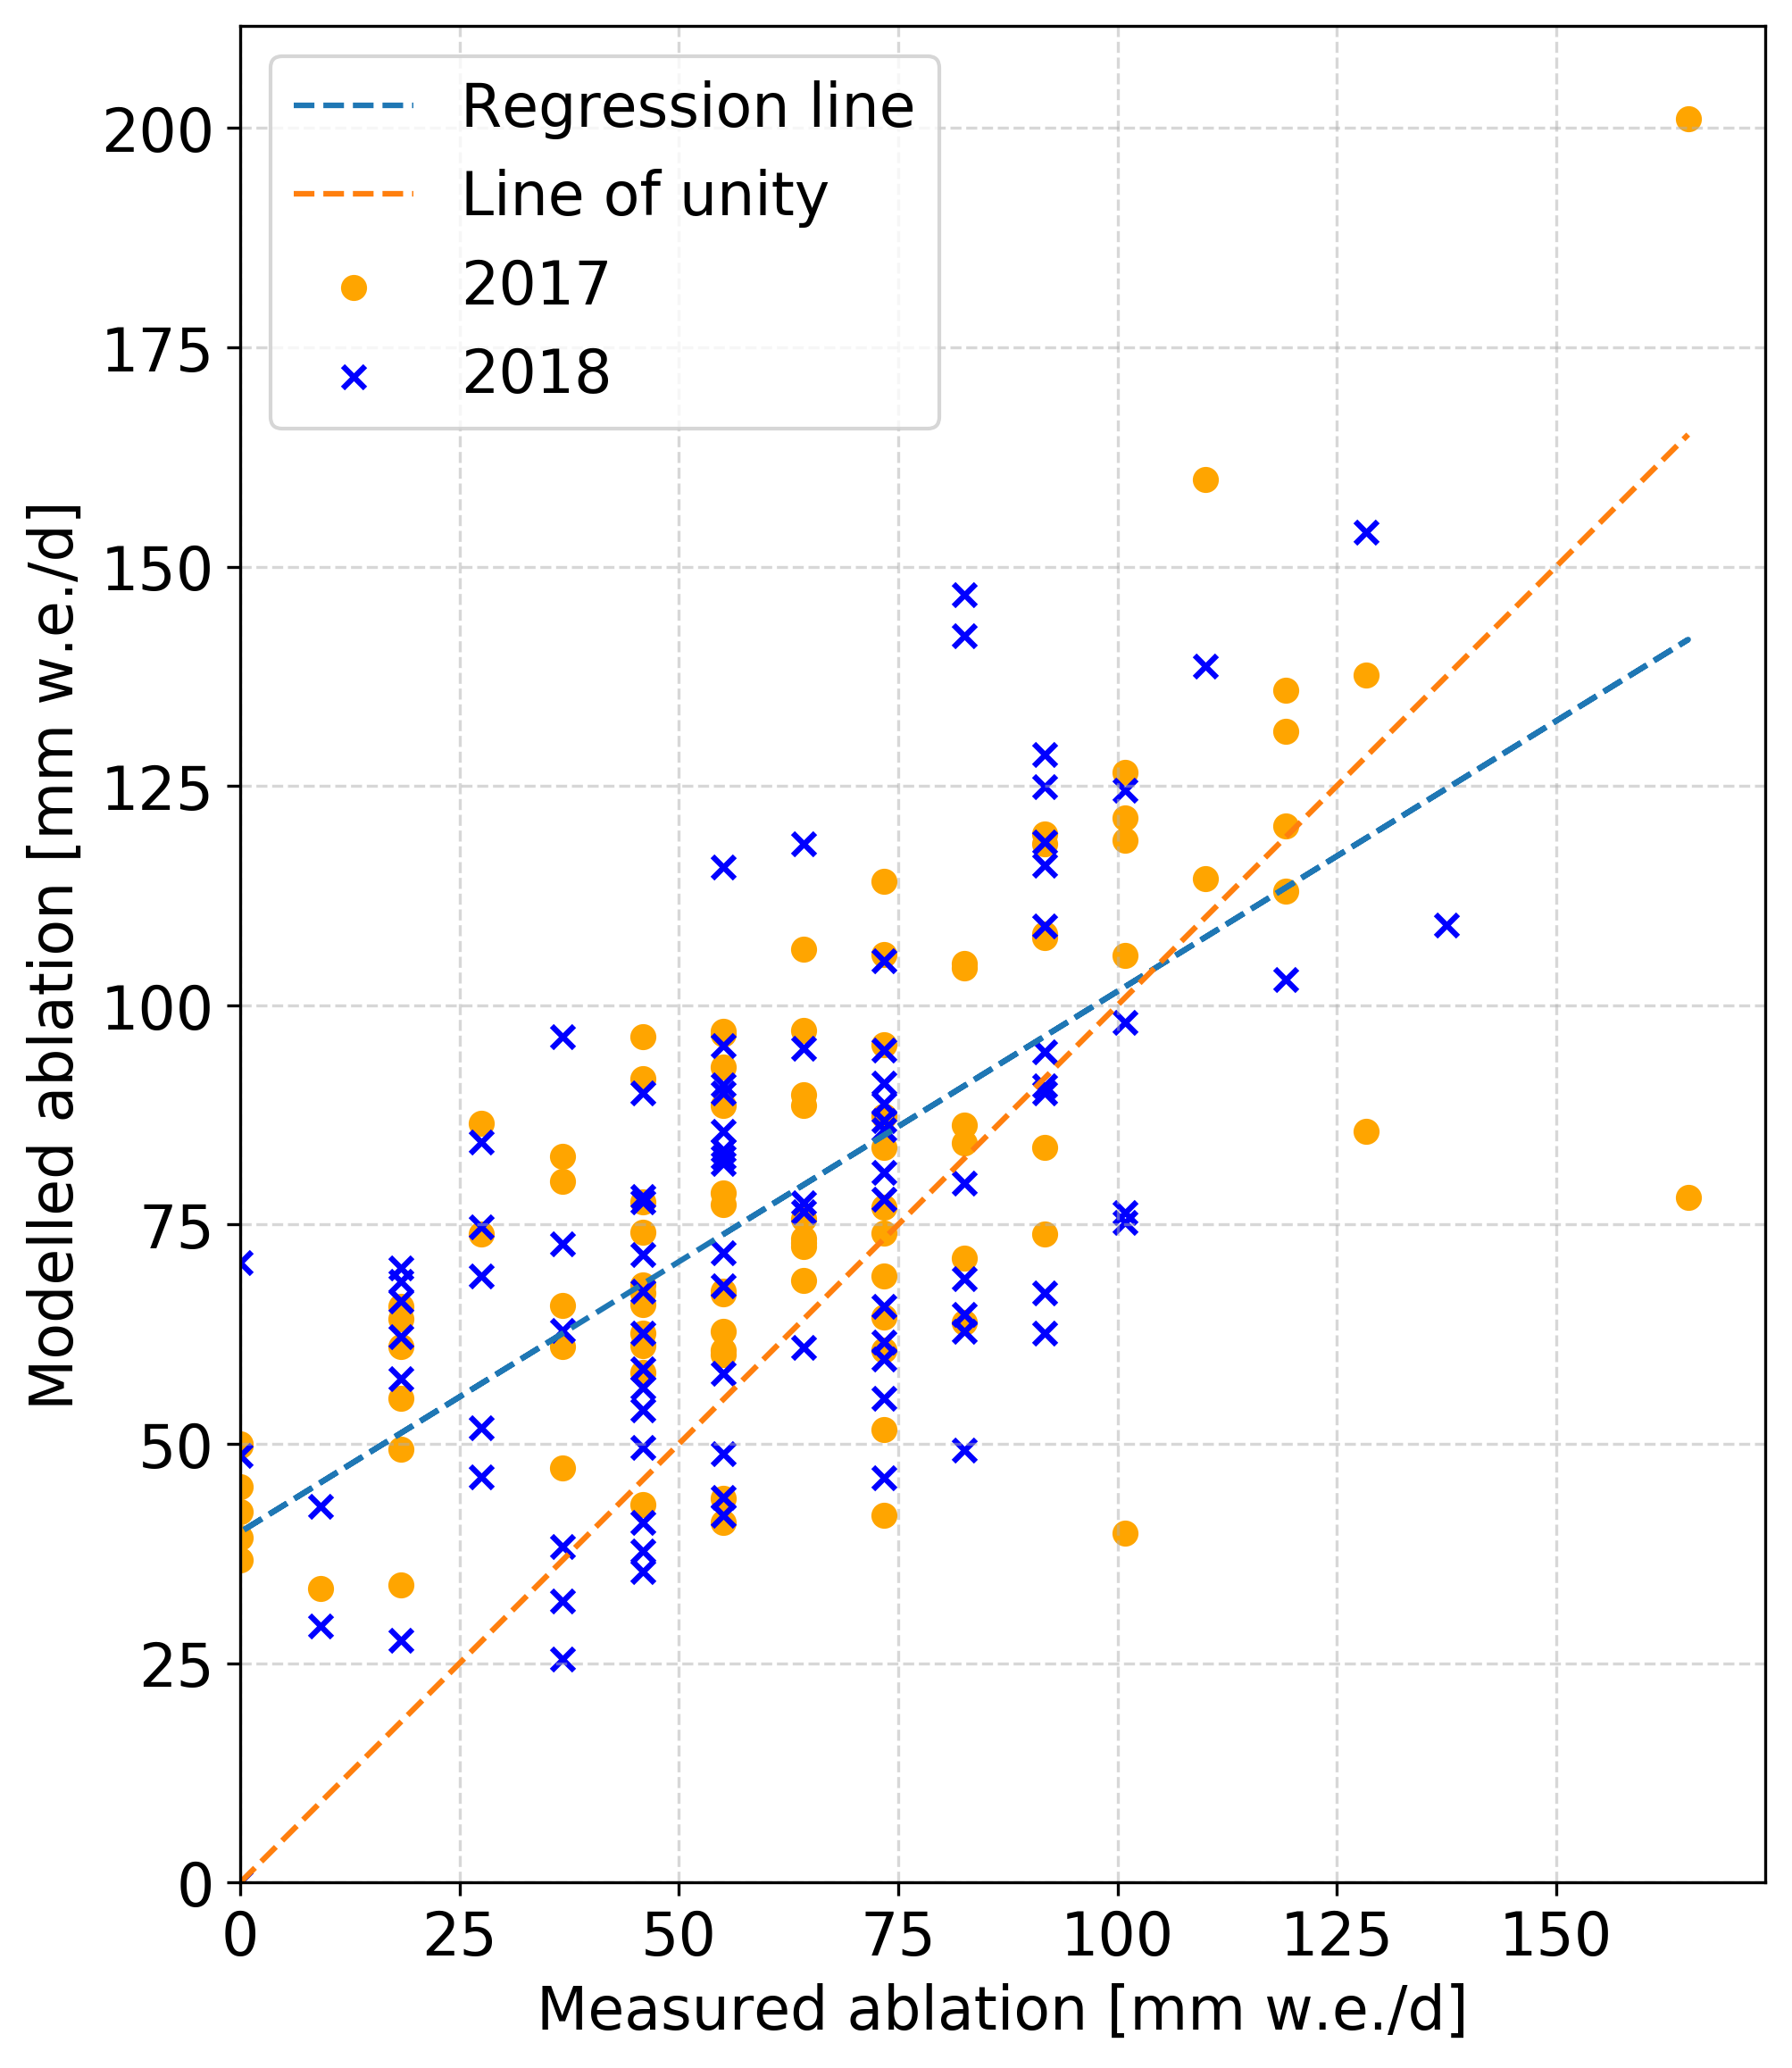
\includegraphics[width=0.6\textwidth]{../Software/plots/Scatter_measured_and_modelled_water_equivalent.png}
\caption[Vergleich modelliertes und gemessenes Schmelzwasser, Ablationsgebiet Pasterze im Zeitraum 2017 und 2018]{Vergleich modelliertes und gemessenes Schmelzwasser, Ablationsgebiet Pasterze im Zeitraum 2017 und 2018 (Quelle: eigene Darstellung)}
\label{Vergleich modelliertes und gemessenes Schmelzwasser}
\end{figure}



\subsection{Änderung des Eisdickenverlustes}
\subsubsection{``global dimming'' bzw. ``global brightening''}
Da das theoretische Modell der Energiebilanz und das daraus folgende Schmelzwasser gut mit der Realität übereinstimmt, können auch weitere Analysen über Veränderung der Energiebilanz durch ``global dimming'' und ``global brightening'' und dessen Auswirkung auf das Schmelzwasser vorgenommen werden. Um die Veränderung greifbarer zu machen, wird das Schmelzwasser, wie in der Durchführung beschrieben, in Eisdickenverlust umgerechnet.\\

Für diese Analyse wird wieder das Jahr 2018 von 1. Juni bis 1. September (siehe Abbildung \ref{Energiebilanz im Sommer 2018 inklusive der in Wasseräquivalent umgerechneten Ablation und dem modellierten Schmelzwasser}) verwendet. In diesem Zeitraum ergibt sich ein gemessener Gesamteisdickenverlust von $5.99~m$ und ein modellierter von $7.59~m$. Es spiegelt sich die Erkenntnis aus Abbildung \ref{Vergleich modelliertes und gemessenes Schmelzwasser} wieder, wo festgestellt wurde, dass tendenziell im Vergleich zum Gemessenen zu viel Schmelzwasser modelliert wird. Bei der Simulation von ``global dimming'' und ``global brightening'' wird die Veränderung dieses Eisdickenverlustes im Modell untersucht. Damit diese Änderungen so gut wie möglich der Realität entsprechen, werden alle Änderung noch mit dem Faktor $5.99/7.59$ multipliziert. Das Ergebnis ist in Tabelle \ref{tab:Auswirkung von global dimming oder global brightening auf den Eisdickenverlust innerhalb vom 1. Juni bis 1. September im Jahr 2018} zusammengefasst.

\begin{table}[H]
\centering
\setstretch{1.3} 
\caption{Auswirkung von global dimming oder global brightening auf den Eisdickenverlust im Zeitraum vom 1. Juni bis 1. September im Jahr 2018}
\label{tab:Auswirkung von global dimming oder global brightening auf den Eisdickenverlust innerhalb vom 1. Juni bis 1. September im Jahr 2018}
\begin{tabular}{|l|c|c|c|c|c|}
\hline
Zusätzliche $W/m^2$       &  $-9$ & $-6$  & $-3$ & $0$ & $+3$ \\ \hline
Differenz {[}cm{]} & -18    & -12 & -6 & 0  & 6  \\ \hline
\end{tabular}
\end{table}

Es kann erkannt werden, dass sich ``global dimming'' und ``global brightening'' sehr wohl signifikant auf die Änderung der Eisdicke eines Gletschers im Ablationsgebiet auswirken. Bei knapp $10~W/m^2$ kleinerer Energiebilanz über  die Sommermonate ergibt sich bereits ein um $18~cm$ geringerer Eisdickenverlust. Der Zusammenhang ist linear und kann somit mit ca. $6~cm$ pro $3 W/m^2$ weiter fortgesetzt werden.\\

\subsubsection{``Greenhouse Gas Forcings''}
Eine weitere Untersuchung kann in dieser Hinsicht auch beim Thema der ``Greenhouse Gas forcings'' durchgeführt werden. Durch unterschiedliche Zusammensetzung der Atmosphäre verändert sich nämlich der Betrag der langwelligen Strahlung der von der Atmosphäre rückgestrahlt wird. Abbildung \ref{Globale Temperatur und ``Greenhouse Gas Forcings''} zeigt die ``Greenhouse Gas forcings'' zusammen mit der Temperatur seit dem Jahr 1900. 

\begin{figure}[H]
\centering
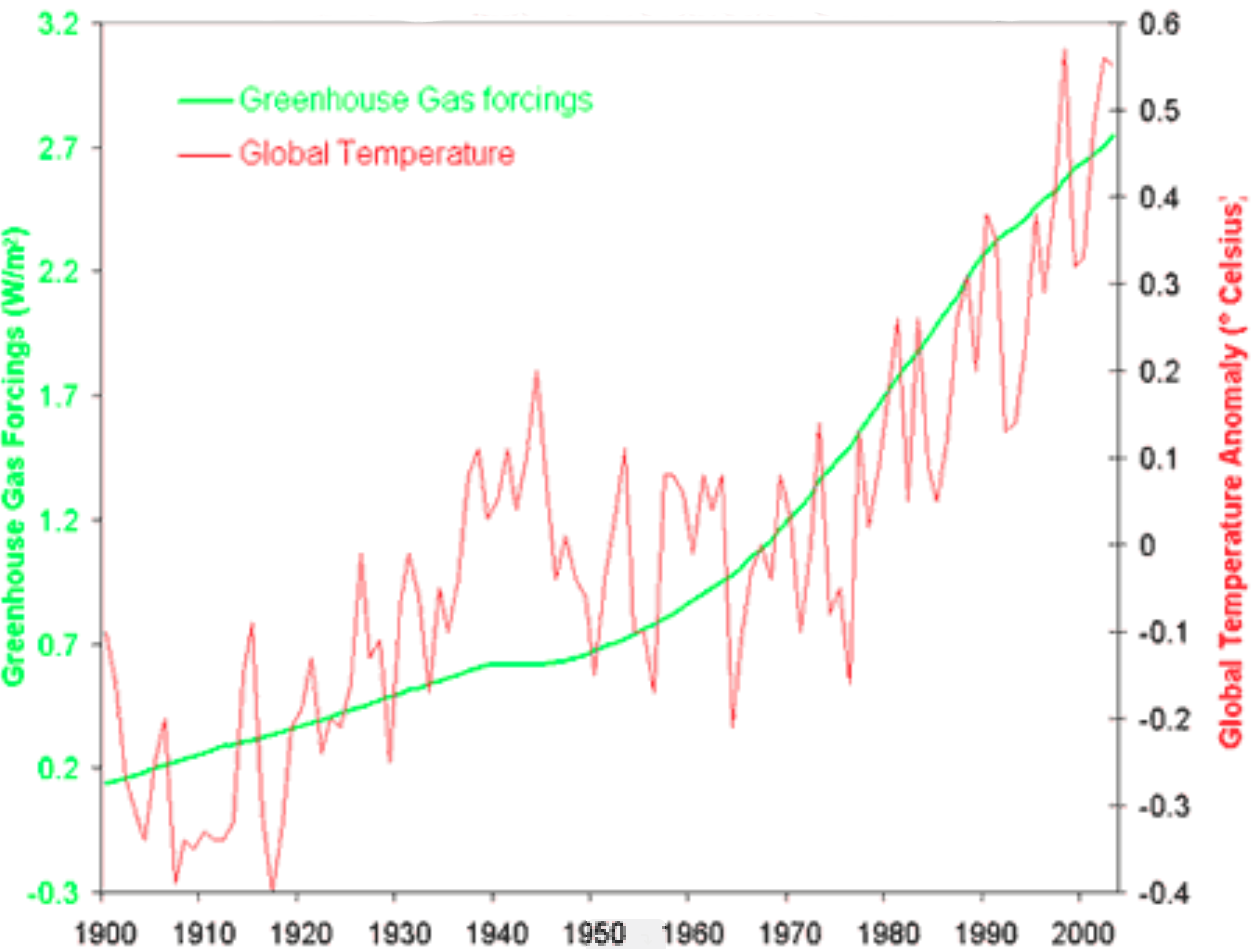
\includegraphics[width=0.8\textwidth]{pictures/greenhouse_gas_forcing.png}
\caption[Globale Temperatur und ``Greenhouse Gas Forcings'']{Globale Temperatur und ``Greenhouse Gas Forcings'' \parencite{GreenhouseGasForcing}}
\label{Globale Temperatur und ``Greenhouse Gas Forcings''}
\end{figure}


Mithilfe der errechneten Differenzen aus Tabelle \ref{tab:Auswirkung von global dimming oder global brightening auf den Eisdickenverlust innerhalb vom 1. Juni bis 1. September im Jahr 2018} kann errechnet werden, um wie viel sich die Eisdicke im Ablationsgebiet in etwa insgesamt weniger verringert hätte, wäre die langwellige einkommende Strahlung seit 1900 konstant geblieben. Dabei werden allerdings alle anderen Komponenten wie Temperatur usw. nicht berücksichtigt. Dies gilt somit nur als grober Schätzwert. Außerdem wird immer nur der Zeitraum zwischen 1. Juni und 1. September betrachtet. Tendenziell ist somit der errechnete Wert im Absolutbetrag zu klein.\\

Zur Berechnung wird weiters eine lineare Veränderung der langwelligen eingehenden Strahlung angenommen. Betrachtet wird der Zeitraum vom Jahr 1900 bis zum Jahr 2000. In diesen 100 Jahren nimmt die Strahlung laut der Abbildung um ungefähr $2.5$ $W/m^2$ zu.\\

Die Formel zur Berechnung kann durch
\begin{equation}
\Delta I =\sum_{i=1}^{100}\left ( \frac{a}{100}\cdot i \cdot b \right )
\end{equation}

angegeben werden, wobei $a=2.5\frac{W}{m^2}$ dem Greenhouse forcing in der betrachteten Zeit entspricht und $b=2 \frac{cm \cdot m^2}{W}$ (abgeleitet aus Tabelle \ref{tab:Auswirkung von global dimming oder global brightening auf den Eisdickenverlust innerhalb vom 1. Juni bis 1. September im Jahr 2018}) die Eisdickenänderung pro $W/m^2$ in den betrachteten Monaten Juli-August darstellt.\\

Als Ergebnis folgt mit $\Delta I = 252.5~cm$, dass in den betrachteten 100 Jahren die Eisdicke im Ablationsgebiet der Pasterze bei Betrachtung der Sommermonate um ca. $\mathbf{2.5~m}$ \textbf{weniger abgenommen} hätte, wenn die langwellige Strahlung seit dem Jahr 1900 konstant geblieben wäre.



\subsection{Periodische Trendelimination der Energiebilanz}

Wie bereits erwähnt, machen Trendeliminationen bei einer so kurzen Zeitreihe wenig Sinn. Trotzdem zeigt Abbildung \ref{fig:Trendelimination der Energiebilanz} das Ergebnis der periodischen Trendelimination der Messreihe. Ein Jahr an darstellbaren Daten fällt durch die verwendete Methode (siehe Kapitel \ref{Periodische Trendelimination}) dabei weg. Eine Interpretation der Darstellung macht aufgrund der kurzen Datenreihe wenig Sinn, allerdings erkennt man eine leichte Abnahme der Energiebilanz im Untersuchungszeitrum.

\begin{figure}[H]
\centering
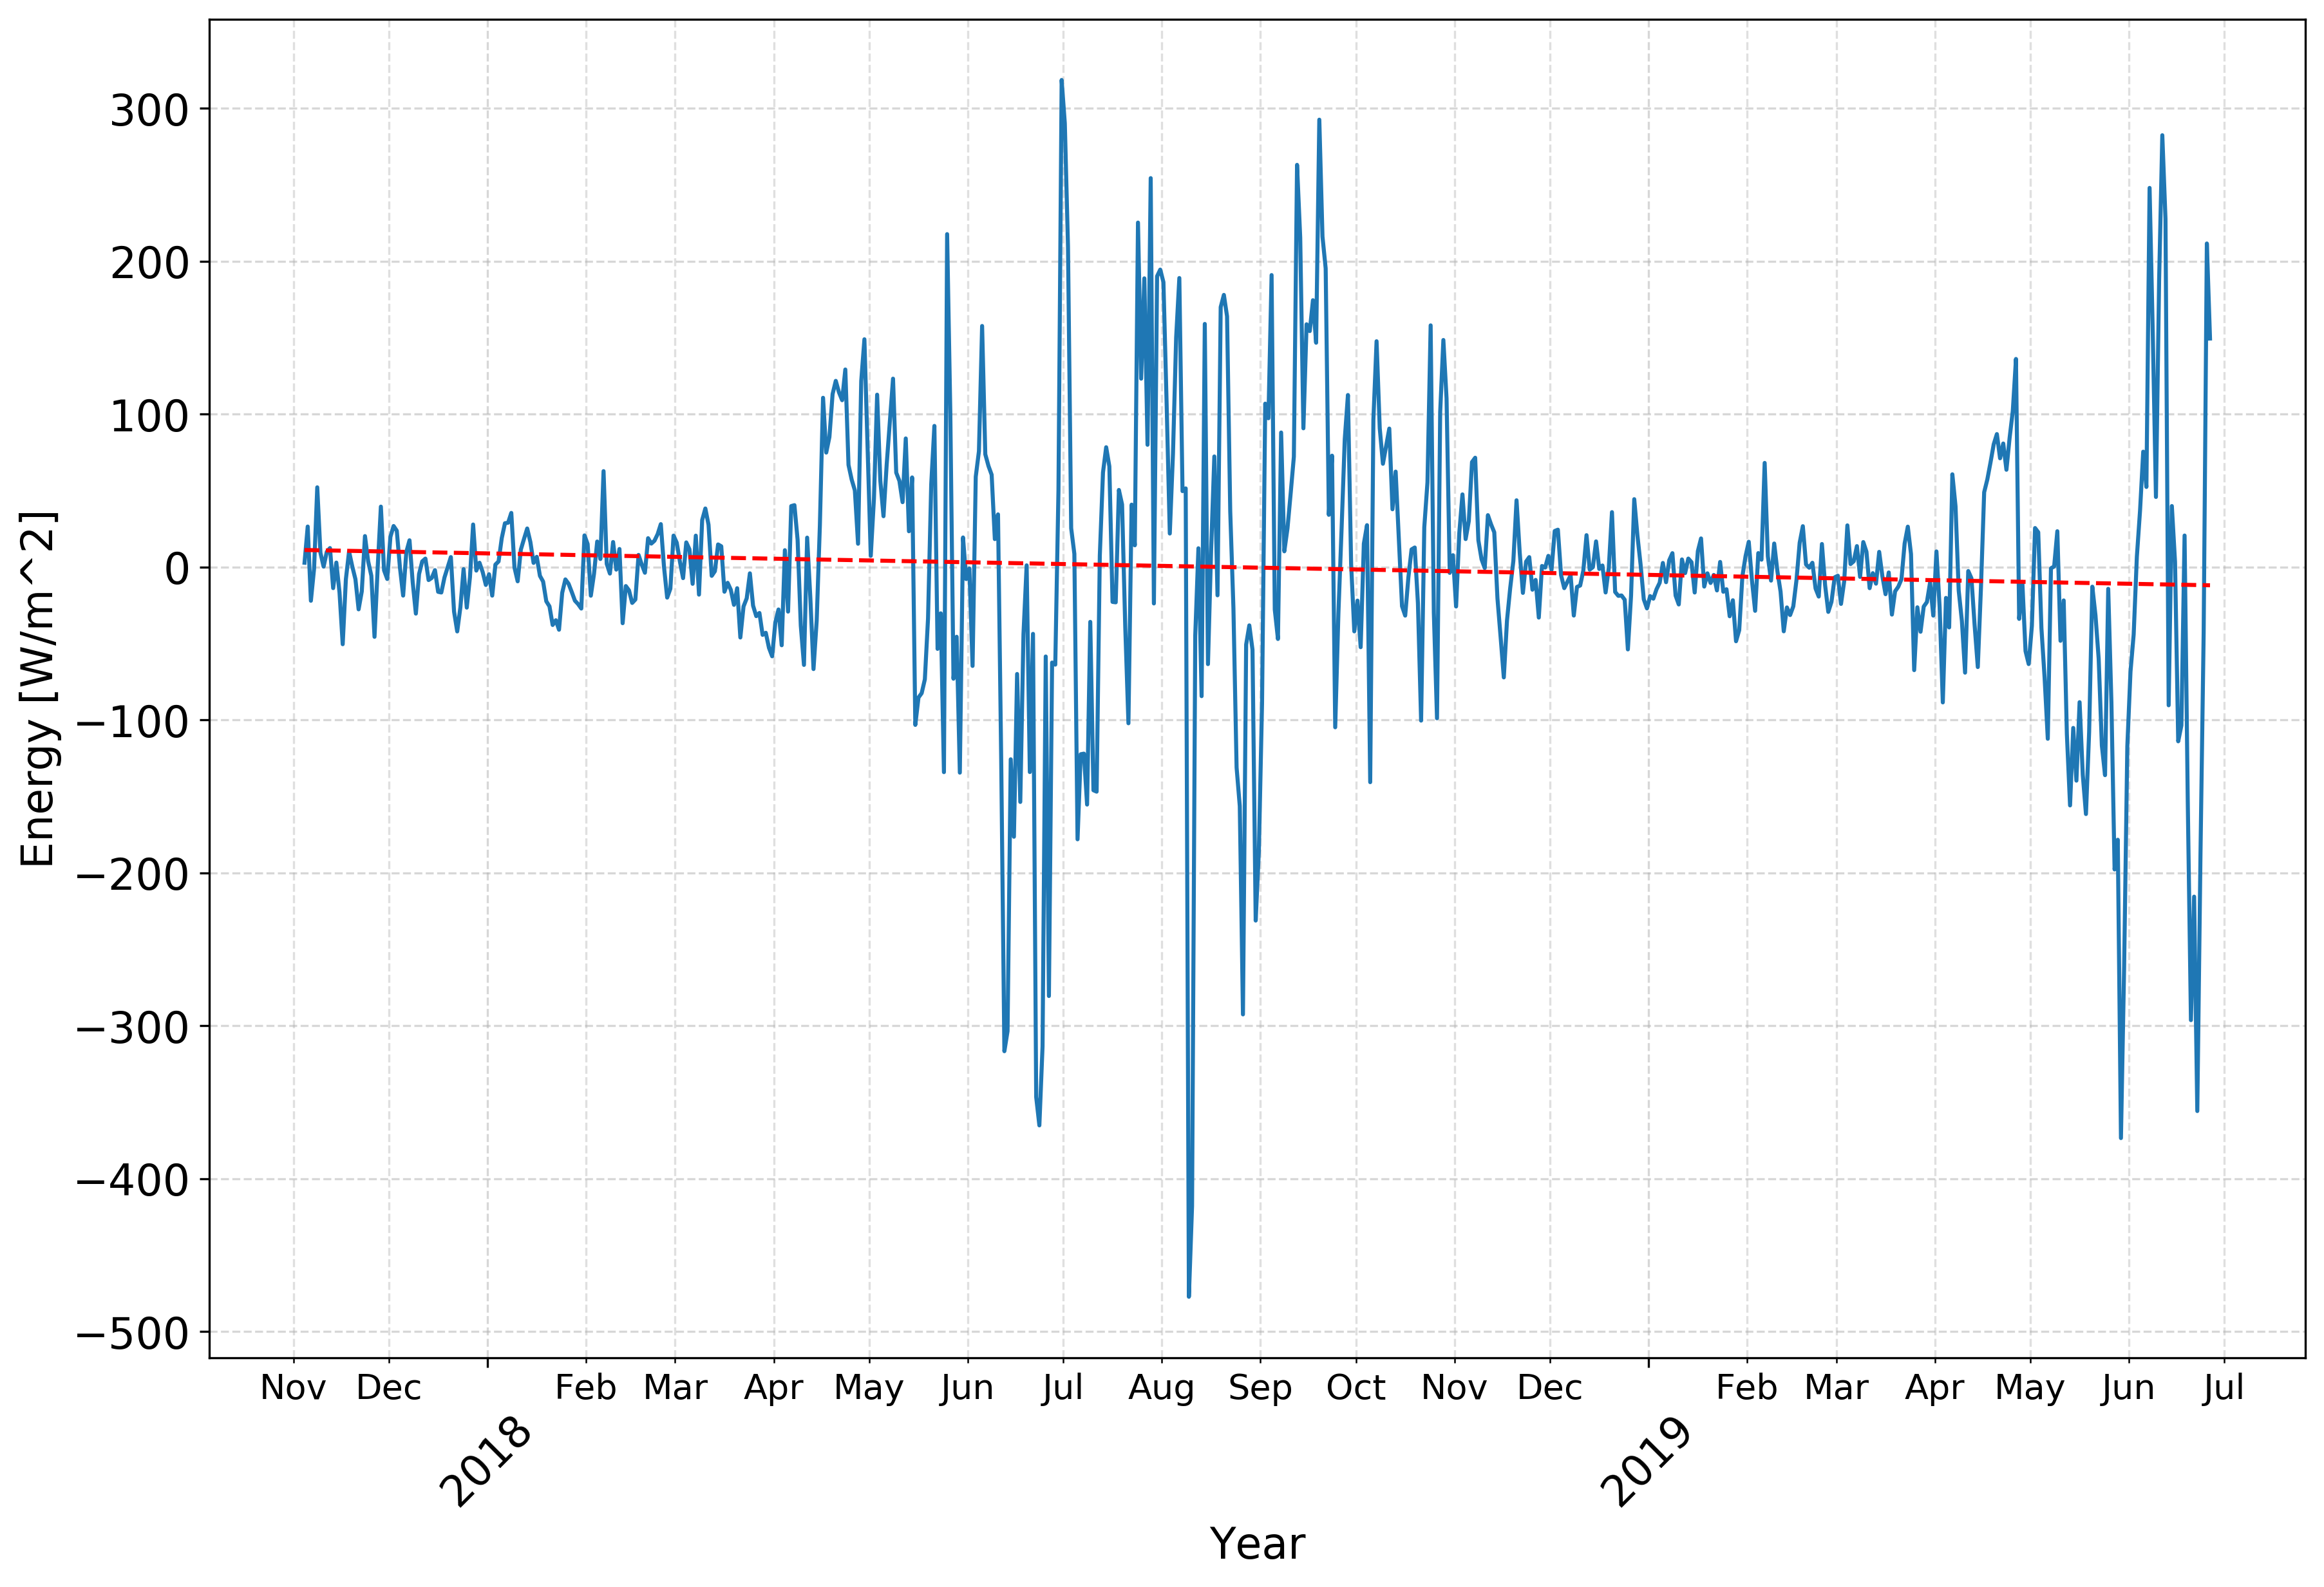
\includegraphics[width=\resultplotsize\textwidth]{../Software/plots/Total_energy_balance_summed_periodic_trend_eliminated.png}
\caption[Trendelimination der Energiebilanz, Ablationsgebiet Pasterze im Zeitraum November 2017 bis Juni 2019, Tagesmittel]{Trendelimination der Energiebilanz, Ablationsgebiet Pasterze im Zeitraum November 2017 bis Juni 2019, Tagesmittel (Quelle: eigene Darstellung)}
\label{fig:Trendelimination der Energiebilanz}
\end{figure}

Werden die Strahlungskomponente, sowie die der sensible und latente Wärmeeintrag der Energiebilanz separat betrachtet, kann erkannt werden, dass  die Abnahme aus der Strahlungskomponente resultiert. Die sensible und latente Wärme bleibt im Mittel über den betrachteten Zeitraum annähernd konstant.

\begin{figure}[H]
\centering
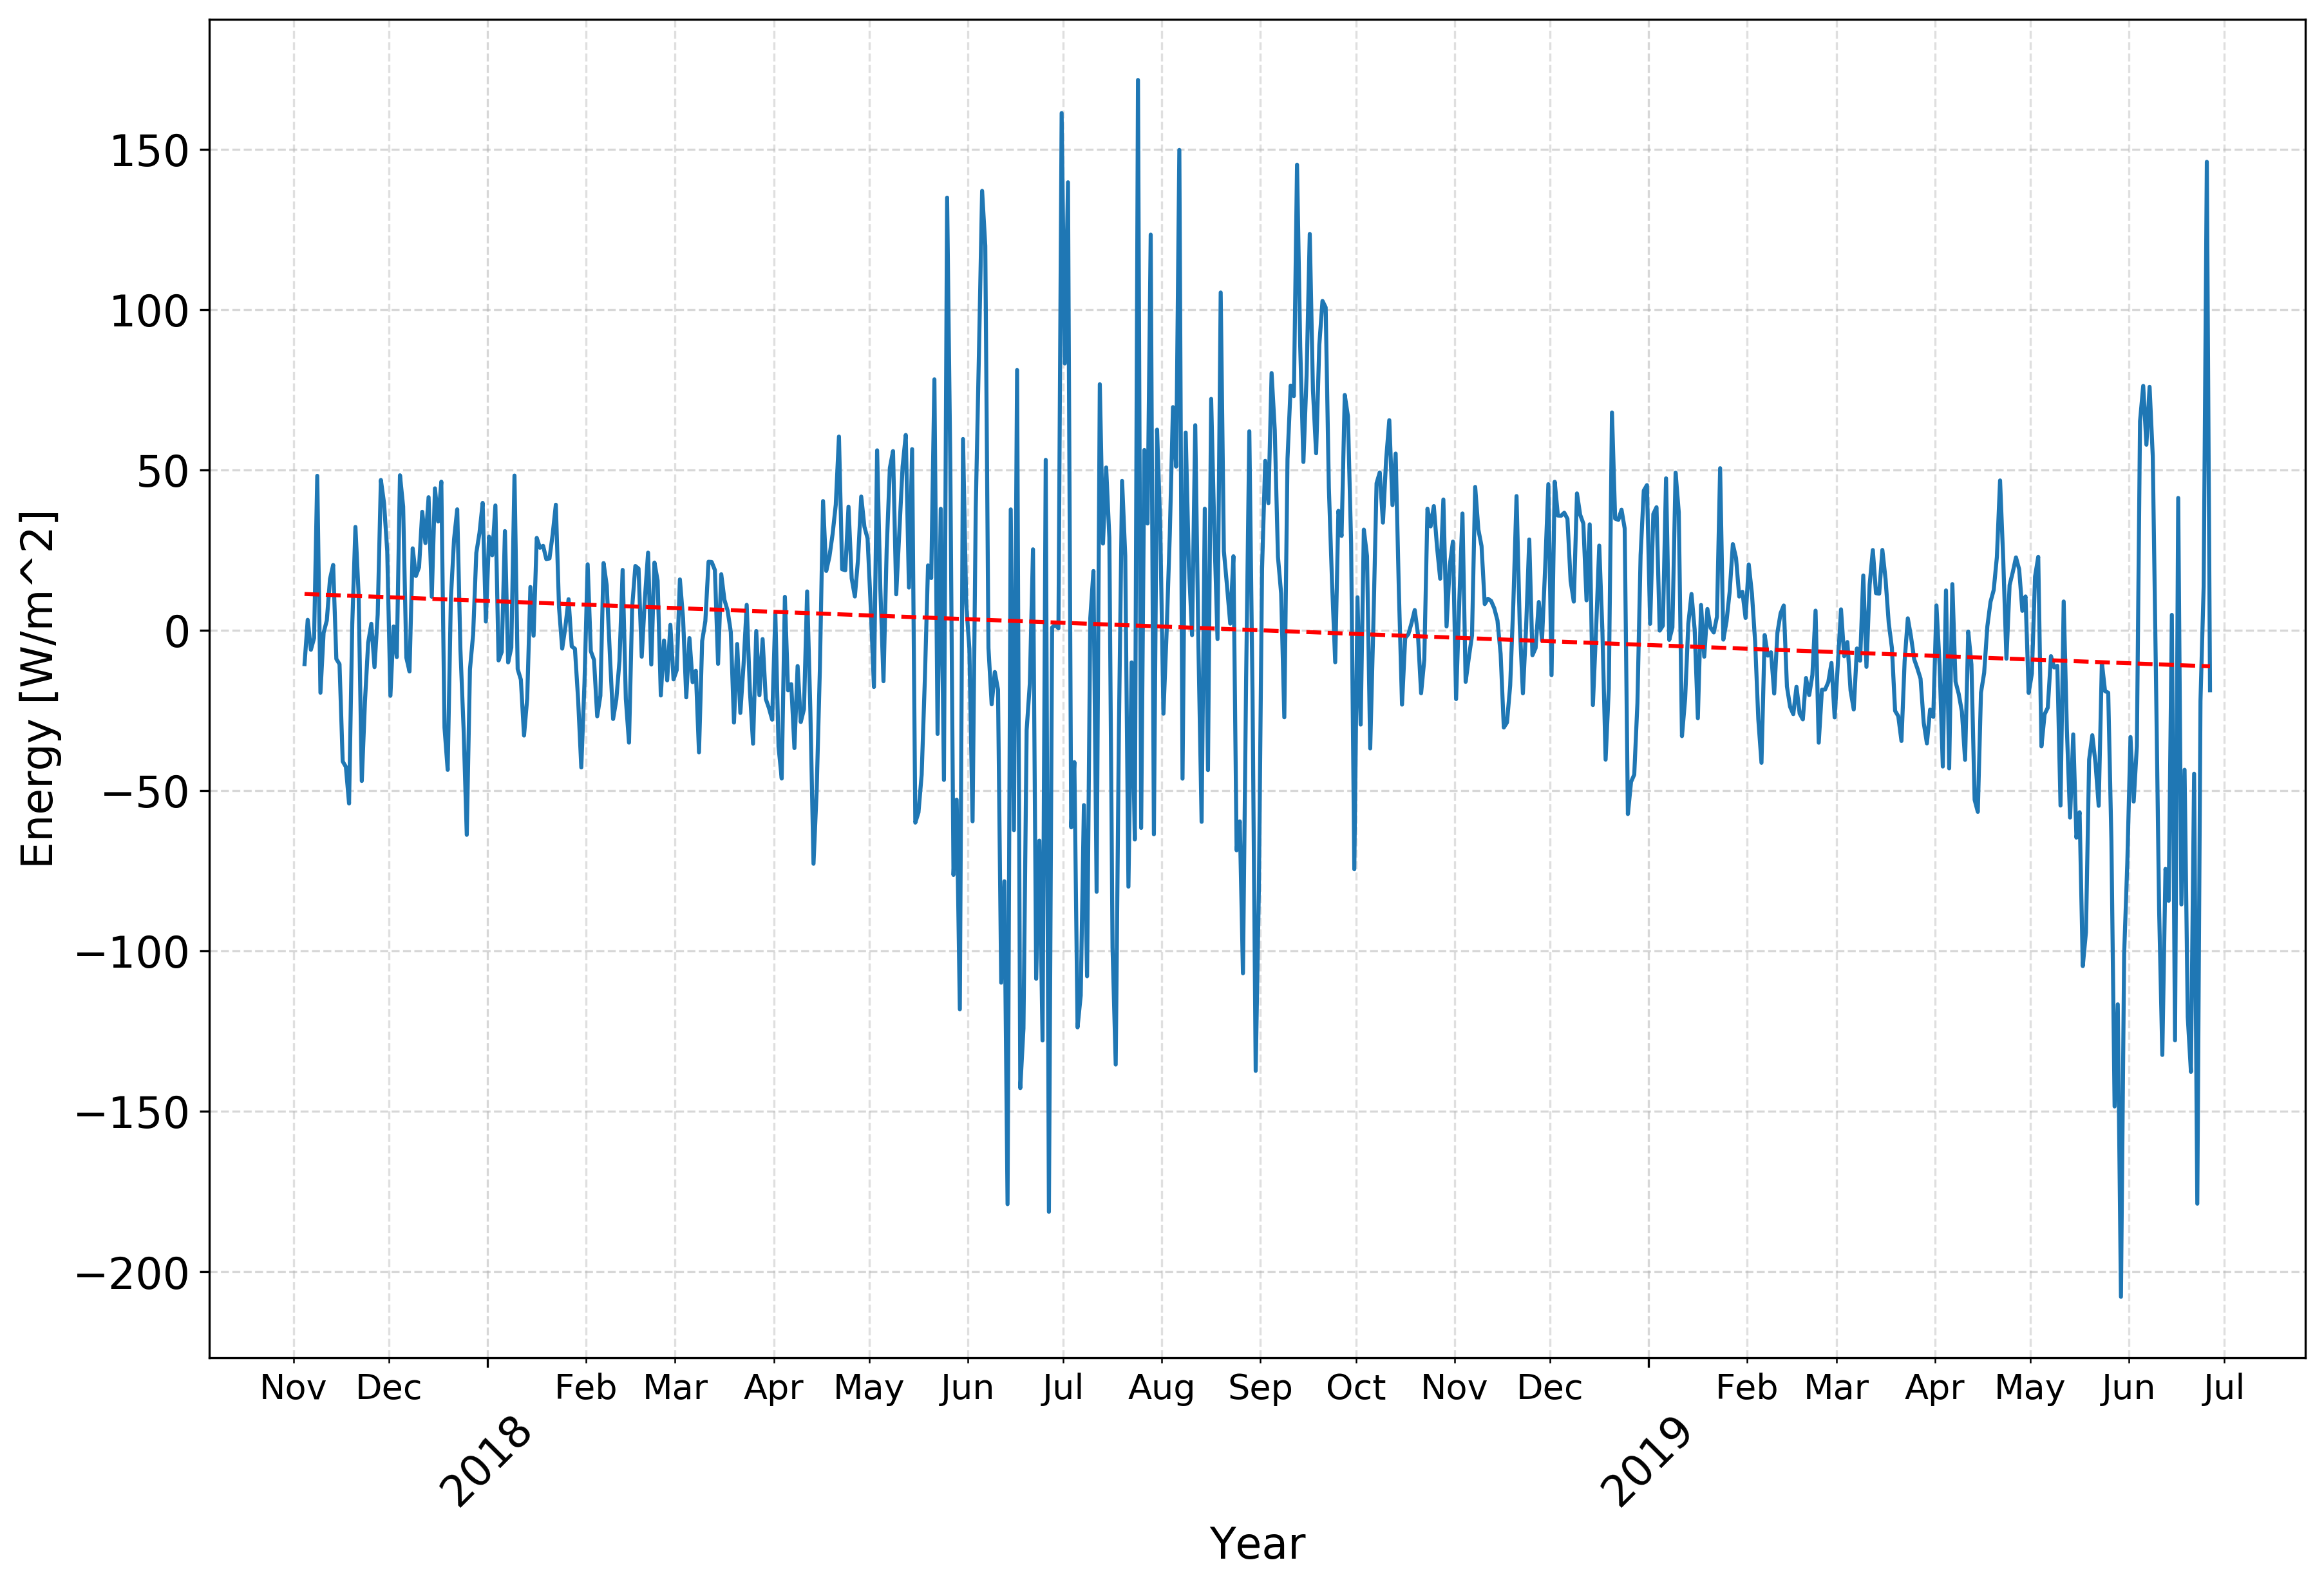
\includegraphics[width=\resultplotsize\textwidth]{../Software/plots/Radiation_summed_periodic_trend_eliminated.png}
\caption[Trendelimination der Strahlungskomponente der Energiebilanz, Ablationsgebiet Pasterze im Zeitraum November 2016 bis Juni 2019, Tagesmittel]{Trendelimination der Strahlungskomponente der Energiebilanz, Ablationsgebiet Pasterze im Zeitraum November 2016 bis Juni 2019, Tagesmittel (Quelle: eigene Darstellung)}
\label{fig:Trendelimination der Strahlungskomponente der Energiebilanz}
\end{figure}

\begin{figure}[H]
\centering
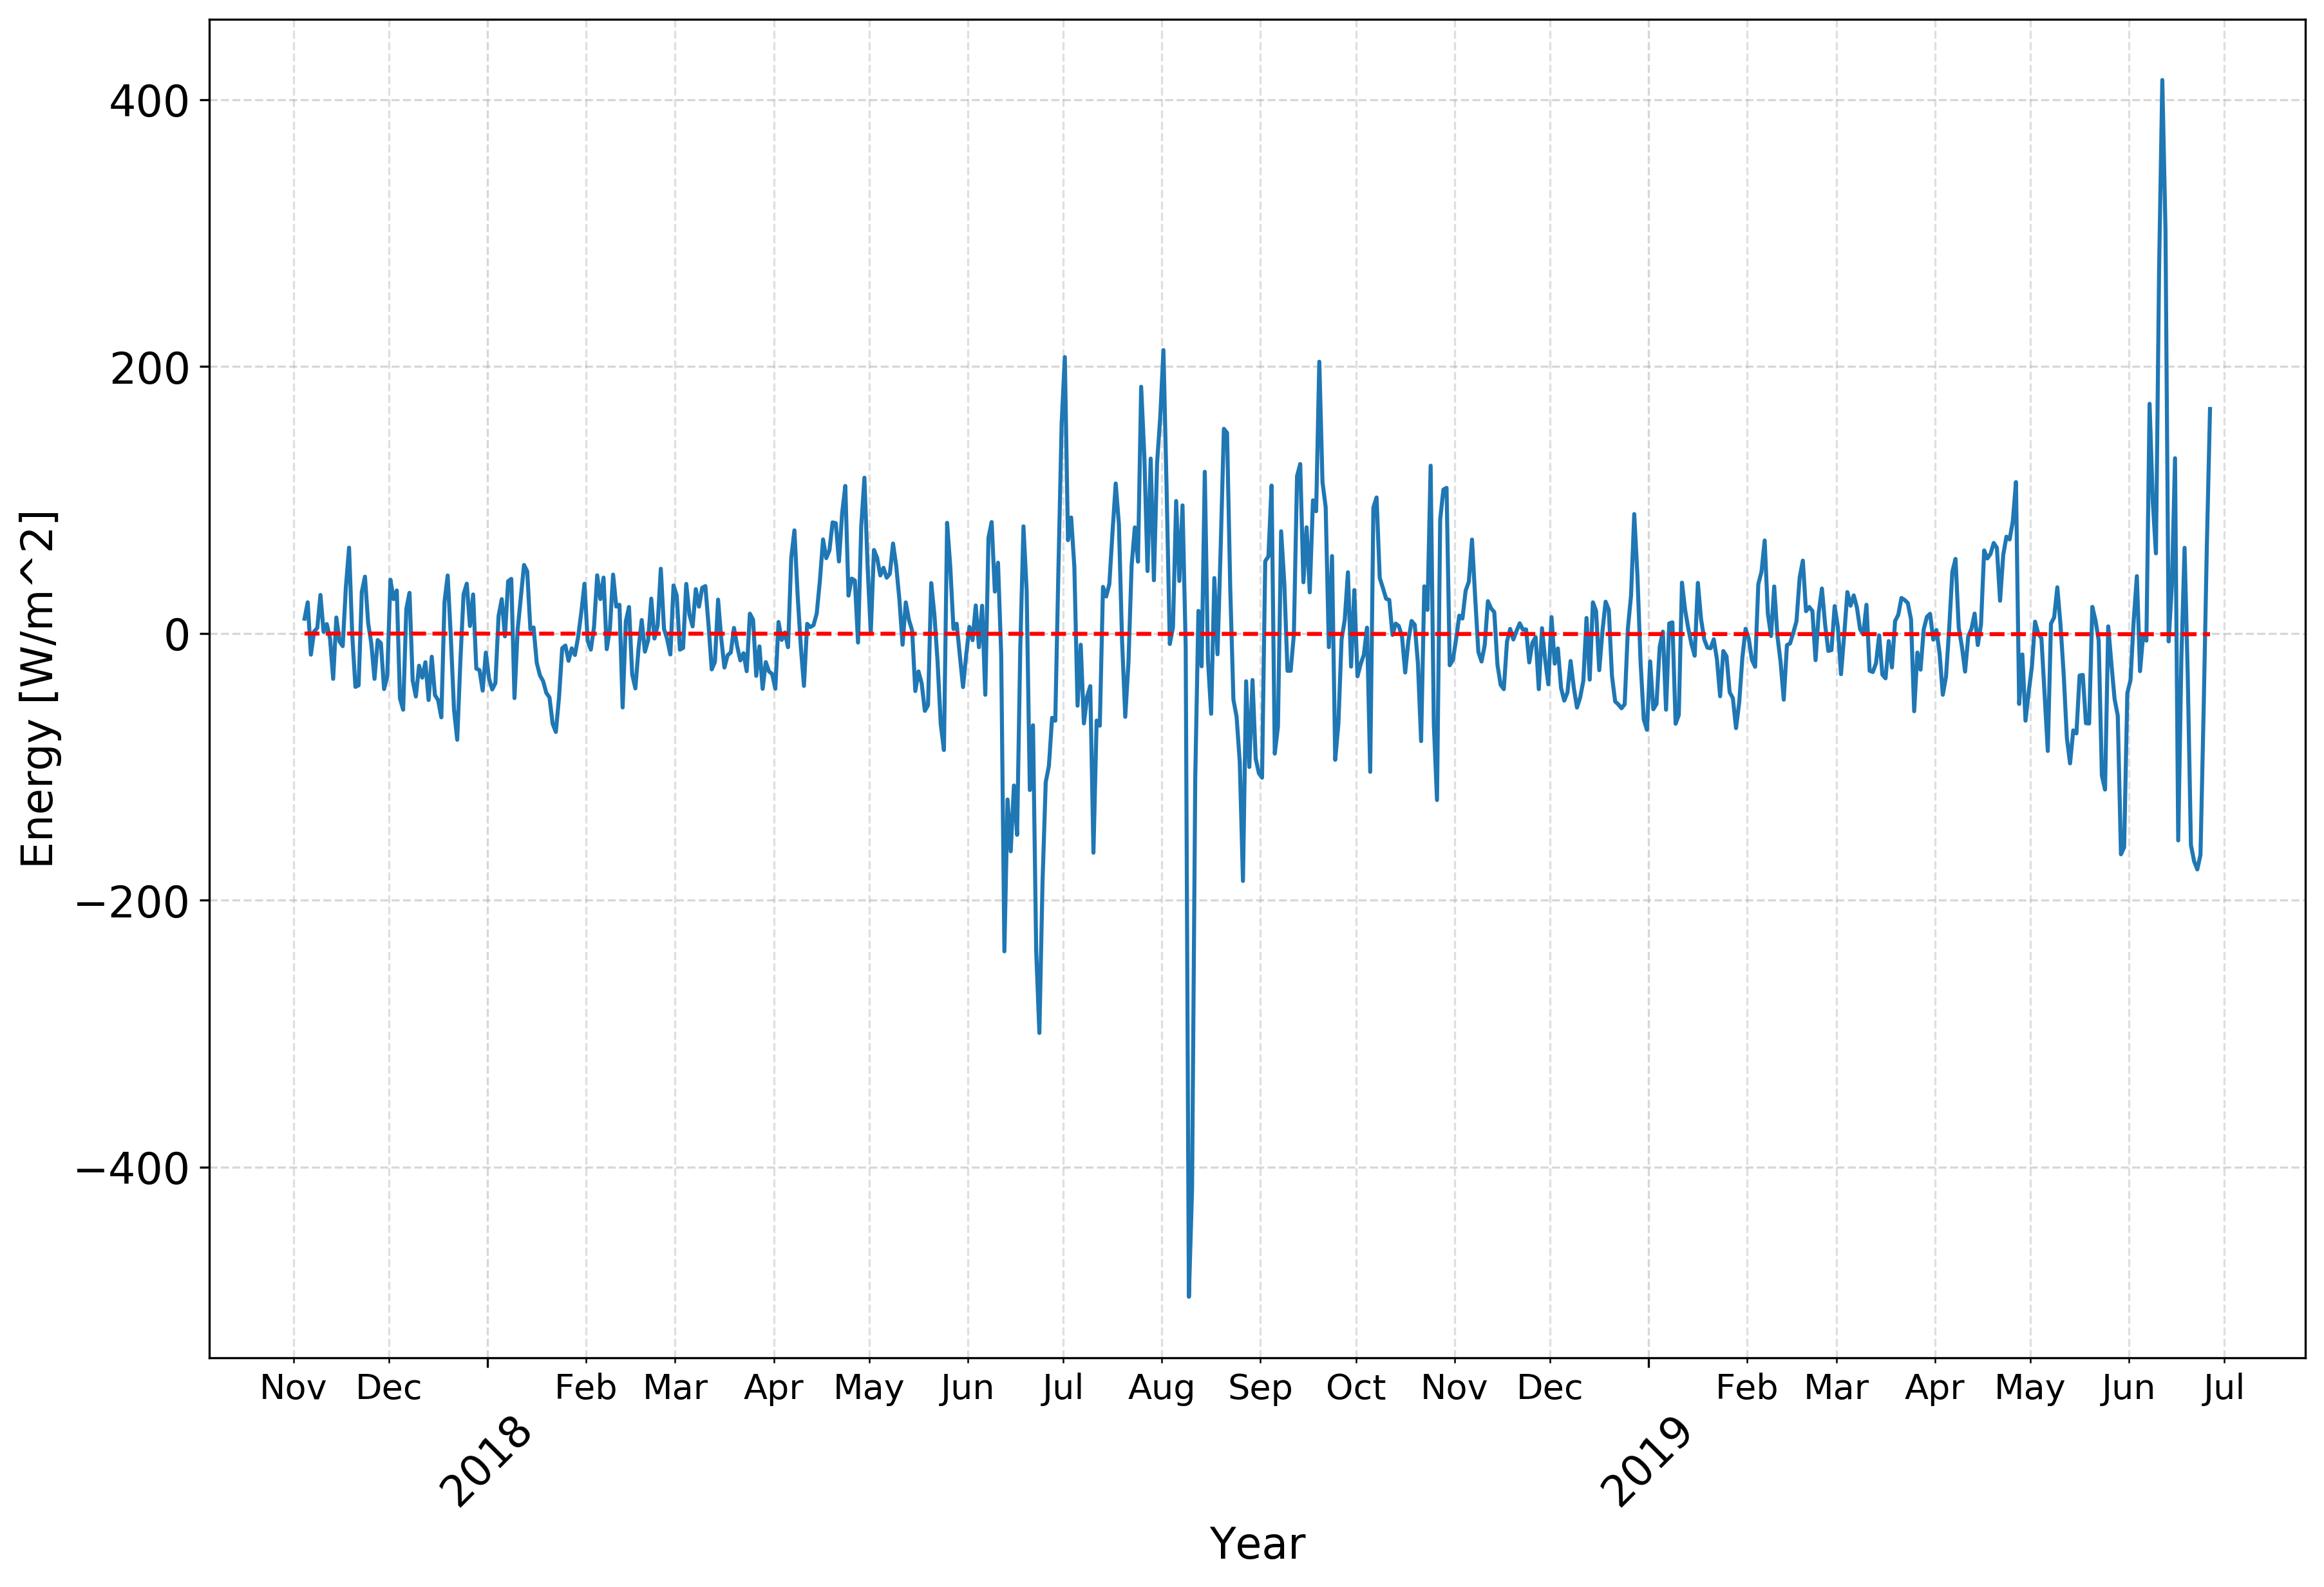
\includegraphics[width=\resultplotsize\textwidth]{../Software/plots/Latent_and_Sensible_summed_periodic_trend_eliminated.png}
\caption[Trendelimination der sensiblen und latenten Wärme der Energiebilanz, Ablationsgebiet Pasterze im Zeitraum November 2016 bis Juni 2019, Tagesmittel]{Trendelimination der sensiblen und latenten Wärme der Energiebilanz, Ablationsgebiet Pasterze im Zeitraum November 2016 bis Juni 2019, Tagesmittel (Quelle: eigene Darstellung)}
\label{fig:Trendelimination der sensiblen und latenten Wärme der Energiebilanz}
\end{figure}


\pagebreak
\section{Fazit}
Die starke Korrelation vom modellierten gegenüber dem aus den Ablationsmessungen errechneten Schmelzwasser bestätigt die Richtigkeit des angenommenen Modelles zur Berechnung der Energiebilanz im Ablationsgebiet eines Gleschters. Warum es aber trotzdem noch teils große Abweichungen, besonders bei kleiner Energiebilanz gibt, kann vorerst nicht beantwortet werden. Es könnte einerseits sein, dass das Modell noch weiter verfeinert werden muss, aber andererseits besteht auch die Möglichkeit, dass die Ablationsmessung teils fehlerbehaftet ist. Am besten könnte man dies durch Anwendung des gleichen Modelles auf andere Gletscher überprüfen.\\

Durch die Simulation von ``global dimming'' bzw. ``global brightening'' kann jetzt abgeschätzt werden, wie stark sich die Abnahme der Eisdicke im Ablationsgebiet tatsächlich verändert, sollte sich die Intensität der kurzwelligen Strahlung im Durchschnitt vergrößern oder verkleinern. Bei Betrachtung von den ``Greenhouse Gas forcings'' kann das Resultat bereits anschaulich angewendet werden.

Bei anderen Gletschern mit längeren Zeitreihen wäre vor allem auch die Trendelimination sehr spannend. Es könnten dabei die einzelnen Komponenten der Energiebilanz aber auch die Gesamtenergiebilanz im Verlauf der Zeit betrachtet und analysiert werden.\\

Als ``Hauptprodukt'' der Bachelorarbeit ist die erstellte, graphische Benutzeroberfläche zu sehen. Diese bietet eine Basis für unzählige andere Arbeiten, seien es Auswertungen betreffend anderer Gletscher, eine vertiefte Analyse des Energiebilanz-Modelles oder tiefgreifende Trendanalysen.  


\pagebreak
\section{Literaturverzeichnis}

Cook, J. (2009): The CO2/Temperature correlation over the 20th Century. Online verfügbar unter https://skepticalscience.com/The-CO2-Temperature-correlation-over-the-20th-Century.html, zuletzt geprüft am 08.12.2019.\\

Cuffey, K. M.; Paterson, W. S. B. (2010): The physics of glaciers. 4th rev. ed. Amsterdam, London: Butterworth-Heinemann.\\

Lieb, G. Karl; Slupetzky, H. (2011): Die Pasterze. Salzburg: A. Pustet.\\

Oerlemans, J. (2010): The Microclimate of Valley Glaciers: Igitur.\\

Wakonigg, Breininger and Wakonigg, Herwig and Lieb, Gerhard: Längenänderung der Pasterze. Online verfügbar unter https://geographie.uni-graz.at/de/forschung/forschungsgruppen /aladyn/projekte/pasterze/messergebnisse/laengenaenderung/, zuletzt geprüft am 13.12.2019.\\

Wild, M. (2009): Global dimming and brightening: A review. In: J. Geophys. Res. 114, 21, S. 1319. DOI: 10.1029/2008jd011470.\\

Wild, M. (2012): Enlightening Global Dimming and Brightening. In: Bull. Amer. Meteor. Soc. 93, 1, S. 27–37. DOI: 10.1175/bams-d-11-00074.1.



\end{document}